\documentclass[11pt]{article}
\usepackage[T1]{fontenc}
\usepackage[utf8]{inputenc}
\usepackage{lmodern}
\input{glyphtounicode}
\pdfglyphtounicode{angbracketleftBigg}{27E8}
\pdfglyphtounicode{angbracketleftbig}{27E8}
\pdfglyphtounicode{angbracketrightBigg}{27E9}
\pdfglyphtounicode{angbracketrightbig}{27E9}
\pdfglyphtounicode{arrowhookleft}{02D3}
\pdfglyphtounicode{braceex}{23AA}
\pdfglyphtounicode{braceleftbigg}{007B}
\pdfglyphtounicode{braceleftbt}{23A9}
\pdfglyphtounicode{braceleftmid}{23A8}
\pdfglyphtounicode{bracelefttp}{23A7}
\pdfglyphtounicode{bracerightbigg}{007D}
\pdfglyphtounicode{bracketleftbig}{005B}
\pdfglyphtounicode{bracketleftbigg}{005B}
\pdfglyphtounicode{bracketleftbt}{23A3}
\pdfglyphtounicode{bracketlefttp}{23A1}
\pdfglyphtounicode{bracketrightbig}{005D}
\pdfglyphtounicode{bracketrightbigg}{005D}
\pdfglyphtounicode{bracketrightbt}{23A6}
\pdfglyphtounicode{bracketrighttp}{23A4}
\pdfglyphtounicode{hatwide}{0302}
\pdfglyphtounicode{hatwider}{0302}
\pdfglyphtounicode{hatwidest}{0302}
\pdfglyphtounicode{integraldisplay}{222B}
\pdfglyphtounicode{integraltext}{222B}
\pdfglyphtounicode{intersectiondisplay}{22C2}
\pdfglyphtounicode{intersectiontext}{22C2}
\pdfglyphtounicode{mapsto}{007C}
\pdfglyphtounicode{parenleftBig}{0028}
\pdfglyphtounicode{parenleftBigg}{0028}
\pdfglyphtounicode{parenleftbig}{0028}
\pdfglyphtounicode{parenleftbigg}{0028}
\pdfglyphtounicode{parenleftbt}{239D}
\pdfglyphtounicode{parenleftex}{239C}
\pdfglyphtounicode{parenlefttp}{239B}
\pdfglyphtounicode{parenrightBig}{0029}
\pdfglyphtounicode{parenrightBigg}{0029}
\pdfglyphtounicode{parenrightbig}{0029}
\pdfglyphtounicode{parenrightbigg}{0029}
\pdfglyphtounicode{parenrightbt}{23A0}
\pdfglyphtounicode{parenrightex}{239F}
\pdfglyphtounicode{parenrighttp}{239E}
\pdfglyphtounicode{productdisplay}{220F}
\pdfglyphtounicode{producttext}{220F}
\pdfglyphtounicode{radicalbig}{221A}
\pdfglyphtounicode{radicalbigg}{221A}
\pdfglyphtounicode{radicalBigg}{221A}
\pdfglyphtounicode{floorleftbigg}{230A}
\pdfglyphtounicode{floorrightbigg}{230B}
\pdfglyphtounicode{summationdisplay}{2211}
\pdfglyphtounicode{summationtext}{2211}
\pdfglyphtounicode{uniontext}{22C3}
\pdfglyphtounicode{vextenddouble}{2225}
\pdfglyphtounicode{vextendsingle}{007C}
\pdfglyphtounicode{tildewide}{0303}
\pdfglyphtounicode{tildewider}{0303}
\pdfglyphtounicode{bracketleftBigg}{005B}
\pdfglyphtounicode{bracketrightBigg}{005D}
\pdfglyphtounicode{braceleftBigg}{007B}
\pdfglyphtounicode{bracerightBigg}{007D}
\pdfglyphtounicode{bracketleftBig}{005B}
\pdfglyphtounicode{bracketrightBig}{005D}
\pdfglyphtounicode{radicalBig}{221A}
\pdfglyphtounicode{uniondisplay}{22C3}
\pdfglyphtounicode{logicalandtext}{22C0}
\pdfglyphtounicode{logicalanddisplay}{22C0}
\pdfglyphtounicode{circlemultiplytext}{2A02}
\pdfglyphtounicode{circlemultiplydisplay}{2A02}
\pdfglyphtounicode{braceleftbig}{007B}
\pdfglyphtounicode{bracerightbig}{007D}
\pdfglyphtounicode{bracerighttp}{23AB}
\pdfglyphtounicode{bracerightmid}{23AC}
\pdfglyphtounicode{bracerightbt}{23AD}
\pdfgentounicode=1

\usepackage[margin=1in]{geometry}
\usepackage{amsmath,amssymb,amsthm,mathtools}
\usepackage[expansion=false]{microtype}
\usepackage{enumitem,booktabs,array,longtable}
\newcommand{\DoNotLoadEpstopdf}{}
\usepackage{graphicx,tikz}
\usetikzlibrary{arrows.meta,calc,positioning,decorations.pathreplacing}
\usepackage[unicode,colorlinks=true,linkcolor=blue!45!black,citecolor=blue!45!black,urlcolor=blue!45!black]{hyperref}
\usepackage[capitalise,noabbrev,nameinlink]{cleveref}
\hypersetup{pdftitle={The additive indecomposability of the primes},pdfauthor={OpenAI},bookmarksdepth=2}
\setcounter{tocdepth}{1}
\numberwithin{equation}{section}
\newtheorem{theorem}{Theorem}[section]
\newtheorem{proposition}[theorem]{Proposition}
\newtheorem{lemma}[theorem]{Lemma}
\newtheorem{corollary}[theorem]{Corollary}
\theoremstyle{definition}
\newtheorem{definition}[theorem]{Definition}
\newtheorem{remark}[theorem]{Remark}
\newcommand{\N}{\mathbb N}
\newcommand{\Z}{\mathbb Z}
\newcommand{\Q}{\mathbb Q}
\newcommand{\R}{\mathbb R}
\newcommand{\C}{\mathbb C}
\newcommand{\F}{\mathbb F}
\newcommand{\E}{\mathbb E}
\newcommand{\Prob}{\mathbb P}
\newcommand{\eps}{\varepsilon}
\newcommand{\ind}{\mathbf 1}
\DeclareMathOperator{\supp}{supp}
\DeclareMathOperator{\ord}{ord}
\DeclareMathOperator{\lcm}{lcm}
\DeclareMathOperator{\rank}{rank}
\DeclareMathOperator{\Tr}{Tr}
\DeclareMathOperator{\Var}{Var}
\DeclarePairedDelimiter{\abs}{\lvert}{\rvert}
\DeclarePairedDelimiter{\norm}{\lVert}{\rVert}
\setlist[itemize]{topsep=4pt,itemsep=2pt}
\setlist[enumerate]{topsep=4pt,itemsep=2pt}
\setlength{\emergencystretch}{1.5em}
\allowdisplaybreaks[2]
\title{The additive indecomposability of the primes}
\author{OpenAI}
\date{September 24, 2026}
\begin{document}
\lefthyphenmin=2
\righthyphenmin=3
\maketitle
\begin{abstract}
We prove Ostmann's inverse Goldbach conjecture: no set differing from the primes
by finitely many elements can be written as $A+B$, where $A$ and $B$ are sets
of nonnegative integers with at least two elements each.
\end{abstract}
\begingroup
\small
\tableofcontents
\endgroup
\section{Introduction}\label{sec:introduction}

Let $\mathcal P$ denote the set of positive primes, and put
$\N_0=\{0,1,2,\ldots\}$.  For $A,B\subseteq\N_0$, write
$A+B=\{a+b:a\in A,\ b\in B\}$.  Two subsets of $\N_0$ are
\emph{asymptotically equal} if their symmetric difference is finite.
Ostmann's conjecture asserts that $\mathcal P$ is asymptotically
additively indecomposable: it is not asymptotically equal to $A+B$ when
both summands contain at least two elements.  The conjecture goes back
to his 1956 treatise~\cite[p.~13]{Ostmann1956}; the eventual-equality
formulation and its terminology are recorded explicitly in
\cite[Definition~1.1 and Conjecture~1.2]{ElsholtzHarper}.
It is also known as the inverse Goldbach problem.

\begin{theorem}[Ostmann's conjecture]\label{cor:ostmann}
If $A,B\subseteq\N_0$ satisfy $|A|,|B|\ge2$, then
$(A+B)\mathbin{\triangle}\mathcal P$ is infinite.
Equivalently, every finite modification of $\mathcal P$ is additively
indecomposable into two sets with at least two elements each.
\end{theorem}

Laffer and Mann showed that a hypothetical decomposition must have two
infinite summands~\cite[Theorem~12]{LafferMann1964}.  We first give a
short sieve proof of this reduction in Lemma~\ref{lem:finite-factor},
then state the two-infinite-set contradiction as
Theorem~\ref{thm:main}.  The rest of the paper proves that theorem.

The conclusion concerns both eventual coverage of the primes and
eventual exclusion of composite sums.  Neither requirement is replaced
by a density condition.  In particular, if $|A|,|B|\ge2$ and $A+B$
contains every sufficiently large prime, then it contains infinitely
many composite numbers.

Earlier work established increasingly strong restrictions on a
hypothetical decomposition.  Hornfeck's work
\cite{Hornfeck1954,Hornfeck1955} was followed by sieve arguments of
Pomerance, S\'ark\"ozy and Stewart~\cite{PomeranceSarkozyStewart1988},
Hofmann and Wolke~\cite{HofmannWolke1996}, and
Elsholtz~\cite{Elsholtz2001Remark}.  Write $A(x)=|A\cap[0,x]|$ and
similarly for $B$.  Bounds such as $A(x)B(x)\ll x$ are compatible with
the coverage lower bound $A(x)B(x)\gg x/\log x$ and therefore do not
by themselves exclude a decomposition.  Elsholtz combined the large
and larger sieves to put both counting functions at the square-root
scale, up to powers of $\log x$, and ruled out a decomposition into
three nontrivial summands~\cite{Elsholtz2001}.  His later refinement
\cite[Theorem~1.9]{Elsholtz2006} gives the bounds reproduced in
Lemma~\ref{lem:size}.  Croot and Elsholtz also studied thin ternary
sumsets contained in the primes, obtaining restrictions under a
regularity hypothesis on representation multiplicities
\cite[Theorem~1]{CrootElsholtz2005}.  Shao later proved a finite ternary
obstruction: for some absolute $c>0$, three subsets of $[1,N]$, each
of size at least $N^{1/3-c}$, have a composite number in their sumset
once $N$ is sufficiently large
\cite[Theorem~1.3 of the preprint version]{Shao2016}.
In their positive-integer formulation,
Elsholtz and Harper sharpened the binary counting bounds to
\[
 \frac{\sqrt x}{\log x\log\log x}
 \ll A(x),B(x)\ll\sqrt x\log\log x
\]
under a hypothetical eventual decomposition
\cite[Theorem~2.6]{ElsholtzHarper}.

Green and Harper developed inverse questions for the large sieve and
proved that a suitable inverse-sieve conjecture would imply Ostmann's
conjecture~\cite[Conjecture~1.5 and Theorem~1.8]{GreenHarper}.
Their conjecture proposes a quadratic description of sets near the
square-root sieve bound.  Under half-residue restrictions
$|C\bmod p|\le p/2+O(1)$ at every prime and $|C|\gg\sqrt N$ for
$C\subseteq[1,N]$, Hanson proved additive correlation with the squares
and a logarithmic-size intersection with a quadratic image
\cite[Theorem~1.2 and Corollary~1.3]{Hanson2020}.
Croot, Mao and Yip subsequently proved inverse theorems for local
restrictions to short arithmetic progressions, with extensions to unions
of progressions and other additive structures~\cite{CrootMaoYip2025}.
More recently, Croot, Mao, Pohoata and Yip used a weighted entropy
argument to derive a further necessary condition for a hypothetical
decomposition of the primes into two sets of positive integers, each
containing at least two elements
\cite[Theorem~1.10 and Corollary~1.11]{CrootMaoPohoataYip2026}.
For some $c>0$ and every sufficiently large $N$, each summand then has at
least $\exp(c\sqrt{\log N}/(\log\log N)^{3/2})$ elements in $[1,N]$
lying in an integral quadratic image $m\pm\Z^2$; the product of the two
intersection sizes is at least
$\exp(c\sqrt{\log N}/\log\log N)$.  These quadratics may depend on $N$.

These large intersections with quadratic images fall short of the
near-containment required by Green and Harper's conditional route.
Our proof uses the simultaneous residue
restrictions and coverage of every sufficiently large prime to reach a
contradiction without such a classification.

Under a hypothetical decomposition,
put $D=-B$.  For each prime $p$, deleting finite initial segments from
$A$ and $B$ leaves disjoint images of $A$ and $D$ in $\F_p$.
Completing these subsets
to a partition gives a residue set $S_p$ and its complement.  The
collision estimate in Section~\ref{sec:preliminaries} shows, on suitable
prime averages, that the two parts have approximately equal size and
that the summands are approximately uniform on their respective parts.

The next stage rules out persistent correlations with translated
multiplicative characters.  Section~\ref{sec:quadratic} treats quadratic
characters with independently chosen translating centers at every
prime.  A moment argument and Poisson summation force a common rational
center. The quadratic large sieve then confines positive fractions of
long tails of the summands to a small family of quadratic
kernels, leading to a collision contradiction.  Section~\ref{sec:characters} treats all higher character
orders by repeated Cauchy--Schwarz transfers.  Its anchor variables
distinguish the copied terms and supply the character cancellation
needed to control the diagonals.  Together these arguments give the
mixed-character decorrelation in Corollary~\ref{cor:mixed-flatness}.

Prime coverage enters separately in Section~\ref{sec:supply}.  A tensor
estimate shows that the normalized additive transforms of the residue
indicators cannot have small $L^1$ norm on too much harmonic prime
mass.  The proof compares a nonnegative sumset statistic with its
average over the primes.  This comparison retains the coverage
information beyond the preliminary lower bounds for the summands.

The remaining residue indicators need not have a prescribed algebraic
form.  Section~\ref{sec:tree} proves a finite-field comparison for the
binary trees produced by the transfers, using the mixed-character
decorrelation. Its hypotheses involve only a probability $L^2$ bound
and mixed-character correlations; they permit highly nonuniform
pointwise values. This feature is needed for the exact Fourier
transforms of the residue indicators.  Sections~\ref{sec:construction} and~\ref{sec:arithmetic}
construct a positive statistic and establish its comparison estimates.
The arithmetic separation includes repeated internal prime labels,
coprimality conditions, and the possible exceptional real character
in prime progression estimates.  Finally, Section~\ref{sec:conclusion}
averages over permutations of the bulk variables.  Most pairs of arrangements have few overlap components and hence
small correlation. Their total contribution and the remaining diagonal
terms contradict the lower bound inherited from the positive statistic.
The transfer depth is chosen sufficiently large and fixed before the
large scale tends to infinity.

This proves asymptotic indecomposability directly from the simultaneous
residue restrictions and prime coverage.  The argument does not require
the general inverse-sieve conjecture of~\cite{GreenHarper}, and no such
general classification theorem is asserted here.

\section{Finite summands and residue supports}\label{sec:preliminaries}

For $C\subseteq\N_0$, put $C(Y)=|C\cap[0,Y]|$.
All logarithms are natural.

We use $e(x)=\exp(2\pi i x)$ and $e_m(x)=e(x/m)$.
An expectation over a finite set means its uniform probability average
unless another probability law is specified. Multiplicative characters,
including the principal character, are extended by zero at zero.
For functions on $\F_p$ our Fourier convention is
\[
 \widehat f(a)=\frac1p\sum_{x\in\F_p}f(x)e_p(-ax),
 \qquad
 f(x)=\sum_{a\in\F_p}\widehat f(a)e_p(ax).
\]
Norms of functions on a finite field use probability measure. A mass
function $\mu$ of a probability measure instead uses the counting norm
$\|\mu\|_2^2=\sum_x|\mu(x)|^2$ when explicitly so stated below.
This distinction is useful in the collision estimate.

\subsection{A sieve for finitely many shifts}

We use the classical additive large sieve in the following form.
If complex coefficients $c_n$ are supported on an interval of $M$
consecutive integers and $Q\ge1$, then
\begin{equation}\label{eq:prelim-large-sieve}
 \sum_{q\le Q}\ \sum_{\substack{h\bmod q\\(h,q)=1}}
 \left|\sum_n c_n e_q(hn)\right|^2
 \ll (M+Q^2)\sum_n|c_n|^2.
\end{equation}
Indeed, the reduced fractions with denominators at most $Q$ are
$Q^{-2}$-separated modulo one, so this is the separated-frequency
inequality of Montgomery and Vaughan~\cite[Theorem~1]{MontgomeryVaughan1973};
see also Green and Harper~\cite[Proposition~3.1]{GreenHarper}.
The estimate applies to arbitrary complex coefficients. Restricting its
outer sum to prime or squarefree moduli is permitted by nonnegativity.

\begin{lemma}[Fixed shifts]\label{lem:shifted-sieve}
Let $b_1,\ldots,b_j$ be distinct nonnegative integers, where $j\ge1$ is fixed.
If $C\subset\N_0$ and each $c+b_i$ is prime for all sufficiently large
$c\in C$, then
\[
 C(Y)\ll_{b_1,\ldots,b_j} \frac{Y}{(\log Y)^j}.
\]
The implicit constant depends only on the shifts; the threshold for $Y$
may also depend on the finite exceptional range.
\end{lemma}

\begin{proof}
Take $Q=\sqrt Y$ and remove from $C\cap[0,Y]$ all $c\le Q+C_0$,
where $C_0$ is a fixed constant covering the exceptional range.
The remaining set $U$ avoids $j$ distinct classes modulo every prime
$p_0<p\le Q$, for a fixed sufficiently large $p_0$ depending on the
shifts. We may assume $U\ne\varnothing$ and $p_0>j$.

At such a prime define a mean-zero function equal to $1$ on the
$p-j$ allowed classes and to $-(p-j)/j$ on the forbidden classes.
Its probability squared norm is $(p-j)/j$. For squarefree $u$ with
prime factors in this range, the tensor product of these functions
has mean $1$ under the projection of the uniform measure on $U$.
Its additive Fourier expansion contains only primitive modes, since
every local factor has mean zero. Parseval and Cauchy--Schwarz therefore
give
\begin{equation}\label{eq:prelim-primitive-lower}
 \sum_{\substack{h\bmod u\\(h,u)=1}}
 \left|\E_{n\in U}e_u(hn)\right|^2
 \ge \prod_{p\mid u}\frac{j}{p-j}.
\end{equation}
The empty product at $u=1$ is included. Applying
\eqref{eq:prelim-large-sieve} with $c_n=\ind_U(n)/|U|$ bounds the sum
of the left side over $u\le Q$ by $O(Y/|U|)$.

To bound the sum of the right side below, first allow every squarefree
product of primes $p_0<p\le Q^{1/(10j)}$. Its total weight is
\[
 \prod_{p_0<p\le Q^{1/(10j)}}\left(1+\frac{j}{p-j}\right)
 \gg_{b_1,\ldots,b_j} (\log Q)^j
\]
by Mertens' estimates. Under the probability law obtained by normalizing
these weights, a prime is included with probability $j/p$, so
\[
 \E\log u
 =j\sum_{p_0<p\le Q^{1/(10j)}}\frac{\log p}{p}
 =\left(\frac1{10}+o(1)\right)\log Q.
\]
Markov's inequality retains a fixed positive proportion of the weight
when $u\le Q$. Thus $|U|\ll_{b_1,\ldots,b_j}Y/(\log Y)^j$.
Restoring $O(\sqrt Y)$ removed points proves the claim.
\end{proof}

\begin{lemma}[Finite summands]\label{lem:finite-factor}
If $A,B\subset\N_0$ have at least two elements each and $A+B$ agrees
with $\mathcal P$ outside a finite set, then both $A$ and $B$ are infinite.
\end{lemma}

\begin{proof}
Suppose $A$ is finite. Two distinct elements of $A$ give two shifts
of $B$ to which Lemma~\ref{lem:shifted-sieve} applies. Hence
$B(Y)\ll Y/(\log Y)^2$. On the other hand, every sufficiently large
prime at most $Y$ is represented using elements of $A\cap[0,Y]$ and
$B\cap[0,Y]$, so
\[
 \frac{Y}{\log Y}\ll A(Y)B(Y)
 \le |A|B(Y)\ll \frac{Y}{(\log Y)^2},
\]
a contradiction. The other case is symmetric.
\end{proof}

\subsection{The two-infinite-set theorem}

It remains to prove the following technical theorem.

\begin{theorem}[Two infinite summands]\label{thm:main}
There do not exist two infinite sets $A,B\subseteq\N_0$ such that
$(A+B)\mathbin{\triangle}\mathcal P$ is finite.
\end{theorem}

Together with Lemma~\ref{lem:finite-factor}, this proves
Theorem~\ref{cor:ostmann}: a counterexample to the latter would have
both summands infinite and would therefore contradict
Theorem~\ref{thm:main}.

For the remainder of the proof, suppose to the contrary that infinite
sets $A,B\subseteq\N_0$ satisfy this eventual equality.  Fix a threshold
$N$ so that both of the following statements hold:
\begin{equation}\label{eq:eventual-equality}
 \mathcal P\cap(N,\infty)\subseteq A+B,
 \qquad (A+B)\cap(N,\infty)\subseteq\mathcal P.
\end{equation}
The first is prime coverage; the second excludes composite sums.
Choose an integer $N_*>|N|+10$ and put $D=-B$.
Constants in $O(\cdot)$ and $\ll$ may depend on these fixed data;
additional dependencies will be indicated where the order of parameters
matters.

\subsection{Complementary residue supports}

For every prime $p$, the residue sets
\[
 \{a\bmod p:a\in A,\ a>p+N_*\},\qquad
 \{d\bmod p:d\in D,\ -d>p+N_*\}
\]
are disjoint. Indeed, a common residue would make $a-d$ a positive
multiple of $p$ larger than $p$ and $N$, although $a-d\in A+B$ must
be prime. Both sets are nonempty by infinitude. Choose a partition
$S_p,S_p^c$ of $\F_p$ containing the respective sets, and write
$\sigma_p=|S_p|/p$. Thus $0<\sigma_p<1$.
Residues in neither tail support may be assigned to either part.

\subsection{Sizes of the summands}

The following bounds are due to Elsholtz
\cite[Theorem~1.9]{Elsholtz2006}.  We include the large-sieve and
collision argument in the present nonnegative-integer convention.

\begin{lemma}[Square-root bounds]\label{lem:size}
Under the assumed decomposition with both summands infinite,
\begin{equation}\label{eq:src1}
 \frac{\sqrt Y}{(\log Y)^3}\ll A(Y),B(Y)
 \ll \sqrt Y(\log Y)^2.
\end{equation}
\end{lemma}

\begin{proof}
Coverage and the prime number theorem give
$A(Y)B(Y)\gg Y/\log Y$. Infinitude and
Lemma~\ref{lem:shifted-sieve} give, for every fixed positive integer $j$,
\[
 A(Y),B(Y)\ll_j\frac{Y}{(\log Y)^j},
 \qquad A(Y),B(Y)\gg_j(\log Y)^{j-1}.
\]
The second assertion follows from the first and the product lower bound.

Suppose now that $m=A(x)\ge3\sqrt x$, with $x$ sufficiently large.
The set $U=A\cap(\sqrt x+N_*,x]$ has size comparable to $m$.
For $\sqrt x/2<p\le\sqrt x$ it avoids all the
$\nu_p=|B\bmod p|$ classes in $-B\bmod p$. Here all elements of $B$
are allowed: if $p\mid a+b$, then $a+b>p,N$, contrary to primality.
Parseval and Cauchy--Schwarz on the allowed classes give the
nonzero-frequency energy lower bound
\[
 \sum_{h\in\F_p^\times}|\E_{a\in U}e_p(ha)|^2
 \ge \frac{\nu_p}{p-\nu_p}\ge\frac{\nu_p}{p}.
\]
The large sieve then implies
$\sum_{\sqrt x/2<p\le\sqrt x}\nu_p/p\ll x/m$.
Consequently Cauchy--Schwarz, followed by the prime number theorem,
gives
\begin{equation}\label{eq:prelim-H-lower}
 H:=\sum_{\sqrt x/2<p\le\sqrt x}\frac{\log p}{\nu_p}
 \gg \frac{m}{\sqrt x\log x}.
\end{equation}

For any $Y\ge2$ with $B(Y)>0$, consider two independent uniform
elements of $B\cap[0,Y]$. Their collision probability modulo $p$ is
at least $1/\nu_p$. Each unequal pair contributes at most $\log Y$
to the sum of $\log p$ over its prime divisors; equal pairs have
probability $1/B(Y)$ and cost $O(\sqrt x)$. Hence
\begin{equation}\label{eq:prelim-H-upper}
 H\le\log Y+O\left(\frac{\sqrt x}{B(Y)}\right).
\end{equation}
If $m>x^{1/2+\epsilon}$ on an unbounded sequence, for a fixed
$\epsilon>0$, choose $\log Y=x^{\epsilon/2}$ in
\eqref{eq:prelim-H-upper}. Equation~\eqref{eq:prelim-H-lower} forces
$B(Y)\ll\sqrt x$, whereas the preceding polylogarithmic lower bound
contradicts this for sufficiently large fixed $j$. Applying the same
argument to $B$, and using coverage, proves
$A(x),B(x)=x^{1/2+o(1)}$.

We can now take $Y=x^2$ in \eqref{eq:prelim-H-upper}, since
$B(x^2)=x^{1+o(1)}$. Thus $H\ll\log x$, and
\eqref{eq:prelim-H-lower} yields
$m\ll\sqrt x(\log x)^2$. If $m<3\sqrt x$ the same bound is immediate.
The bound for $B$ is symmetric. Coverage once again gives both lower
bounds in \eqref{eq:src1}.
\end{proof}

\subsection{Collision stability}

The congruent-pair count underlying Gallagher's larger sieve
\cite{Gallagher1971} also measures how close a summand is to uniform
on its residue support.  This quantitative use of the larger sieve is
central to Green and Harper's inverse-sieve arguments
\cite[Equation~(2.1) and Lemma~2.4]{GreenHarper}.
We need the following weighted form for the two complementary supports.

Write $U_E$ for uniform probability on a finite nonempty set $E$.
If $\mu$ is a probability measure on integers, write $\mu_p$ for its
projection modulo $p$. The norms in the next statement are counting
norms of probability mass functions.

\begin{lemma}[Collision stability]\label{lem:collision}
Let $b\ge1$ be fixed. Suppose $\mu,\nu$ are probability measures on
\[
 A\cap(\sqrt X+N_*,X],\qquad
 D\cap[-X,-\sqrt X-N_*),
\]
respectively, and that every point mass is at most
$(\log X)^b/\sqrt X$. Put $Q=\sqrt X/(\log X)^{b+1}$. Then
\begin{equation}\label{eq:src2}
\begin{split}
 \sum_{p\le Q}\log p\bigg(
 &\|\mu_p-U_{S_p}\|_2^2+\|\nu_p-U_{S_p^c}\|_2^2\\
 &+\frac{\sigma_p^{-1}+(1-\sigma_p)^{-1}-4}{p}
 \bigg)\ll_b\log\log X.
\end{split}
\end{equation}
All terms on the left are nonnegative.
\end{lemma}

\begin{proof}
The same unequal-pair count used above gives
\[
 \sum_{p\le Q}(\log p)\|\mu_p\|_2^2
 \le\log X+O\left(Q\max_n\mu(n)\right)
 =\log X+O(1),
\]
and the corresponding bound holds for $\nu$.
The projected supports lie in $S_p,S_p^c$. Therefore
\[
 \|\mu_p-U_{S_p}\|_2^2=\|\mu_p\|_2^2-\frac1{|S_p|},
 \quad
 \|\nu_p-U_{S_p^c}\|_2^2=\|\nu_p\|_2^2-\frac1{|S_p^c|}.
\]
The left side of \eqref{eq:src2} is consequently the sum of the two
collision energies minus $4\sum_{p\le Q}\log p/p$. Mertens' estimate
gives
\[
 4\sum_{p\le Q}\frac{\log p}{p}
 =2\log X-4(b+1)\log\log X+O(1),
\]
which proves the assertion. Nonnegativity follows also from
$\sigma^{-1}+(1-\sigma)^{-1}\ge4$ for $0<\sigma<1$.
\end{proof}

One useful form of the lemma does not require pointwise bounded test
functions. If $f_p:\F_p\to\C$ has probability squared norm at most one,
then
\begin{equation}\label{eq:prelim-test-stability}
 \left|\E_\mu f_p-\E_{S_p}f_p\right|^2
 \le p\|\mu_p-U_{S_p}\|_2^2,
\end{equation}
by Cauchy--Schwarz. Thus these squared errors have total
$\log p/p$-weighted sum $O_b(\log\log X)$; the same holds on the other
side. In particular this applies to tests bounded by one.
By Lemma~\ref{lem:size}, uniform measures on
\[
 A\cap[X^{9/10},X],\qquad D\cap[-X,-X^{9/10}]
\]
meet the hypotheses for a fixed $b$: their sizes are
$\gg\sqrt X/(\log X)^3$, while the discarded initial pieces have
size $o(\sqrt X/(\log X)^3)$.

\section{Quadratic characters with arbitrary translating centres}
\label{sec:quadratic}

We retain the sets $A,D=-B$, the partitions $S_p,S_p^c$, and the
densities $\sigma_p=|S_p|/p$ from Section~\ref{sec:preliminaries}.
For an odd prime $p$, let $\chi_p$ be the quadratic character of
$\F_p$, extended by zero at zero.  The translating residues in the
following proposition need not arise from a common integer or rational
number.

\begin{proposition}\label{prop:quadratic}
Under the assumed eventual decomposition of the primes,
\begin{equation}\label{eq:src3}
 \sum_{T\leq \log p\leq 2T}\frac{\log p}{p}
 \max_{t\in\F_p}
 \left|\E_{x\in S_p}\chi_p(x-t)\right|=o(T)
 \qquad (T\longrightarrow\infty).
\end{equation}
\end{proposition}

The main difficulty is that the translating residues are initially
unrelated.  An amplified moment and Poisson summation, with estimates
uniform over a polynomial-sized family of coefficient arrays, first
produce a common rational centre for many primes.  The quadratic large
sieve then confines positive fractions of the two endpoint tails to a
few quadratic kernels, whose populations contradict the collision estimate.

\pdfbookmark[2]{Biased block and amplified moment}{quadratic.moment}
\begin{proof}
\textbf{A biased prime block and the choice of scales.}
Suppose that \eqref{eq:src3} fails.  Mertens' estimate gives
\[
 \sum_{T\leq\log p\leq2T}\frac{\log p}{p}=T+O(1).
\]
Since each bias is at most one, there are a constant $\delta>0$ and an unbounded sequence of
$T$ for which the primes with maximal bias at least $\delta$ have
$\log p/p$-weight at least $c_\delta T$.
Throughout this proof all limiting assertions refer to this sequence,
and all constants may depend on this fixed bias.  Set
\[
 \rho=\frac35,\qquad \mu_0=10^{-6},\qquad \gamma=10^{-7},\qquad
 X=\exp(T^{1+\rho}),
\]
and define
\[
 A_X=A\cap[X^{9/10},X],\qquad
 D_X=D\cap[-X,-X^{9/10}].
\]
By Lemma~\ref{lem:size}, both tails have size
$\gg \sqrt X/(\log X)^3$.  Their uniform measures satisfy
Lemma~\ref{lem:collision}, for example with its fixed exponent $b=4$.
The prime bands used below lie below the corresponding cutoff
$\sqrt X/(\log X)^5$.

The nonnegative density term in \eqref{eq:src2} shows that primes with
$\sigma_p\notin[1/3,2/3]$ have total $\log p/p$-weight
$O(\log\log X)=O(\log T)$ in either of the bands considered here.
For any functions $\phi_p:\F_p\to\C$ with $|\phi_p|\leq1$, the same equation and
Cauchy--Schwarz give
\[
 \sum_{p\leq \sqrt X/(\log X)^5}\frac{\log p}{p}
 \left|\E_{x\in A_X}\phi_p(x)
       -\E_{x\in S_p}\phi_p(x)\right|^2
 \ll\log\log X,
\]
and the analogous assertion for $D_X$ and $S_p^c$.  This estimate
allows the test function to be chosen separately at every prime.
For each biased prime choose a maximizing translate and an orientation
$\epsilon_p\in\{1,-1\}$.  After deleting weight $O_\delta(\log T)$,
both empirical means are within $\delta/8$ of the corresponding
uniform means, and $1/3\leq\sigma_p\leq2/3$.
The two uniform means are related by
\[
 \E_{S_p^c}\chi_p(x-t)
   =-\frac{\sigma_p}{1-\sigma_p}\E_{S_p}\chi_p(x-t),
\]
because the complete character sum is zero.
Subdivision into intervals $[Z,2Z]$ therefore yields a set
$\mathcal P\subset[Z,2Z]$ of primes, with
$\log Z\asymp T$ and $J=|\mathcal P|\gg_\delta Z/\log Z$, such that
\begin{equation}\label{eq:src4}
 \E_{x\in A_X}\epsilon_p\chi_p(x-t_p)\geq c_\delta,
 \qquad
 \E_{x\in D_X}\epsilon_p\chi_p(x-t_p)\leq-c_\delta
 \quad(p\in\mathcal P),
\end{equation}
where $c_\delta>0$ is fixed.  Indeed, the original band contains
$O(T)$ such intervals, and one retains a positive constant of weighted
mass in at least one interval; on it each prime has weight
$O(\log Z/Z)$.

Apply the density part of \eqref{eq:src2} also to
$T^\gamma\leq\log p\leq2T^\gamma$.  Its full weight is
$T^\gamma+O(1)$, while the exceptional weight is $O(\log T)$.
Consequently some block $[z,2z]$, with $\log z\asymp T^\gamma$,
contains $\gg z/\log z$ primes for which
$1/3\leq\sigma_p\leq2/3$.  Put
\[
 K=\left\lfloor .02\frac{\log Z}{\log(2z)}\right\rfloor,
\]
and let $L$ be a product of $K$ distinct such primes.  There are enough
primes to do this, since $z/\log z$ exceeds every fixed power of $T$.
Let $k$ be the smallest even integer at least
$\log X/\log Z+10$.  Thus
\begin{equation}\label{eq:quad-scales}
 K\asymp T^{1-\gamma},\quad L\leq Z^{.02},\quad
 k\asymp T^\rho,\quad K=o(\log Z),\quad
 \frac Kk\gg T^{1-\gamma-\rho}.
\end{equation}
In particular all factors of $L$ are distinct from the primes in
$\mathcal P$.

\paragraph{An amplified moment and removal of repeated primes.}
For $\ell\mid L$ prime write
$f_\ell=\ind_{S_\ell}-\sigma_\ell$, periodically on $\Z$, and set
\[
 \lambda=\frac1{16},\qquad
 W(n)=\prod_{\ell\mid L}(1+\lambda f_\ell(n)),\qquad
 H(n)=\frac1J\sum_{p\in\mathcal P}\epsilon_p\chi_p(n-t_p).
\]
Fix an even nonnegative Schwartz function $\psi$ that is bounded below
by a positive constant on $[0,1]$ and has smooth compactly supported
Fourier transform, with convention
$\widehat\psi(y)=\int_\R\psi(x)e(-xy)\,dx$.
Such a function is obtained by squaring the inverse Fourier transform
of a sufficiently narrow real even smooth bump.
The weight $W$ is positive, has period $L$ and mean one, and satisfies
$W(n)\geq(1+\lambda/3)^K$ on $A_X$.
Since $k$ is even, Jensen's inequality and \eqref{eq:src4} give
\begin{equation}\label{eq:quad-moment-lower}
 I:=\sum_{n\in\Z}\psi(n/X)W(n)H(n)^k
   \gg \frac{\sqrt X}{(\log X)^3}(1+\lambda/3)^Kc_\delta^k
   \geq\sqrt X\exp(.016K)
\end{equation}
for sufficiently large $T$.  Here
$\log(1+\lambda/3)>.0206$, and $k+\log\log X=o(K)$.
Poisson summation, in its periodized form
\cite[Appendix~D.2]{MontgomeryVaughan2007}, gives for the $L$-periodic
function $W$
\begin{equation}\label{eq:quad-total-weight}
 I_0:=\sum_n\psi(n/X)W(n)=X\widehat\psi(0)\ll X:
\end{equation}
all nonzero frequencies vanish once $X/L$ exceeds the fixed support
radius of $\widehat\psi$.

We shall use the following elementary bound.  If
$H=J^{-1}\sum_{i=1}^J y_i$ with $y_i\in\{0,1,-1\}$ and $k$ is even,
then, for an absolute constant $C$,
\begin{equation}\label{eq:src5}
 \left|H^k-\frac1{J^k}
       \sum_{\substack{i_1,\ldots,i_k\in[J]\\\text{distinct}}}
                   y_{i_1}\cdots y_{i_k}\right|
 \leq\sum_{1\leq j\leq k/2}
             \left(\frac{k^C}{J}\right)^j|H|^{k-2j}.
\end{equation}
To prove it, express the distinct-index sum by M\"obius inversion on
set partitions; see \cite[Section~7, Example~1]{Rota1964}.
Equivalently, sum over permutations of $[k]$, with a
cycle of length $m$ contributing $\sum_i y_i^m$ and with the usual
permutation sign.  A partition block of size $m$ has coefficient
$(-1)^{m-1}(m-1)!$, since precisely $(m-1)!$ cycles have that support.
If a permutation has $k-2j$ odd cycles, those cycles contribute
$(JH)^{k-2j}$, whereas every even cycle contributes at most $J$ in
absolute value.  The total number of cycles is at most $k-j$.
Moreover, at most $3j$ positions belong to cycles of length greater
than one: an odd cycle of length $m\geq3$ uses $m$ positions while
contributing $m-1$ to $2j$, and an even cycle contributes all its
positions to $2j$.  There are at most $k^{O(j)}$ permutations with
this many moved positions.  The identity permutation is the term
$H^k$; all the other terms give \eqref{eq:src5}.

Apply \eqref{eq:src5} pointwise and then use H\"older with respect to
the positive measure $\psi(n/X)W(n)$.  The relative error in $I$ is
at most
\[
 \sum_{j=1}^{k/2}
 \left(\frac{k^C}{J}\left(\frac{I_0}{I}\right)^{2/k}\right)^j=o(1).
\]
Indeed, the ratio is at most a constant times
$k^C\log Z\exp(-.032K/k)$, because $X^{1/k}\leq Z$;
\eqref{eq:quad-scales} makes this tend to zero.

\pdfbookmark[2]{Poisson summation and uniform moments}{quadratic.poisson}
\paragraph{Poisson summation with arbitrary translations.}
Henceforth choose an ordered tuple of $k$ distinct primes of
$\mathcal P$ uniformly at random.  Its product is denoted by $M$.
Expectation with respect to these tuples will also be written
$\E_M$, since the functions in use depend only on their product.
Let
\[
 \chi_M=\prod_{p\mid M}\chi_p,\qquad
 0\leq t_M<M,\quad t_M\equiv t_p\pmod p\quad(p\mid M),
\]
and set
\[
 R=M/X,\qquad \theta=t_M/M,\qquad
 h_0\equiv-t_M\overline M\pmod L,\quad 0\leq h_0<L.
\]
The bars here and below indicate inverses modulo the modulus in the
expression.  The choice of $k$ gives, uniformly in the tuple,
\begin{equation}\label{eq:quad-R-range}
 Z^{10}\leq R\leq Z^{12+o(1)}.
\end{equation}
For $d\mid L$ put
\[
 f_d(x)=\prod_{\ell\mid d}f_\ell(x),\qquad f_1=1,\qquad
 g_d(b)=\sqrt d\,\E_{x\bmod d} f_d(x)e_d(-bx).
\]
The product is interpreted by the Chinese remainder theorem.  Fourier
orthogonality and the same theorem imply
\begin{equation}\label{eq:quad-g-properties}
 \E_{b\bmod d}|g_d(b)|^2\leq1,\quad |g_d(b)|\leq\sqrt d,\quad
 g_d(b)=\prod_{\ell\mid d}
              g_\ell\bigl(b\overline{d/\ell}\bigr).
\end{equation}
In particular $g_d$ vanishes on nonunits when $d>1$, since each
$f_\ell$ has mean zero.  We use $g_1=1$.

Expand $W=\sum_{d\mid L}\lambda^{\omega(d)}f_d$.
For a fixed $d$, Poisson summation modulo $Md$ gives the complete
transform of $f_d(n)\chi_M(n-t_M)$.  Its factor modulo $d$ is
$\sqrt d\,g_d(-u\overline M)$, and its factor modulo $M$ is
\[
 \tau(\chi_M)\chi_M(u)\chi_M(d)
       e_M(t_Mu\overline d),
\]
where $|\tau(\chi_M)|=\sqrt M$ by the primitive quadratic Gauss-sum
identity \cite[Theorems~9.6--9.7]{MontgomeryVaughan2007}.
Since $t_M+Mh_0$ is divisible by every $d\mid L$,
\[
 e_M(t_Mu\overline d)=e\bigl((\theta+h_0)u/d\bigr).
\]
It follows that the transform of the distinct-prime contribution,
after division by $\sqrt X$ and multiplication by a unit complex
number depending only on the tuple, is
\begin{equation}\label{eq:src6}
 \sum_{d\mid L}\frac{\lambda^{\omega(d)}\chi_M(d)}{\sqrt{Rd}}
 \sum_{u\in\Z}\chi_M(u)g_d(-u\overline M)
       e\bigl((h_0+\theta)u/d\bigr)
       \widehat\psi\bigl(u/(Rd)\bigr).
\end{equation}
The orientations $\prod_{p\mid M}\epsilon_p$ are included in that
unit.  The term $u=0$ vanishes.  Since $f_d$ and $\psi$ are real,
the negative-frequency part is $\chi_M(-1)$ times the conjugate of
the positive-frequency part.  Write the latter as $\mathcal F_M$.
The normalization from sampling distinct tuples is
$(J)_k/J^k=1+o(1)$, where $(a)_r=a(a-1)\cdots(a-r+1)$.
The moment bound and the repeat estimate therefore imply
\begin{equation}\label{eq:quad-fourier-lower}
 \E_M|\mathcal F_M|\geq\exp(.015K).
\end{equation}
For example, the absolute value of \eqref{eq:src6} is at most
$2|\mathcal F_M|$, while the averaged original distinct contribution
is $(1-o(1))I/\sqrt X$.

Write uniquely
$u=svw^2>0$, where $s$ is squarefree and coprime to $L$, $v\mid L$,
and $w\geq1$.  For a positive integer $P$ define
\begin{equation}\label{eq:src7}
 \begin{aligned}
 N_{dsv}&=\sqrt{Rd/(sv)},\\
 G_d^{(P)}(s,v)&=\frac1{N_{dsv}}
   \sum_{\substack{w\geq1\\P\mid w}}
     g_d(-svw^2\overline M)
     e\bigl((h_0+\theta)svw^2/d\bigr)
     \widehat\psi\bigl(svw^2/(Rd)\bigr),\\
 C_s^{(P)}&=\sum_{v\mid L}\frac{\chi_M(v)}{\sqrt v}
            \sum_{d\mid L}\lambda^{\omega(d)}\chi_M(d)
                                G_d^{(P)}(s,v).
 \end{aligned}
\end{equation}
Since $\chi_M(w^2)=\ind_{(w,M)=1}$, inclusion-exclusion gives
\begin{equation}\label{eq:src8}
 \mathcal F_M=
  \sum_{P\mid M}(-1)^{\omega(P)}
    \sum_{\substack{s\leq Z^{14}\\s\text{ squarefree}\\(s,L)=1}}
       \frac{\chi_M(s)}{\sqrt s}\,C_s^{(P)}.
\end{equation}
The fixed support of $\widehat\psi$ and
\eqref{eq:quad-R-range} ensure $u\ll RL<Z^{14}$ and $w<Z^7$.
Consequently only $P\leq Z^7$ occur in this expression.  A divisor
of $M$ this small contains at most seven prime factors, so the number
of outer terms is $O(k^7)$.

To relate the translating residues, we shall force a large value of
$G_d^{(1)}(s,v)$ with $s<L^4$ for sufficiently many prime tuples.
On a progression $w=x+dj$, its remaining quadratic phase has coefficient
$svd\theta$, so a large value will give a small-denominator approximation
to $\theta=t_M/M$.  Since the arrays $C_s^{(P)}$ depend on the sampled
tuple $M$, the intervening moment estimate must be uniform over a fixed
family containing their discretizations.

\paragraph{A moment estimate for a polynomial-sized family of arrays.}
Put
$l=\lfloor T^{\mu_0}\rfloor$ and $u_0=2l$.
Let $\mathcal B$ be any fixed family of complex arrays $b=(b_s)$,
indexed by the squarefrees $s\leq Z^{14}$ coprime to $L$.
Suppose that, for a fixed constant $c$,
$|\mathcal B|\leq Z^c$ and $\sum_s|b_s|\leq Z^c$ for every
$b\in\mathcal B$.  We claim
\begin{equation}\label{eq:src9}
 \begin{aligned}
 &\left(\E_M\max_{b\in\mathcal B}
           \left|\sum_s\chi_M(s)b_s\right|^{2l}\right)^{1/(2l)}
 \\
 &\qquad\leq \exp(o(K))\max_{b\in\mathcal B}
           \left(\sum_su_0^{\omega(s)}|b_s|^2\right)^{1/2}
       +O(Z^{-10}).
 \end{aligned}
\end{equation}
The $o(K)$ is uniform for families with this fixed $c$.

To prove the claim, first replace the maximum of the moments by their
sum.  Each product $M$ has probability
$k!/(J)_k\leq2k!/J^k$, so positivity permits domination by the sum
over all odd $m\leq(2Z)^k$ with $\chi_M(s)$ replaced by $(s/m)$.
Expand one $2l$-th moment.  If the product $n$ of its $2l$ indices is
nonsquare, $m\mapsto(n/m)$ on odd $m$, extended by zero on even
$m$, is a nonprincipal quadratic Dirichlet character with possible
additional zero factors.  It has a period at most $8n$ and mean zero
over a period.  One can see this by using the nontrivial squarefree
kernel of $n$ and then imposing coprimality to its square part;
the induced character remains nonprincipal on the units of a modulus
dividing $8\operatorname{rad}(n)$.
As $n\leq Z^{28l}$, its sum over any initial interval is
$O(Z^{28l})$.  The total absolute nonsquare error for an array is
therefore at most $Z^{28l}(\sum_s|b_s|)^{2l}=Z^{O_c(l)}$.

When the product of the indices is square, its Jacobi symbol is either
zero or one.  Its contribution in absolute value is bounded by
$(2Z)^k$ times the $2l$-th moment of
\[
 F(\varepsilon)=\sum_s|b_s|\prod_{p\mid s}\varepsilon_p,
\]
where the $\varepsilon_p$ are independent uniform signs.
Indeed, the expectation of a product of these monomials is one
exactly when the product of the corresponding squarefree indices is
a square, and is zero otherwise.
We use the even-moment form of Bonami's hypercontractive inequality
\cite[Chapter~III, Theorems~2--3]{Bonami1970} and include its elementary
proof here.
For real $x,y$ the binomial theorem gives
\[
 \left(\E_{\varepsilon=\pm1}|x+\varepsilon y|^{2l}\right)^{1/l}
 \leq x^2+(2l-1)y^2,
\]
because
$\binom{2l}{2i}\leq\binom li(2l-1)^i$.
Apply this one sign at a time.  Minkowski's inequality, applied to
the square functions of the remaining signs, shows inductively that
\[
 \|F\|_{2l}^2\leq
       \sum_s(2l-1)^{\omega(s)}|b_s|^2
 \leq\sum_su_0^{\omega(s)}|b_s|^2.
\]
This is the tensorized sign-moment form of Bonami hypercontractivity;
see \cite[Chapter~III, Theorem~3, p.~376]{Bonami1970}. The preceding
argument proves the needed form directly; the arithmetic moment transfer
around it is the adaptation used here. Squarefreeness ensures that each
sign occurs with degree at most one in every monomial.

The $2l$-th root of the square-product transfer factor is at most
\[
 \left(Z^c\frac{2k!}{J^k}(2Z)^k\right)^{1/(2l)}
 \leq\exp\left(O_c\left(\frac{T+k\log T}{l}\right)\right)
 =\exp(o(K)).
\]
The last assertion uses $\mu_0>\gamma$ and $\rho<1$.
The nonsquare error, after the same probability factor and taking a
$2l$-th root, is at most
\[
 \exp\left(-\frac{k\log Z}{2l}
            +O_c(\log Z)+O\left(\frac{k\log T}{l}\right)\right),
\]
which is $O(Z^{-10})$ since $l=o(k)$.  This proves
\eqref{eq:src9}.

\paragraph{Discretizing the coefficients and removing $P\ne1$.}
The coefficients in \eqref{eq:src7}, except for their dependence on
$\theta,R,P$, are determined by $M\bmod4L$ and $h_0\bmod L$.
For the quadratic symbols of divisors of $L$, this follows from
quadratic reciprocity; the inverse of $M$ modulo every $d\mid L$
is already determined modulo $L$.
We allow every unit residue $M\bmod4L$, every $h_0\bmod L$,
every integer $1\leq P\leq Z^7$, and grids of mesh at most
$Z^{-100}$ for
\[
 0\leq\theta\leq1,\qquad Z^{10}\leq R\leq2Z^{13}.
\]
This is a family of $Z^{O(1)}$ parameter choices, with an absolute
constant exponent.  The larger range for $R$ also accommodates
nearest grid points.

These grids approximate the coefficients uniformly.  On the support
of a summand in $G_d^{(P)}$ one has $w\ll N_{dsv}$ and
$svw^2/d\ll R$.  The number of positive multiples of $P$ in this
range is $O(N_{dsv}/P)$, with no extra term required; if the range
contains any multiple at all, then $N_{dsv}/P$ is bounded below.
Differentiating the formula, and using the smooth compact support,
gives uniformly
\[
 |\partial_\theta G_d^{(P)}|\ll R\sqrt L/P,\qquad
 |\partial_R G_d^{(P)}|\ll \sqrt L/(RP).
\]
The derivative with respect to $R$ includes the factor $N_{dsv}^{-1}$
and the argument of $\widehat\psi$; both have the indicated bound.
Thus nearest grid replacement changes each $G_d^{(P)}(s,v)$ by
$O(Z^{-80})$.  The same estimates hold on the entire enlarged grid
range, where the support still has $s<Z^{14}$ and $w<Z^7$.
Even after summing the coefficient errors absolutely in
\eqref{eq:src8}, their contribution is $o(1)$: there are at most
$Z^{14}$ indices, divisor sums cost $\exp(O(K))=Z^{o(1)}$, and
there are $O(k^7)$ outer terms.
The crude bound $|G_d^{(P)}|\ll\sqrt L/P$ also shows that every
array $b_s=s^{-1/2}C_s^{(P)}$ has polynomial $\ell^1$ norm.

We shall repeatedly use
\begin{equation}\label{eq:src10}
 \begin{aligned}
 \sum_{v\mid L}v^{-1/2}&=1+o(1),\\
 \sum_{\substack{s\leq Z^{14}\\s\text{ squarefree}}}
       \frac{u_0^{\omega(s)}}s
 &\leq\prod_{p\leq Z^{14}}(1+u_0/p)\\
 &\leq\exp\left(u_0\sum_{p\leq Z^{14}}\frac1p\right)
 =\exp(o(K)).
 \end{aligned}
\end{equation}
For the first assertion, the logarithm of the divisor product is
$O(K/\sqrt z)=o(1)$.  For the last one it is
$O(T^{\mu_0}\log T)=o(K)$.
If $P\mid M$ and $P\ne1$, then $P\geq Z$.
For all arrays with this restriction, their weighted square norm in
\eqref{eq:src9} is at most
\[
 Z^{-1}\sqrt L\,(1+\lambda)^K\exp(o(K))
   =Z^{-1+.01+o(1)}.
\]
The maximum over all integer $P$ in the grid family bounds the
adaptive choice of the actual divisors.  Equation~\eqref{eq:src9}
and the $O(k^7)$ count show that all $P\ne1$ terms in
\eqref{eq:src8} have total expected absolute value $o(1)$.
We now set $P=1$ and suppress its superscript.

\pdfbookmark[2]{A small-kernel witness}{quadratic.witness}
\paragraph{A small-kernel quadratic sum must be large.}
We shall prove that with probability at least $\exp(-O(K))$ there
exist a squarefree $s<L^4$ coprime to $L$ and divisors $v,d\mid L$
such that
\begin{equation}\label{eq:src11}
 |G_d(s,v)|\geq2^{\omega(d)/2}e^{-K}.
\end{equation}
For $s<L^4$, on the entire grid range,
\[
 \frac{N_{dsv}}d=\sqrt{\frac R{svd}}\geq Z^{4.9}
\]
for sufficiently large $T$.
If $sv$ is nonunit modulo $d$, the function
$g_d(-svw^2\overline M)$ is identically zero.  Otherwise, because
$g_d$ vanishes at nonunits, the squaring map has fibers of size at
most $2^{\omega(d)}$ on every relevant residue.  Therefore
\[
 \E_{w\bmod d}|g_d(-svw^2\overline M)|^2\leq2^{\omega(d)},
 \qquad
 \E_{w\bmod d}|g_d(-svw^2\overline M)|\leq2^{\omega(d)/2}.
\]
The same assertions hold for $d=1$ by convention.
In an interval of length $O(N_{dsv})$, each residue occurs
$O(N_{dsv}/d)$ times.  Consequently
\begin{equation}\label{eq:quad-small-G-upper}
 |G_d(s,v)|\ll2^{\omega(d)/2}\qquad(s<L^4).
\end{equation}
By Minkowski and \eqref{eq:src10}, the corresponding small-$s$
arrays satisfy
\[
 \left(\sum_{s<L^4}\frac{u_0^{\omega(s)}}s|C_s|^2\right)^{1/2}
 \leq\exp(o(K))(1+\sqrt2\lambda)^K=\exp(O(K)).
\]
If \eqref{eq:src11} fails for an actual tuple, its nearest grid point
belongs, for sufficiently large $T$, to the fixed subfamily on which
every small-$s$ value is bounded by
$2^{\omega(d)/2}\exp(-.9K)$.  This follows since the mesh error
$O(Z^{-80})$ is negligible compared with $e^{-K}$.
The weighted square norm of each small-$s$ array in that subfamily is
at most
\begin{equation}\label{eq:quad-small-off-event}
 \exp\bigl((- .9+\log(1+\sqrt2\lambda)+o(1))K\bigr),
\end{equation}
which is exponentially small.

It remains to bound all large-$s$ arrays, uniformly in their
parameters, by $\exp((.006+o(1))K)$ in the weighted square norm.
Fix $v\mid L$ and a segment $S\leq s<2S$, where
$L^4\leq S\leq Z^{14}$, and put $\tau=.005$.
There are $O(\log Z)$ segments; their total cost in Minkowski's
inequality is $\exp(o(K))$, as is the sum over $v$ with the weights
$v^{-1/2}$ in \eqref{eq:src10}.

For the low-weight indices $u_0^{\omega(s)}\leq e^{\tau K}$,
bound the squared norm by $e^{\tau K}$ times the unweighted one.
By positivity this unweighted sum of squared moduli can be extended
to all integers in $[S,2S)$ before expanding its $d,d'$ cross terms;
the defining formula for $G_d(s,v)$ makes sense for these integers
as well.  We claim the correlation estimate
\begin{equation}\label{eq:src12}
 \left|\sum_{S\leq s<2S}
       \frac{G_d(s,v)\overline{G_{d'}(s,v)}}s\right|
 \ll\left(\frac{dd'}{(d,d')^2}\right)^{-1/2}.
\end{equation}
To verify it, expand the two sums over $w,w'$.  A nonzero summand
has
\[
 w\ll\sqrt{Rd/(Sv)},\qquad
 w'\ll\sqrt{Rd'/(Sv)}.
\]
Its periodic factor is
$F(s)=g_d(cs)\overline{g_{d'}(c's)}$, where
$c=-vw^2\overline M\pmod d$ and
$c'=-v(w')^2\overline M\pmod{d'}$.
If either scalar is a nonunit, the summand is identically zero.
Otherwise, on the period $q=[d,d']$, every normalized additive
Fourier coefficient of $F$ is bounded in modulus by
\[
 A_{d,d'}=\left(\frac{dd'}{(d,d')^2}\right)^{-1/2}.
\]
Indeed, at a prime in exactly one divisor, Fourier inversion of
$g_\ell$ gives an upper bound $1/\sqrt\ell$ since $|f_\ell|\leq1$.
At a common prime Cauchy--Schwarz and
\eqref{eq:quad-g-properties} give an upper bound one.
Chinese remaindering multiplies these local bounds.

The remaining phase is $e(\alpha s)$ for an arbitrary real number
$\alpha$, and the two transform factors form a smooth weight with
uniformly bounded supremum and total variation on $[S,2S]$.
For a $q$-periodic function whose Fourier coefficients are at most
$A_{d,d'}$, finite Fourier expansion and the geometric-sum bound give
\[
 \left|\sum_{s\in I}F(s)e(\alpha s)\right|
 \ll A_{d,d'}\bigl(|I|+q\log(2q)\bigr)
\]
for an interval $I$ of length at most $S$.  To see the uniformity in
$\alpha$, sum
$\min(S,\|\alpha+h/q\|^{-1})$ over $h\bmod q$: a closest
frequency costs at most $S$, and the others cost
$O(q\sum_{j\leq q}1/j)$.  Partial summation inserts the smooth
weight without changing this estimate.  Here $q\mid L$ and
$S\geq L^4$, so the bound is $O(A_{d,d'}S)$.
Finally, the factors $N_{dsv}^{-1}N_{d'sv}^{-1}/s$ equal
$v/(R\sqrt{dd'})$, independently of $s$, and there are at most
$O(R\sqrt{dd'}/(Sv))$ pairs $w,w'$.  This proves
\eqref{eq:src12}.
After the divisor sum, the low-weight squared norm is therefore
\begin{equation}\label{eq:quad-low-weight}
 \ll e^{\tau K}
       \prod_{\ell\mid L}(1+\lambda^2+2\lambda/\sqrt\ell).
\end{equation}

For completeness we give a residue-uniform estimate for the
high-weight indices.  For each residue class $a\bmod L$,
\begin{equation}\label{eq:quad-high-weight-mass}
 \sum_{\substack{S\leq s<2S, s\equiv a\ (L)\\
                  s\text{ squarefree}, (s,L)=1\\
                  u_0^{\omega(s)}>e^{\tau K}}}
                  u_0^{\omega(s)}
 \leq\frac S L e^{-10K}
\end{equation}
for sufficiently large $T$.  Given such an $s$, take $r$ to be the
product of its smallest $\lfloor\omega(s)/2\rfloor$ prime factors.
Then
\[
 r\leq\sqrt{2S},\quad(r,L)=1,\quad
 \omega(r)\geq\frac{\tau K}{2\log u_0}-1,\quad
 u_0^{\omega(s)}\leq u_0(u_0^2)^{\omega(r)}.
\]
There are at most $O(S/(Lr))$ multiples of $r$ in the specified class
and interval.  The usual additive constant in this count is absorbed
because $S/(Lr)\geq\sqrt S/(\sqrt2L)\gg1$.
Allowing all possible squarefree $r$, the desired sum is at most
$O(S/L)$ times
\[
 \begin{aligned}
 u_0\sum_{\substack{r\leq\sqrt{2S},\ r\text{ squarefree}\\
                 \omega(r)\geq\tau K/(2\log u_0)-1}}
       \frac{(u_0^2)^{\omega(r)}}r
 &\leq u_0T^{1/4-\tau K/(8\log u_0)}
        \prod_{p\leq\sqrt{2S}}(1+u_0^2T^{1/4}/p)\\
 &\leq u_0T^{1/4-\tau K/(8\log u_0)}
        \exp\bigl(O(u_0^2T^{1/4}\log T)\bigr)
 \leq e^{-20K}.
 \end{aligned}
\]
The last inequality follows since the negative main exponent is
$-(\tau/(8\mu_0)+o(1))K=-(625+o(1))K$, whereas the positive
exponent is $O(T^{1/4+2\mu_0}\log T)=o(K)$.
This proves \eqref{eq:quad-high-weight-mass}.

In the expansion used for \eqref{eq:src12}, sum the high-weight part
absolutely.  Its periodic factor satisfies
$\E_{s\bmod L}|F(s)|\leq1$, by Cauchy--Schwarz and
\eqref{eq:quad-g-properties}.  Thus
\eqref{eq:quad-high-weight-mass}, followed by the same normalization
and pair count, bounds its contribution by $O(e^{-10K})$ for each
pair of divisors.  The divisor weights sum to
$(1+\lambda)^{2K}$, which leaves an exponentially negligible bound.
In \eqref{eq:quad-low-weight} the logarithm of the product is
$K\log(1+\lambda^2)+o(K)$, because every $\ell\geq z$.
Combining the two parts, and then summing the segments and $v$, gives
\begin{equation}\label{eq:quad-large-s-norm}
 \left(\sum_{\substack{s\geq L^4\\s\text{ squarefree}\\(s,L)=1}}
             \frac{u_0^{\omega(s)}}s|C_s|^2\right)^{1/2}
 \leq\exp((.006+o(1))K),
\end{equation}
since $(\tau+\log(1+\lambda^2))/2<.006$.

Let $\mathcal E$ be the event in \eqref{eq:src11}, and split the
$P=1$ inner expression in \eqref{eq:src8} into small and large $s$.
Apply \eqref{eq:src9} to the grid families for the large part and to
the fixed subfamily in \eqref{eq:quad-small-off-event}.
Grid replacement costs $o(1)$ in each application.  It follows that
the large part has expected absolute value at most
$\exp((.006+o(1))K)$, and the small part on $\mathcal E^c$ has
exponentially small expectation.  In the latter assertion it is
important that the maximum over the whole fixed subfamily bounds
every tuple in $\mathcal E^c$; no conditional character estimate is
being asserted.
The whole small part has $L^{2l}$ probability norm $\exp(O(K))$ by
\eqref{eq:quad-small-G-upper} and \eqref{eq:src9}.
In view of \eqref{eq:quad-fourier-lower} and the negligible $P\ne1$
terms, its expected absolute value on $\mathcal E$ is at least
$\tfrac12\exp(.015K)$ for large $T$.
H\"older's inequality now implies
\begin{equation}\label{eq:quad-event-probability}
 \Prob(\mathcal E)\geq\exp(-O(K)),
\end{equation}
as claimed.

\pdfbookmark[2]{From a rational approximation to a common centre}{quadratic.centre}
\paragraph{Recovering a rational approximation from the witness.}
Fix an actual tuple in $\mathcal E$ and a witness $s,v,d$.
Split the $w$-sum in \eqref{eq:src7} into progressions modulo $d$.
The $g_d$ factor and the $h_0$ phase are constant on each
progression, and the sum of their absolute amplitudes over the
classes is at most $d\,2^{\omega(d)/2}$.
Put $Y_0=N_{dsv}/d$.  Equation~\eqref{eq:src11} shows that on some
progression $w=x+dj$ the remaining smooth quadratic sum has modulus
at least $Y_0e^{-K}$.  Its quadratic coefficient in $j$ is
$\alpha=svd\theta$.  The weight
$\widehat\psi(((j+x/d)/Y_0)^2)$ is supported on an interval of
length $O(Y_0)$ and has bounded supremum and total variation,
uniformly in the progression.  Partial summation therefore gives an
unweighted interval sum
\[
 \left|\sum_{j\in I}e(\alpha j^2+\beta j)\right|
       \gg Y_0e^{-K},\qquad |I|\ll Y_0,
\]
with an arbitrary real linear coefficient $\beta$.
We have $Y_0\gg Z^4$, $\log Y_0\asymp T$, and
$\log T=o(K)=o(T)$.

We record the inverse conclusion, including its dependence on the
length:
\begin{equation}\label{eq:src13}
 1\leq q\leq\exp(O(K)),\qquad
 \|q\alpha\|_{\R/\Z}\leq\exp(O(K))Y_0^{-2}
\end{equation}
for some integer $q$.
For a proof, let $Q_1=\lfloor Y_0^2e^{-8K}\rfloor$ and apply
Dirichlet approximation to $2\alpha$.  After reducing the resulting
fraction, we have coprime integers $b,r$, with
$1\leq r\leq Q_1$ and $|2r\alpha-b|\leq1/Q_1$.
In particular $|2\alpha-b/r|\leq1/r^2$.
One differencing step, in which the linear coefficient and the
interval location do not affect the absolute bound, gives
\[
 \left|\sum_{j\in I}e(\alpha j^2+\beta j)\right|^2
 \ll Y_0+\sum_{1\leq h\ll Y_0}
                 \min(Y_0,\|2h\alpha\|^{-1})
 \ll (Y_0/r+1)(Y_0+r\log(2r)).
\]
For the second bound split the shifts into blocks of length at most
$r/2$.  Within such a block two values of $2h\alpha$ are separated
modulo one by at least $1/(2r)$, because the reduced rational values
are separated by $1/r$ and the approximation error between them is
at most $1/(2r)$.  The sum of the displayed minima in one block is
$O(Y_0+r\log(2r))$.  Bounded $r$ is covered by the same estimate.
If $e^{8K}<r\leq Q_1$, the last bound is at most
\[
 O\bigl(Y_0^2e^{-8K}\log(2Y_0)+Y_0\log(2Y_0)\bigr)
       =o(Y_0^2e^{-2K}),
\]
contrary to the lower bound for the sum.
Thus $r\leq e^{8K}$, and $q=2r$ proves
\eqref{eq:src13}, since $1/Q_1\ll e^{8K}Y_0^{-2}$.

Let $a=qsvd$.  Then
\[
 1\leq a\leq L^6e^{O(K)}\leq Z^{.12+o(1)}.
\]
Choose an integer $b'$ nearest to $a\theta$ and put
$n=at_M-b'M$.  As $Y_0^{-2}=svd/R$, Equation~\eqref{eq:src13}
gives
\begin{equation}\label{eq:quad-integer-lift}
 |n|\leq aXe^{O(K)}\leq XZ^{.12+o(1)},\qquad
 n\equiv at_p\pmod p\quad(p\mid M).
\end{equation}
There are at most $Z^{.12+o(1)}$ choices of $a$.
Using \eqref{eq:quad-event-probability}, $(J)_k=(1-o(1))J^k$, and
$e^{O(K)}=Z^{o(1)}$, pigeonholing gives a fixed positive integer
$a\leq Z^{.12+o(1)}$ for which at least $J^kZ^{-.13}$ ordered
distinct tuples have a lift satisfying \eqref{eq:quad-integer-lift}.

\paragraph{One common centre for many primes.}
Put $H_0=XZ^{.15}$, so that $H_0\leq Z^{k-10+.15}$, and for every
integer $|n|\leq H_0$ let
\[
 r(n)=|\{p\in\mathcal P:n\equiv at_p\pmod p\}|.
\]
Counting ordered tuples and then counting lifts modulo products of
$k-10$ distinct primes gives
\begin{equation}\label{eq:quad-lift-factorials}
 \sum_{|n|\leq H_0}(r(n))_k\geq J^kZ^{-.13},\qquad
 \sum_{|n|\leq H_0}(r(n))_{k-10}\ll Z^{.15}J^{k-10}.
\end{equation}
For the second estimate each product is at least $Z^{k-10}$, so
the number of its lifts in the interval is $O(Z^{.15})$.
The first estimate counts at least one lift for every tuple already
obtained.  The terms with $r(n)<Z^{.6}$ contribute at most
\[
 Z^6\sum_n(r(n))_{k-10}\ll Z^{6.15}J^{k-10}
       =o(J^kZ^{-.13})
\]
to the first sum in \eqref{eq:quad-lift-factorials}.

For each remaining integer take its set of matching primes.  Two
different integers have at most $k$ common matching primes: a product
of $k+1$ such primes would divide their nonzero difference, whose
absolute value is at most $2H_0<Z^{k+1}$.
Let there be $b$ high sets, of total cardinality $R_0$.
If a prime occurs in $d_p$ of them, Cauchy--Schwarz and the
intersection bound give
\[
 \frac{R_0^2}{J}\leq\sum_pd_p^2\leq R_0+kb^2.
\]
Since $b\leq R_0/Z^{.6}$ and $kJ/Z^{1.2}=o(1)$, this implies
$R_0\leq2J$ for sufficiently large $T$.
If $J_0$ is the maximum size of a high set, then
\[
 \tfrac12J^kZ^{-.13}
 \leq\sum_{n:\,r(n)\geq Z^{.6}}(r(n))_k
 \leq J_0^{k-1}R_0\leq2JJ_0^{k-1}.
\]
Thus one integer $n$ has a matching set $\mathcal P_0$ satisfying
\begin{equation}\label{eq:quad-common-centre-size}
 J_0:=|\mathcal P_0|\geq JZ^{-O(1/k)}.
\end{equation}
Reduce $n/a=h/m$ to lowest terms, with $m>0$.
Since $a<Z^{.13}<p$ for $p\in\mathcal P_0$, reduction of this
identity modulo $p$ is valid and yields
\begin{equation}\label{eq:quad-common-centre}
 t_p\equiv h/m\pmod p\quad(p\in\mathcal P_0),\qquad
 m\leq Z^{.13}=X^{o(1)},\qquad |h|\leq XZ^{.15}.
\end{equation}
This is the first point at which the initially arbitrary centres
have been related to one another.

\pdfbookmark[2]{Quadratic kernels and disjoint supports}{quadratic.kernels}
\paragraph{The quadratic large sieve and the number of kernels.}
Prime-product character tests for squarefree kernels also appear in
Green and Harper~\cite[Lemmas~6.1--6.2]{GreenHarper}.
Here the preceding argument has first related the independently chosen
translating centers.
We use Heath-Brown's quadratic large sieve
\cite[Theorem~1]{HeathBrown1995}: for arbitrary complex coefficients
on odd positive squarefree $s\leq S$,
\begin{equation}\label{eq:quad-heath-brown}
 \sum_{u\leq U}^{*}
     \left|\sum_s b_s(s/u)\right|^2
 \ll_\varepsilon (US)^\varepsilon(U+S)\sum_s|b_s|^2,
\end{equation}
where the starred sum is over odd positive squarefree $u$.
The same bound, up to an absolute factor, holds for $(u/s)$ with
nonzero signed squarefree $u$ satisfying $|u|\leq U$.
To check this extension explicitly, write $u=\pm2^e v$, with
$e\in\{0,1\}$ and $v$ positive odd squarefree, and separate
$v\bmod4$.  Quadratic reciprocity turns $(v/s)$ into $(s/v)$ times
a sign depending only on $s$ and the fixed class of $v$.
The additional factors $(\pm2^e/s)$ can also be absorbed into
$b_s$.  The coefficient square norm is unchanged.  Dropping the
restriction on $v\bmod4$ by positivity and applying
\eqref{eq:quad-heath-brown} in each of these eight cases proves the
extension, including $u=\pm1$.

Put $\epsilon'_p=\epsilon_p\chi_p(m)$ for
$p\in\mathcal P_0$.  Equations~\eqref{eq:src4} and
\eqref{eq:quad-common-centre} show that
\[
 F(x)=\frac1{J_0}\sum_{p\in\mathcal P_0}
                          \epsilon'_p\chi_p(mx-h)
\]
has mean at least $c_\delta$ on $A_X$ and at most $-c_\delta$ on
$D_X$.  Since $|F|\leq1$, on a fixed positive fraction of each
tail we have $|F(x)|\geq c_\delta/2$.
On these subsets $mx-h\ne0$, and write uniquely
\[
 mx-h=u_xt_x^2,\qquad u_x\text{ signed squarefree},\quad t_x\geq1.
\]
Uniformly $|u_x|t_x^2\leq mX+|h|=X^{1+o(1)}$.
At most $O(k)$ primes of $\mathcal P_0$ can divide $t_x$, by taking
logarithms of their product.  Replacing $\chi_p(mx-h)$ by
$\chi_p(u_x)$ changes the average by $O(k/J_0)=o(1)$.
Thus the average with $u_x$ remains bounded away from zero.

Raise that average to the even power $k$ and apply
\eqref{eq:src5}, now with $J_0$ in place of $J$.
Its relative error is $o(1)$, since the mean has modulus at least a
fixed positive constant and $k^C/J_0=o(1)$.
We obtain a single coefficient array, the same for every such kernel,
with
\[
 \left|\sum_s b_s(u_x/s)\right|\geq c^k,\qquad
 \sum_s|b_s|^2\leq\frac{k!}{J_0^k},
\]
where $c>0$ is fixed and the support consists of products of $k$
distinct primes of $\mathcal P_0$.
Indeed each such product has coefficient
$k!J_0^{-k}\prod_{p\mid s}\epsilon'_p$, and there are
$\binom{J_0}{k}$ of them.
With $S=(2Z)^k$, we have $S=X^{1+o(1)}$ and
$S>mX+|h|$ for large $T$, while
\begin{equation}\label{eq:quad-coefficient-budget}
 S\frac{k!}{J_0^k}
 \leq\exp\bigl(O_\delta(\log Z+k\log T)\bigr)=X^{o(1)}.
\end{equation}
Apply the signed version of \eqref{eq:quad-heath-brown}, with
$U=mX+|h|$.  Since $c^{-2k}=X^{o(1)}$, the number of distinct
kernels on these subsets is at most
\begin{equation}\label{eq:quad-kernel-count}
 X^{3\varepsilon+o(1)}
\end{equation}
for every fixed $\varepsilon>0$; the estimate with exponent
$2\varepsilon+o(1)$ would also suffice.

\paragraph{Populations in a kernel and disjoint prime supports.}
For a fixed kernel $u$, the equality $ut_x^2=mx-h$ and
$(h,m)=1$ give $(ut_x,m)=1$.
The unit congruence $ut^2\equiv-h\pmod m$ has at most
$O(2^{\omega(m)})$ roots: there are at most two at an odd prime
power, at most four at a power of two, and the Chinese remainder
theorem applies.  On either of our endpoint intervals the range of
$t_x$ has diameter at most $\sqrt{mX/|u|}$, because the range of
$t_x^2$ has length at most $mX/|u|$ and
$|\sqrt a-\sqrt b|\leq\sqrt{|a-b|}$ for $a,b\geq0$.
Counting the possible roots in their residue classes gives
\begin{equation}\label{eq:src14}
 \begin{aligned}
 |\{x\text{ on a fixed side}:u_x=u\}|
 &\ll 2^{\omega(m)}\left(\frac{\sqrt{mX/|u|}}m+1\right)\\
 &\ll\sqrt{X/|u|}+X^{o(1)}.
 \end{aligned}
\end{equation}
Here $2^{\omega(m)}\ll\sqrt m$ uniformly: in the product
$\prod_{p\mid m}2/\sqrt p$, only the factors at $2$ and $3$ exceed
one.  Also $m=X^{o(1)}$.

Let $0<c_1\leq1/4$ be an absolute constant for the combined
zero-free region and Landau--Page statement recalled below, and put
$C_{\mathrm z}=1+c_1^{-1}\geq5$.
Fix, in this order,
\[
 0<\eta\leq\min\{1/1000,1/(200C_{\mathrm z})\},\qquad
 0<\varepsilon<\eta/100
\]
in
\eqref{eq:quad-kernel-count}.
The kernels with $|u|>X^\eta$ contribute at most
$X^{3\varepsilon+o(1)}(X^{1/2-\eta/2}+X^{o(1)})$
points on either side.  This is negligible compared with
$\sqrt X/(\log X)^3$.
We retain sets $\mathcal U\subset A_X$ and $\mathcal V\subset D_X$,
each of size $\gg_\delta\sqrt X/(\log X)^3$, on which all kernels
are nonzero and have absolute value at most $X^\eta$.

No prime divides a kernel on both sides.  In fact, if a prime divides
$v=u_x$ and $w=u_y$ for $x\in\mathcal U$, $y\in\mathcal V$, then
it divides $m(x-y)$ and is coprime to $m$, hence divides $x-y$.
But $x-y\in A+B$ is an eventual prime exceeding $X^{9/10}$,
whereas that divisor is at most $X^\eta$.
Taking $\eta<9/10$ makes this impossible.
Thus every such product $vw$ is signed squarefree.  Moreover its
prime factors determine $|v|$ and $|w|$: the prime supports of all
kernels on the first side and all kernels on the second side are
disjoint.  Only the bounded choice of signs remains.

\pdfbookmark[2]{Exceptional characters and the collision contradiction}{quadratic.collision}
\paragraph{Exceptional characters and split primes.}
We recall the precise unconditional input about Dirichlet
$L$-functions that is needed here.  For the absolute constant $c_1$
fixed above, among primitive nonprincipal characters of conductor at
most $Q$, all zeros with imaginary part of modulus at most one
satisfy
$\Re\rho\leq1-c_1/\log Q$, apart from at most one real simple
zero of a real character.  This is the classical zero-free region
together with the Landau--Page theorem.  For every fixed
$\varepsilon_1>0$, such a real zero satisfies
$1-\beta\gg_{\varepsilon_1}q^{-\varepsilon_1}$, by Siegel's
theorem, where $q$ is its conductor.  These statements are used only
for existence and asymptotics; no effective constant from Siegel's
theorem is required.  We use the zero-free region and Page theorem in
\cite[Theorem~11.3 and Corollary~11.10]{MontgomeryVaughan2007},
and the real-zero bound in
\cite[Corollary~11.15]{MontgomeryVaughan2007}.

Apply them with $Q_0=4X^{2\eta}$.
The primitive quadratic character corresponding to a signed
squarefree integer $vw\ne1$ has conductor at most $4|vw|\leq Q_0$.
If the exceptional character has conductor
$q>(\log X)^{100}$, discard the pairs $(x,y)$ that produce it.
The character determines $vw$ and hence the two kernel magnitudes
by the preceding disjointness.  Equation~\eqref{eq:src14} bounds
the number of discarded pairs by
\[
 O\left(\frac X{\sqrt{|vw|}}+X^{1/2+o(1)}\right)
 \ll\frac X{(\log X)^{50}}+X^{1/2+o(1)}.
\]
This is negligible compared with
$|\mathcal U||\mathcal V|\gg_\delta X/(\log X)^6$.
There are $O(X^{2\eta})$ possible ordered pairs of signed kernels.
Among the remaining pairs we can therefore fix kernels $v,w$ whose
population product is
$\gg_\delta X^{1-2\eta}/(\log X)^6$.
Each population is at most $O(\sqrt X)$ by
\eqref{eq:src14}; consequently each is at least
$X^{1/2-3\eta}$ for sufficiently large $T$.
Let $\mathcal R_1,\mathcal R_2$ be the resulting sets of positive
roots $t_x,t_y$.  The root maps are injective, their respective sizes
are these populations, and their diameters are at most
$X^{1/2+o(1)}$.

Set $Q_2=X^{1/2-5\eta}$.  We claim that our choice of $\eta$ gives
\begin{equation}\label{eq:src15}
 \sum_{\substack{p\leq Q_2\\p\nmid2mvw\\(vw/p)=1}}
                  \frac{\log p}{p}\geq .03\log X.
\end{equation}
If $vw=1$, this follows directly from Mertens' estimate after
removing the prime divisors of $2m$.
Otherwise let $\chi$ be the primitive quadratic character attached
to $vw$, of conductor $q\leq Q_0$, and put
\[
 s=1+\frac{10}{\log X},\qquad s_0=1+\frac1{\log Q_0}.
\]
For our fixed $\eta$ and sufficiently large $X$,
$1<s\leq s_0\leq2$.
The completed-function Hadamard formula gives, for real $1<u\leq2$,
\begin{equation}\label{eq:quad-log-derivative}
 \sum_\rho\Re\frac1{u-\rho}
       =\frac{L'}L(u,\chi)+\frac12\log q+O(1),
\end{equation}
where the zeros are the nontrivial zeros, counted with multiplicity.
For clarity, the completed logarithmic derivative is
$L'/L(u,\chi)+\tfrac12\log(q/\pi)
+\tfrac12\Gamma'/\Gamma((u+\kappa)/2)$, with
$\kappa\in\{0,1\}$; the real part of its Hadamard constant cancels
the sum of $\Re(1/\rho)$.  The gamma term is bounded on this
interval.  This proves precisely \eqref{eq:quad-log-derivative},
with a uniform $O(1)$; see also
\cite[Section~3.7.4, Equations (3.97)--(3.102)]{Helfgott}.

The zero sum is positive.  At $s_0$ it is at most $2\log Q_0$ for
sufficiently large $X$, because
the Euler series bounds $|L'/L(s_0,\chi)|$ by
$-\zeta'/\zeta(s_0)=\log Q_0+O(1)$ and $q\leq Q_0$.
For a nonexceptional zero $\rho=\beta+i\gamma'$ with
$|\gamma'|\leq1$, set $a=s-\beta$ and $b=s_0-\beta$.
The zero-free region gives $a\geq c_1/\log Q_0$, while
$0\leq b-a\leq1/\log Q_0$.  Hence
\[
 \frac{a/(a^2+(\gamma')^2)}{b/(b^2+(\gamma')^2)}
 \leq\frac ba\leq1+c_1^{-1}.
\]
If $|\gamma'|>1$, the same ratio is at most five, since
$0<a\leq b\leq2$.  Thus the sum of all nonexceptional terms at $s$
is at most $2C_{\mathrm z}\log Q_0$, with a constant independent of
$\eta$.
If the exceptional zero is a zero of the retained character, its
conductor is at most $(\log X)^{100}$.  Siegel's estimate with
$\varepsilon_1=1/200$ then gives
\[
 (s-\beta)^{-1}\leq(1-\beta)^{-1}
          \ll q^{1/200}\leq(\log X)^{1/2}=o(\log X).
\]
Using \eqref{eq:quad-log-derivative} and removing the absolutely
convergent prime-power terms yields
\begin{equation}\label{eq:quad-signed-prime-mass}
 \sum_p\frac{\chi(p)\log p}{p^s}
       =-\frac{L'}L(s,\chi)+O(1)
       \geq-2C_{\mathrm z}\log Q_0-o(\log X)
\end{equation}
with the fixed absolute constant $C_{\mathrm z}$.

On the other hand,
\[
 \sum_p\frac{\log p}{p^s}=\frac1{10}\log X+O(1),\qquad
 \sum_{p>Q_2}\frac{\log p}{p^s}
       =\frac1{10}e^{-5+50\eta}\log X+O(1).
\]
The second equality follows by partial summation from
$\sum_{p\leq y}\log p/p=\log y+O(1)$.
The primes dividing $2mvw$ have total $\log p/p$-weight
$O(\log\log X)$: primes up to $\log X$ satisfy this by Mertens,
and those above it contribute at most
$\log|2mvw|/\log X=O(1)$.
For other primes, $\ind_{\chi(p)=1}=(1+\chi(p))/2$.
Combining these facts with \eqref{eq:quad-signed-prime-mass}, the
split-prime mass with denominator $p^s$ is at least
\[
 \bigl(.05-2C_{\mathrm z}\eta-.1e^{-5+50\eta}-o(1)\bigr)\log X.
\]
Our preceding choice gives $2C_{\mathrm z}\eta\leq.01$ and
$.1e^{-5+50\eta}<.001$, so this coefficient exceeds $.03$ for
sufficiently large $X$.  Replacing $p^s$ by $p$ only increases the
split-prime sum and proves \eqref{eq:src15}.

\paragraph{The final collision contradiction.}
For $i=1,2$ let $\beta_i(p)$ be the probability that two independent
uniform elements of $\mathcal R_i$ are congruent modulo $p$.
For unequal roots, the sum of $\log p$ over prime divisors of their
difference is at most the logarithm of the diameter.
The equal-root contribution is
$O(Q_2/|\mathcal R_i|)=O(X^{-2\eta})$.
Consequently
\begin{equation}\label{eq:quad-final-collision-upper}
 \sum_{p\leq Q_2}\log p\bigl(\beta_1(p)+\beta_2(p)\bigr)
                       \leq(1+o(1))\log X.
\end{equation}
Always $\beta_i(p)\geq1/p$.
For a prime counted in \eqref{eq:src15}, choose a square root
$c_p$ of $w/v$ modulo $p$.  The occupied residue sets of
$\mathcal R_1$ and $c_p\mathcal R_2$ are disjoint.
Indeed, equality of residues would give
$vt_x^2\equiv wt_y^2\pmod p$, hence $p\mid m(x-y)$.
Since $p\nmid m$ and $x-y$ is a prime exceeding $X^{9/10}>Q_2$,
this is impossible.
If the two occupied sets have cardinalities $a_p,b_p$, their
collision probabilities are at least $1/a_p,1/b_p$, and
$a_p+b_p\leq p$.  Multiplication by $c_p$ preserves the second
collision probability, so
$\beta_1(p)+\beta_2(p)\geq4/p$ at every split prime under
consideration.
Thus the left side of \eqref{eq:quad-final-collision-upper} is at
least
\[
 2\sum_{p\leq Q_2}\frac{\log p}{p}
 +2\sum_{\substack{p\leq Q_2\\p\nmid2mvw\\(vw/p)=1}}
          \frac{\log p}{p}
 \geq(1-10\eta+.06+o(1))\log X.
\]
Our choice of $\eta$ contradicts
\eqref{eq:quad-final-collision-upper}.  This proves the proposition.
\end{proof}

\begin{corollary}\label{cor:quad-harmonic}
For fixed $0<\alpha<\beta$, as $L_*\longrightarrow\infty$,
\[
 \sum_{\alpha L_*\leq\log\log p\leq\beta L_*}\frac1p
       \max_{t\in\F_p}
       \left|\E_{x\in S_p}\chi_p(x-t)\right|=o(L_*).
\]
\end{corollary}
\begin{proof}
Partition the range of $\log p$ into dyadic intervals $[T,2T]$.
Equation~\eqref{eq:src3}, divided by $T$, bounds the contribution of
each interval with weight $1/p$ by a quantity tending to zero
uniformly for $T\geq\tfrac12e^{\alpha L_*}$.
There are $O(L_*)$ intervals, including at most two truncated ones;
positivity permits enlarging the latter to full intervals.  Their
sum is therefore $o(L_*)$.
\end{proof}

\section{Translated characters of higher order}\label{sec:characters}

In this section the harmonic mass of a set of primes \(\mathcal P\) is
\(\sum_{p\in\mathcal P}p^{-1}\). All multiplicative characters are
extended by zero at zero. The parameters introduced in this section
are local to its proof.

We now prove translated decorrelation for every character of order
greater than two. Repeated Cauchy--Schwarz steps create copies of
the prime variables, and pairs of smaller and larger anchor primes
distinguish their positions. Changing a position then exposes a
one-sided interaction involving the square of a selected character.
That square is nonprincipal because the character has order greater
than two. The final corollary combines this argument with the
quadratic conclusion of Section~\ref{sec:quadratic}.

\begin{proposition}\label{prop:characters}
For every fixed \(0<\alpha<\beta\), one has
\begin{equation}\label{eq:src16}
 \sum_{\alpha L\le \log\log p\le\beta L}\frac1p
 \max_{\substack{t\in\F_p,\ \lambda\ {\rm multiplicative}\\
                  \ord(\lambda)>2}}
 \left|\E_{x\in S_p}\lambda(x-t)\right|=o(L)
 \qquad(L\longrightarrow\infty).
\end{equation}
\end{proposition}

\begin{proof}
Suppose otherwise. After passing to a sequence \(L\to\infty\),
there are constants \(c,\delta>0\), sets \(\mathcal E\) of primes in
the indicated band with harmonic mass at least \(cL\), and choices
\[
 f_p(x)=z_p\chi^{(p)}(x-t_p),\qquad
 |z_p|=1,\qquad \ord(\chi^{(p)})>2,
 \qquad \Re\E_{x\in S_p}f_p(x)\ge\delta .
\]
All constants below may depend on \(\alpha,\beta,c,\delta\).
Whenever labels are sampled from a specified prime set, their prior
is the harmonic measure on that set, normalized to a probability.
Restrictions on a tuple, such as distinctness or a product bin,
will be imposed by indicators, without renormalizing its prior.

\pdfbookmark[2]{Selection of scales and positive statistics}{characters.selection}
\subsection*{Selection of scales and positive statistics}

Set \(\epsilon=10^{-4}\). We shall choose a sufficiently large
constant \(B_D\), followed by a sufficiently large lower bound \(K_0\)
on an integer depth \(k\). Leading constants multiplying \(m\) in
the estimates below, except for the explicitly displayed
\(\log z\) terms, will be independent of \(B_D,k\). Symbols such as
\(O_k(1)\) and \(o_k(m)\) allow dependence on these fixed choices;
their limiting variable is \(L\).

Use the coordinate \(u=\log\log p\). Mertens' estimate, uniformly
on the intervals in question, gives harmonic mass at most the
interval length plus \(o(1)\). We can therefore find three
subintervals in increasing order, each containing \(\gg L\) mass
of \(\mathcal E\), separated from each other by gaps \(\gg L\).
Indeed, partition the original band into \(q\) equal intervals,
where \(q\) is a sufficiently large fixed integer. Intervals of
mass less than \(cL/(2q)\) carry together less than \(cL/2\).
Since each other interval has mass at most
\((\beta-\alpha)L/q+o(1)\), there are at least
\(cq/(3(\beta-\alpha))\) other intervals for large \(L\).
Take \(q\) large enough that this number exceeds 12, and select
three of these intervals with at least one whole partition
interval between successive choices. Their lengths and gaps
are fixed positive multiples of \(L\).
We use all the \(\mathcal E\)-primes in the middle interval as
\emph{bulk labels}. In the lower interval, a unit-length shell
has \(\mathcal E\)-mass bounded below by a positive constant;
fix one such shell for the small anchors.

We require more structure in the upper interval. There is a fixed
\(c_1>0\) and a block \([U,U+5k]\), with \(k\ge K_0\) bounded above
independently of \(L\), such that every subinterval of length
\(\epsilon k\) in the block has \(\mathcal E\)-mass at least
\(c_1\epsilon k\). Here is the density-increment argument, including
the dependence of the constants. Choose an integer
\(M>100/\epsilon\). A block of fixed length \(5K_0M^h\) inherits
some fixed positive density \(d\) from the upper interval, by
averaging over a partition into such blocks. If a current block of
length \(5k\) has density at least \(d\) but contains a failing
interval of length \(\epsilon k\), the child blocks of length
\(5k/M\) wholly contained in that interval have total length at
least \(\epsilon k/2\). Choose \(c_1<d/4\). These children have
average density at most \(2c_1<d/2\), so one of the other children
has density larger than the current density by a fixed positive
amount depending only on \(d,\epsilon\). This increase cannot occur
more than \(h\) times, for sufficiently large fixed \(h\), because
all densities are at most \(1+o(1)\). Neither \(h\) nor \(c_1\)
depends on \(K_0\). Thus the terminal \(k\) belongs to the finite set
\(\{K_0,K_0M,\ldots,K_0M^h\}\). Pass to an unbounded subsequence
on which \(k\) is fixed.

Increase \(K_0\) so that discarding at most two boundary unit
shells from an interval of length \(\epsilon k\) costs less than
half its guaranteed mass. Every such interval then contains a
whole shell from the grid \(U+\Z\) with \(\mathcal E\)-mass at
least a fixed \(c_0>0\). Call these shells \emph{rich}. Fix one
rich shell in \([U,U+2\epsilon k]\); it supplies a top label and
the big anchors. Let \(\tau\) be the exponential of its lower
endpoint in the \(u\)-coordinate, and set
\[
 \log X=10^3\,4^k\tau,\qquad
 z=\exp(3\epsilon k),\qquad m=\lfloor zL\rfloor .
\]

We next obtain good endpoints simultaneously for every shell that
may be needed. The sets to be tested are the bulk interval, the
small-anchor shell, the top shell, and all rich grid shells in the
late block lying wholly below \(\log p=(\log X)/4\). Their number
is bounded for fixed \(k\), and each has harmonic mass bounded
below by a positive constant. Let
\(\mathcal A_X=A\cap[X^{9/10},X]\).
For any subset \(\mathcal A'\subset\mathcal A_X\) with
\[
 |\mathcal A'|\ge\frac{\sqrt X}{(\log X)^{10}},
\]
apply Lemma~\ref{lem:collision} to its uniform measure and the
uniform measure on the full \(D\)-tail. Every tested prime is
below the cutoff in that lemma. Cauchy--Schwarz on the residue
classes, followed by \(\log p\ge e^{\alpha L}\), gives
\[
 \sum_{\text{tested }p}\frac1p
 \left|\E_{a\in\mathcal A'}f_p(a)
       -\E_{x\in S_p}f_p(x)\right|^2
 \ll (\log\log X)e^{-\alpha L}=o(1).
\]
If at least \(\sqrt X/(\log X)^{10}\) endpoints failed
\(\Re\E_p f_p(a)\ge\delta/2\) for one of the tested prime sets,
their uniform measure would contradict this estimate and
Cauchy--Schwarz over that set of primes. Lemma~\ref{lem:size}
shows that \(|\mathcal A_X|\gg\sqrt X/(\log X)^3\).
Consequently, outside a negligible fraction of \(\mathcal A_X\),
all these tests hold simultaneously. Call these endpoints typical.

For a rich unit shell with lower exponential scale \(b\), partition
its primes into the cells
\[
 \mathcal E_h=\{p\in\mathcal E:h\le\log p<h+1\},
 \qquad h\in\Z\cap[b,eb].
\]
Boundary cells have negligible mass, and the prime-counting upper
bound gives mass \(O(1/b)\) for every cell. At a typical endpoint,
the shell average has real part at least \(\delta/2\). Since
\(|f_p|\le1\), a fixed positive amount of shell mass lies in cells
whose average has real part at least \(\delta/4\). Discarding cells
with mass smaller than a sufficiently small constant times \(1/b\)
loses less than half this amount. Thus there are \(\gg b\) good
cells satisfying
\[
 \sum_{p\in\mathcal E_h}\frac1p\gg\frac1b,
 \qquad
 \Re\E_{p\in\mathcal E_h}f_p(a)\ge\delta/4.
\]
The constants are uniform over every tested shell.

A word consists of \(m\) independent bulk labels and one independent
top label. Define
\[
 G_J(n)=\E_{\rm word}
  \ind_{\{\lfloor\sum\log p\rfloor=J\}}\prod f_p(n).
\]
There are at most \(\exp(CL)\) possible bins. The gap between the
bulk and top scales implies
\[
 (1-o(1))\tau\le J\le4\tau
\]
whenever the bin is nonempty. At a typical endpoint,
independence gives
\(\big|\sum_JG_J(a)\big|\ge(\delta/2)^{m+1}\).
Pigeonholing first a bin for each endpoint and then the endpoints
among bins yields one fixed \(J\) such that
\[
 |G_J(a)|\ge e^{-Cm}
\]
at at least \(\sqrt X e^{-Cm}\) typical endpoints. The constants
here are independent of large fixed \(k\): the bin count and the
tail-size logarithmic loss have logarithms \(O(L)+O_k(1)\).

Introduce the gaps and frequency bounds
\begin{align}
 \Delta_0&=(B_D+20\log z)m,\qquad
 \Delta_j=2^{j-1}\Delta_0+4^j\sqrt m
       &&(1\le j\le k),\notag\\
 E_j&=2^j\Delta_0+2\cdot4^j\sqrt m,\qquad
 V_j=e^{E_j}
       &&(0\le j\le k).
 \label{eq:src17}
\end{align}
For each retained endpoint choose a good small-anchor cell and a
good big-anchor cell for every \(j\), and let \(a_j\) be the sum
of their two indices. We shall choose a prime group \(K_j\) of
logarithmic target \(T_j\) to be removed at step \(j\), and a
filler group of target \(T_F\). At step \(j\), the part to be
copied will consist of \(2^{j-1}\) copies of the selected word,
one group of each future pivot type, and the two fresh anchors.
We require its logarithmic size to exceed \(T_j\) by \(\Delta_j\).
The filler then makes the full product in the initial squared
expression have logarithmic size \(\log X+\Delta_0\), as needed
for Poisson summation. These requirements give the backwards definitions
\[
 T_j=2^{j-1}J+\sum_{\ell>j}T_\ell+a_j-\Delta_j,
 \qquad
 T_F=\frac{\log X+\Delta_0}{2}
       -J-\sum_{j=1}^k(T_j+a_j).
\]
They are positive and, for all sufficiently large \(L\),
\[
 c_*\,2^k\tau\le T_j,T_F\le600\,4^k\tau
\]
with an absolute \(c_*>0\). To check this, put
\(c_j=2^{j-1}J+a_j-\Delta_j\). The backwards recurrence gives
\[
 \sum_jT_j=\sum_j2^{j-1}c_j.
\]
Here \(a_j\le4\tau\) eventually and \(\Delta_j=o_k(\tau)\);
the contribution of \(J\) is
\((4^k-1)J/3\), while the anchor contribution is \(O(2^k\tau)\).
These estimates prove the bounds on the \(T_j\), and the large
coefficient \(10^3\) proves the bounds on \(T_F\).

For any such target \(T\), the interval
\[
 [\log T-2\epsilon k,\log T-\epsilon k]
\]
lies inside the late block when \(K_0\) is large. It contains a
rich unit shell. The primes of that shell obey
\(\log p\le T e^{-\epsilon k}<(\log X)/4\), again by increasing
\(K_0\); hence this shell was among the simultaneous endpoint
tests above.

We record why the good cells in that shell can realize the target
to bounded accuracy. Let their index set be \(I\subset[b,eb]\),
with \(|I|\ge c'b\), and write
\[
 h_-=\min I,\quad h_+=\max I,\quad s=h_+-h_-,
 \quad g=\gcd(I-h_-).
\]
Then \(s\gg b\) and \(g\ll1\). Let \(\mathcal U\) be the set
\((I-h_-)/g\), reduced modulo \(s/g\). It contains zero, generates
the group, and has density bounded below. A bounded number \(r_0\)
of its sums covers that group. For completeness, Kneser's sumset
theorem \cite{Kneser1953}, in the form of
\cite[Theorem~1]{DeVos}, gives, for the stabilizer \(H\) of an
\(r_0\)-fold sumset,
\[
 |r_0\mathcal U|
       \ge r_0|\mathcal U+H|-(r_0-1)|H|.
\]
If \(H\) is proper, the generating set \(\mathcal U\) meets at least
two \(H\)-cosets, so the right side is at least \(r_0|\mathcal U|/2\).
For sufficiently large fixed \(r_0\) this is impossible in the
ambient group. Thus the sumset is the whole group. Appending zero
and endpoint summands now shows that \(n\) sums of \(I-h_-\)
cover every multiple of \(g\) in
\([r_0s,(n-r_0)s]\).
Choose \(n\) to be the integer nearest
\(T/((h_-+h_+)/2)\). Since the shell lies in the preceding target
interval,
\[
 c''e^{\epsilon k}\le n\le C e^{2\epsilon k}.
\]
For large \(K_0\), the target lies in the interior interval just
described. Rounding to the appropriate residue class modulo \(g\)
therefore gives an ordered list of \(n\) good cell indices with
sum \(T+O(1)\).

Use such lists for every pivot target \(T_j\) and the filler target
\(T_F\). The total number \(n_c\) of cell labels, including the
anchors, satisfies
\[
 n_c\le n_{\max}\ll k e^{2\epsilon k}.
\]
Every index has at most \(\exp(CL)\) possibilities. Fixing all
lengths, ordered lists, and anchor choices by pigeonhole costs at
most
\[
 \exp(Cn_{\max}L+O_k(1)).
\]
Since \(n_{\max}/z\ll k e^{-\epsilon k}\to0\), this is absorbed
by \(\exp(Cm)\), with a leading constant independent of \(k,B_D\).
The endpoint dependence of the targets causes no loss beyond this
pigeonhole: every eligible rich shell had already been tested at
every typical endpoint.

Fix a real nonnegative Schwartz function \(\psi\), bounded below
by a positive constant on \([0,1]\), with smooth compactly
supported Fourier transform. Such a function is obtained by
squaring the real inverse Fourier transform of a smooth even
nonnegative bump sufficiently concentrated near zero.
For a selected cell write
\(R_h(n)=\E_{p\in\mathcal E_h}f_p(n)\). The selected endpoints
give the positive statistic
\begin{equation}\label{eq:src18}
 I_*=\sum_{n\in\Z}\psi(n/X)|G_J(n)|^2
             \prod_h|R_h(n)|^2
       \ge \sqrt X\,e^{-Cm},
\end{equation}
where cell labels occur with their selected multiplicities.
Its expansion uses an independent positive and conjugate copy
of every role. For the formal product \(M\) of all prime labels,
with multiplicity, the bins and target relations give
\[
 \log M=\log X+\Delta_0+O_k(1).
\]

We may discard tuples with repeated primes. A repeated tuple has
actual period at most \(M/p_{\min}\), and
\(p_{\min}\ge\exp(e^{\alpha L})\). Thus its period is much less
than \(X\); bandlimited Poisson leaves only its complete residue
mean. That mean vanishes if a prime occurs just once, because its
character is nonprincipal. For an all-multiple tuple, the absolute
contribution before its prior is \(O(X)\).
Its point weight is at most
\[
 M^{-1}L^{-2m}\exp(Cm+O_k(1)).
\]
Here the bulk priors supply \(L^{-2m}\); the cell normalizations
cost at most \(\exp(Cn_cL)\), and the top normalizations cost a
bounded factor per top label.
Extract
\[
 M^{-1/2}\le X^{-1/2}e^{-\Delta_0/2+O_k(1)}.
\]
There are \(b_*=2m+O_k(1)\) positions. If there are \(d\le b_*/2\)
distinct primes, summing the remaining \(M^{-1/2}\) costs at most
\[
 \sum_{d\le b_*/2}\frac{d^{b_*}(CL)^d}{d!}
 \le b_*^{b_*}e^{CL};
\]
each distinct prime contributes at least a factor \(1/p\).
The total repeated-prime error is therefore at most
\[
 \sqrt X\exp\!\left(
   -\frac{\Delta_0}{2}+(C+2\log z)m+o_k(m)\right).
\]
Choose \(B_D\) sufficiently large. After Poisson summation on the
distinct contribution and division by \(\sqrt X\), we obtain an
amplitude \(\eta_0\) with
\begin{equation}\label{eq:src19}
 |\eta_0|\ge e^{-B_0m},
\end{equation}
where \(B_0\) is bounded independently of \(B_D,k\).

\pdfbookmark[2]{Templates and the transfer identity}{characters.transfer}
\subsection*{Templates and the transfer identity}

The level-zero list consists of both copies of all selected roles.
Mark the positive word and each positive pivot group \(K_j\)
active. Reserve the two positive anchors for each step \(j\).
Negative copies and unused roles, including the filler, stay
outside. Initially regard a pivot group as one atom whose
constituents are its ordered prime slots. Retain its internal
distinctness indicator in its tuple prior, without normalization.
All other atoms are single prime slots. Pairwise coprimality of
atoms imposes the remaining distinctness conditions. Every copied
atom receives new independent priors with the same internal
restrictions; all priors are probability or subprobability measures.

At step \(j\), partition the current list \(\mathcal I_{j-1}\)
into \(P\sqcup H\sqcup Y\). Here \(P\) is the unique active atom
of type \(K_j\); \(H\) consists of all active words, the unique
active atom of each future type \(K_\ell\), \(\ell>j\), and the
two fresh anchors for step \(j\); \(Y\) is the remainder.
The letters \(P,H,Y\) also denote the corresponding integer
products. Replace this list by
\[
 \mathcal I_j=H^+\sqcup H^-\sqcup Y.
\]
Both copies of every active word remain active. For each future
pivot retain only its positive copy as active; its other copy
becomes outside. Both copies of the fresh anchors become outside.
Thus immediately before step \(j\) there are \(r=2^{j-1}\)
active words, and on their bin supports
\begin{equation}\label{eq:src20}
 \log P=T_j+O_k(1),\qquad
 \log H=T_j+\Delta_j+O_k(1).
\end{equation}

For a prime slot \(i\), let \(p_i\) be its assigned prime and
let \(\lambda_i\) be \(\chi^{(p_i)}\) or its inverse according
to the original positive or conjugate role. This choice is copied
unchanged, including into a negative transfer copy.
For a pairwise distinct list \(\mathcal I\), with prime product
\(M_{\mathcal I}\), define
\[
 A_{\mathcal I}(v)=
   \prod_{i\in\mathcal I}
    e_{p_i}\!\left(t_{p_i}v
             \overline{M_{\mathcal I}/p_i}\right).
\]
The bar denotes inversion in \(\F_{p_i}\). Every term will have
phase of the form
\begin{equation}\label{eq:src21}
 \Theta=A_{\mathcal I}(v)\prod_i\nu_i
       \prod_i\prod_{h\ne i}\lambda_i(p_h)^{b_{ih}}.
\end{equation}
When all frequency parameters are fixed, \(\nu_i\) is a bounded
unary function of the prime in its role; the exponents \(b_{ih}\)
are determined by the template. This expression is used only on
coprime support.

At level zero all \(b_{ih}=1\), and
\(\nu_i=\kappa_i\lambda_i(v)^{-1}\), where \(|\kappa_i|=1\).
Indeed, the local positive Gauss transform at
\(v\overline{M_{\mathcal I}/p_i}\) contributes its normalized
Gauss sum and role multiplier, the translation factor above,
and
\(\lambda_i(v)^{-1}\lambda_i(M_{\mathcal I}/p_i)\).
This is exactly the claimed graph phase. The zero frequency
vanishes. The remaining weight \(W_0\) is the product of the word
bin indicators and
\[
 (X/M)^{1/2}\widehat\psi(vX/M),\qquad 0<|v|\le V_0,
\]
together with indicators of pairwise coprime atoms,
\((v,M)=1\), and a fixed covering interval for
\(\log M=\log X+\Delta_0+O_k(1)\).
The compact Fourier support fits inside \(V_0\) for large \(L\).
Thus
\(\eta_0=\E_{\mathcal I_0}\sum_v W_0\Theta_0\).
The nonphase weight sees each active pivot only through its
total product. Its internal tuple prior remains outside that weight.

At level \(l\), the amplitude is an expectation over
\(\mathcal I_l\) and a sum of terms \(W_l\Theta_l\) over binary
frequency histories, with root \(0<|v|\le V_l\).
The erased pivot at every internal node is specified by the
substitution below. The following properties are maintained:
\begin{enumerate}[label=(\roman*)]
\item
The weight and its support depend on current active pivots only
through their totals; all active word bins hold. Current atoms
are pairwise coprime and are units modulo the absolute root
frequency.
\item
For a slot in an active word or active pivot, called regular,
\[
 b_{ih}=\varepsilon_i\quad(h\ne i),\qquad
 \nu_i=\kappa_i\lambda_i(v)^{-\varepsilon_i},
\]
where \(\varepsilon_i\in\{1,-1\}\) is the product of its transfer
copy signs. The multiplier \(\kappa_i\) depends only on the
role, path, and its prime, not on any frequency.
\item
Each incoming row is constant on the constituent targets of any
active pivot atom.
\end{enumerate}

Consider step \(j=l+1\). Insert into \(W_l\) the range indicators
\eqref{eq:src20} with fixed covering constants, and require that
the pivot be a unit modulo every frequency in its history.
These do not change the actual expectation: all such frequencies
are smaller than the smallest actual prime. Group terms by
\(u=v/H\pmod P\). For a pivot constituent \(p_i\), its outgoing
row and unary give
\[
 \kappa_i
 \lambda_i\!\left((P/p_i)YH/v\right)^{\varepsilon_i}.
\]
Together with its additive factor this depends only on
\(u,Y\), and the pivot tuple. It is bounded by 1 in modulus.
Remove all these pivot factors, and call the remaining
sum and average \(B_u(P,Y)\). The common-column property and
the weight property show that \(B_u\) depends on the pivot
tuple only through its total \(P\). Cauchy--Schwarz first on
the outer priors and then on the residues gives
\begin{equation}\label{eq:src22}
 |\eta_l|^2
 \le \E_{Y,K_j}P\sum_{u\bmod P}|B_u(P,Y)|^2
 \le e^{d_j}\E_Y\sum_P\sum_{u\bmod P}|B_u(P,Y)|^2.
\end{equation}
The final sum is over all positive integers in the first range
of \eqref{eq:src20}. If \(n_j\) is the number of constituents
of \(K_j\), its total has point mass at most
\(e^{d_j}/P\), where
\[
 d_j=Cn_jL+O_k(1).
\]
This follows from the cell mass bounds, with the bounded-for-\(k\)
ordering multiplicity supplied by unique factorization.
On extending \(P\), retain its total-product coprimality and
weight conditions but no internal tuple-prior condition.
No character on the extended integer \(P\) is needed: its
outgoing character rows have already been removed.

Expand the square with two copies \(H_L,H_R\) of \(H\), and
previous root frequencies \(v,w\). Set aside the diagonal
\(vH_R=wH_L\). On the complement the common-residue condition
is equivalent to
\begin{equation}\label{eq:src23}
 P=\frac{vH_R-wH_L}{s},\qquad 0<|s|\le V_j,
\end{equation}
with the indicator that \(P\) is a positive integer in range.
The bound on \(s\) follows from
\(E_{j-1}+\Delta_j+O_k(1)<E_j\).
A prime common to \(H_L,H_R\) would divide \(s\), since it is
coprime to \(P\), which is impossible by the frequency bound.
The inherited supports separate either branch from \(Y\).
All output primes exceed \(V_j\), so they are units modulo
the nonzero \(s\). Hence the new output atoms are pairwise
coprime and units modulo \(s\).
Let \(W_j\) be the product of the left weight and the conjugate
right weight, with these and all inherited indicators and with
the substitution \eqref{eq:src23}.

The additive phases become \(A_{\mathcal I_j}(s)\).
At a left-slot prime use \(v/P=s/H_R\), at a right-slot prime
use \(-w/P=s/H_L\), and at a shared outside prime use
\[
 \frac{v}{PH_L}-\frac{w}{PH_R}
       =\frac{s}{H_LH_R}.
\]
These identities are taken modulo the relevant actual prime,
where all denominators are units.
Write \(b_{iP}\) for the common incoming exponent into the
pivot. For \(t,u'\in\{+1,-1\}\), the new graph is
\begin{align}
 b^{\rm new}_{i^t h^{u'}}
   &=
   \begin{cases}
     t b_{ih},&t=u',\ i\ne h,\\
     t b_{iP},&t\ne u',
   \end{cases}\notag\\
 b^{\rm new}_{i^t y}&=t b_{iy},\qquad
 b^{\rm new}_{y i^t}=t b_{yi},\qquad
 b^{\rm new}_{y y'}=0\quad(y\ne y'),
 \label{eq:src24}
\end{align}
where \(i,h\in H\) and \(y,y'\in Y\).
Indeed \(P=vH_R/s\) at a left prime and
\(P=-wH_L/s\) at a right prime. Substituting these into the
incoming pivot factor gives the cross-copy rows above.
The left unary acquires
\(\lambda_i(v/s)^{b_{iP}}\), and the right unary acquires
\(\lambda_i(-w/s)^{-b_{iP}}\) after conjugation.
Shared outside rows cancel on other shared outside slots;
their unary factors combine.
For a regular slot \(b_{iP}=\varepsilon_i\), so the old
frequency power cancels and leaves
\(\lambda_i(s)^{-t\varepsilon_i}\), with any sign multiplier
absorbed in \(\kappa_i\). All three invariants follow.
Future active atoms are copied together, so they retain common
incoming columns and total-product dependence.
Thus the off-diagonal part of the extended sum in
\eqref{eq:src22}, before its factor \(e^{d_j}\), is precisely
the next amplitude \(\eta_j\).

\pdfbookmark[2]{Frequency histories and their square weights}{characters.histories}
\subsection*{Frequency histories and their square weights}

Unroll a level-\(l\) term from its root. At a node of step \(j\),
the output slots are \(Y,H_L,H_R\). Each child keeps \(Y\) and
one copy of \(H\), and inserts the pivot integer
\eqref{eq:src23}. Inserted ancestor pivots may occur in later
substitutions. Every newly inserted pivot is required to be
coprime to every frequency below that node. All inherited
supports and ranges are evaluated recursively. We also use the
same histories with one current active pivot replaced by a
fixed external integer, after its outgoing phase has been
removed as in \eqref{eq:src22}.

For a fixed top list assignment, including this external
version, a given root frequency has at most one valid history.
At the top node compare two possibilities
\((v,w,P)\) and \((v',w',P')\). The unit conditions on the
output products give \(s\mid vw'-v'w\), while
\[
 H_R(vw'-v'w)=s(Pw'-P'w).
\]
Consequently,
\[
 |vw'-v'w|
 \le |s|\frac{P|w'|+P'|w|}{H_R}<|s|,
\]
because \(\Delta_j-E_{j-1}\gg\sqrt m\).
The determinant vanishes. The pairs and positive pivots are
proportional. In lowest terms the proportionality numerator
and denominator divide the corresponding frequency and pivot
simultaneously, so the required coprimalities force their ratio
to be 1. This fixes the child frequencies and child lists;
recursion proves uniqueness.

We claim, with \(r=2^l\), that
\begin{equation}\label{eq:src25}
 \E\sum_{\rm histories}|W_l|^2
       \le \exp(Crm+o_k(m)).
\end{equation}
This includes the fixed-external version, averaged over its
other actual priors. Each history has \(r\) bottom weights,
and the explicit level-zero product range gives
\[
 |W_l|^2\le\exp(-r\Delta_0+O_k(1)).
\]
After using this pointwise bound, we may discard the word-bin,
archimedean range, and internal distinctness indicators when
bounding the remaining nonnegative support probability. We retain
the integrality and frequency-unit conditions used below.
There is one independent active word at every bottom leaf.
Fix all frequencies and all actual labels except one chosen
bulk prime in each such word. Let \(R\) be the product of the
absolute node and leaf frequencies, and put
\(Q=R^{k+2}\). Thus \(Q=\exp(O_k(m))\).
The joint residues of the chosen primes modulo \(Q\) are
dominated, for upper bounds by residue conditions, by
independent uniform units at a cost \(\exp(CrL)\).
To see this for one prime, its prior has point weight \(O(1/p)\).
In a unit residue class modulo \(Q\), the sum of \(1/n\) over
each dyadic interval in its range is \(O(1/Q)\), since all these
integers are much larger than \(Q\). There are at most
\(\exp(CL)\) such intervals. The resulting upper bound
\(\exp(CL)/Q\) is no larger than \(\exp(CL)\) times the
uniform unit mass \(1/\varphi(Q)\). Independence proves
the joint assertion.

Under these uniform unit priors, expose first the product of
all chosen variables, then the left-child product at each
split, proceeding downwards. Given the parent product, the
left product is uniform on the unit group and determines the
right product; this is the elementary counting property of
independent uniform group variables. At a node write
\[
 H_L=C_LX_L,\qquad H_R=C_RX_R,
\]
where \(X_L,X_R\) are the products of the chosen variables in
the two child subtrees. The constants can include inserted
ancestor pivots, but their needed residues are known from
previously exposed splits. Every chosen word remains in an
\(H\)-branch through the forward transfers, so a later split
refines an aggregate product already exposed at each ancestor.
The recurrence \eqref{eq:src23} therefore uses the two current
child totals and previously known integers.
After \(h\) reconstructed divisions, those integers remain known
modulo \(R^{k+2-h}\). Indeed, if \(s\mid R\), a numerator known
modulo \(R^a\) determines its integral quotient by \(s\) modulo
\(R^{a-1}\). Products of known residues lose no further precision.
There are at most \(k\) divisions on a branch, leaving enough
precision for every frequency divisibility and unit condition.
A fixed external pivot is known from the outset and consumes
no precision.

On valid support \(C_L,C_R\) are units modulo \(|s|\).
Given their residues and \(X_LX_R\), integrality requires
\[
 vC_RX_R\equiv wC_LX_L\pmod{|s|}.
\]
It is impossible unless \(v,w\) have the same gcd with \(s\).
In the soluble case let \(g=(v,w,s)\). Dividing by \(g\)
reduces the congruence to a unit square-root equation for
\(X_L\) modulo \(|s|/g\). The number of unit roots is at most
\(2^{\omega(|s|/g)+1}\); the elementary divisor and totient
bounds for integers at most \(\exp(O_k(m))\) consequently give
conditional probability at most
\[
 \exp(o_k(m))\frac{g}{|s|}.
\]
The sequential exposure gives the product of these bounds
over the nodes. For fixed child frequencies,
\[
 \sum_{0<|s|\le V_j}\frac{(v,w,s)}{|s|}
 \le 2\sum_{d\mid(v,w)}\ \sum_{h\le V_j/d}\frac1h
 =\exp(o_k(m)).
\]
Sum the internal frequencies from the root down, always using
this bound with their child values fixed. The remaining leaf
choices number at most
\((2V_0)^r=\exp(r\Delta_0+o_k(m))\).
They cancel the preceding square-weight factor.
The remaining cost \(\exp(CrL+o_k(m))\) is at most the
right side of \eqref{eq:src25}. In particular the leading
constant \(C\) can be independent of \(k\).

\pdfbookmark[2]{Cancellation for a one-sided character interaction}{characters.interaction}
\subsection*{Cancellation for a one-sided character interaction}

We need a uniform comparison estimate in two settings:
\begin{enumerate}[label=(\alph*)]
\item two final-list terms related by permutations of bulk slots,
with the same root frequency;
\item two terms on the diagonal of the square in
\eqref{eq:src22}, with a fixed external \(P\), common root
\(v=w\), and a fixed matching identifying the constituent
prime assignments of \(H_L,H_R\), while \(Y\) is shared.
\end{enumerate}
Fix every frequency in both histories and all the matching or
permutation data. In case (b), sample actual variables only on
\(H_L,Y\); the point weight for the matched counterpart will
be factored out below. The phases at actual primes have the
same translating centers, independently of their slots.
Their additive factors therefore cancel in the quotient:
the total prime product and root frequency are unchanged.
On the diagonal the omitted pivot factors are omitted on both
sides, with the same fixed total \(P\).

Suppose the quotient graph has, between a shorter prime \(q\)
and a longer prime \(p\), a factor
\(\xi_q(p)\), where \(\xi_q\) is a nonprincipal character
modulo \(q\), and has no reverse character factor between
this pair. Suppose also that their \(u=\log\log\) ranges have
gap \(\gg L\). We claim that its weighted expectation is
\begin{equation}\label{eq:characters-one-sided}
 O\!\left(\exp(-c_2e^{\alpha L})\right)
\end{equation}
for some \(c_2>0\), uniformly in the fixed data. Bounded unary
restrictions from counterpart priors are permitted, as is the
factor \(e^{T_j+\Delta_j}/H_L\) on the range
\eqref{eq:src20}. We prove the assertion with the support
conditions included.

First consider large coprimalities inside the histories.
At the top, the actual atoms must be pairwise coprime,
internally distinct where required, and coprime to the
external integer when one is present.
At a lower node, pairwise coprime output atoms and
\eqref{eq:src23} make the inserted pivot automatically
coprime to each atom in \(H_L,H_R\). Indeed, a common divisor
with one side would divide its opposite product times \(v\)
or \(w\); the opposite coprimality and frequency-unit
conditions exclude this. For actual primes the latter
conditions follow from their sizes, and for previously
inserted pivots they are retained frequency support conditions.

An inserted ancestor pivot always occupies an active pivot
position. In the earlier forward transfer its designated
active clone was in \(H\), so reversing that transfer places
it in one of \(H_L,H_R\), never in \(Y\). This remains true
at every earlier step and also for a fixed external pivot.
Thus the slots in \(Y\) at any node are actual prime slots.
Apart from the top conditions, the only large coprimalities
not already automatic are between a newly reconstructed
pivot and actual primes in its \(Y\).

These remaining checks can be removed at a cost
\eqref{eq:characters-one-sided}, or the valid support is
empty. To prove this, express every reconstructed integer
by repeated substitution of \eqref{eq:src23}. Its numerator,
after clearing denominators, is a polynomial in the independent
actual prime variables; every denominator is a product of
small frequencies. In the matched setting, an identified
prime is represented by one variable, not by independent
variables for its two occurrences. The independent sampling
variables are precisely those of \(H_L,Y\), with their original
priors. For fixed \(k\), the degrees are bounded by a
polynomial in \(m\), and the logarithms of the absolute
numerator values throughout the ranges are at most
\(\exp(O_k(L))\). The same bound holds after setting a
variable to zero. These facts follow by induction through
the fixed-depth additions and products. A fixed external
integer satisfies \(\log P\le\exp(O_k(L))\), so it respects
the same bounds.

For a required coprimality to a prime variable \(x\), set
\(x=0\) in the numerator polynomial. If the resulting
polynomial is identically zero, the numerator is divisible
by \(x\) for every assignment. Its denominator is a unit
modulo \(x\), so the required coprimality fails identically;
this history pair can be discarded. Otherwise, under
independent sampling of the other actual primes, the
probability that the resulting nonzero polynomial evaluates
to zero is at most its degree times the largest point
mass of any variable. This elementary bound follows
inductively by viewing a nonzero polynomial as a univariate
polynomial, excluding zeros of its leading coefficient,
and using its degree bound on roots. The original independent
priors dominate those with any internal tuple restrictions,
and every actual-prime point mass is at most
\[
 \exp(-c e^{\alpha L}).
\]
On a nonzero evaluation, there are at most
\(\exp(O_k(L))\) possible prime divisors \(x\).
Multiplying their number by the point-mass bound proves
that this coprimality fails with negligible probability.
The same point-mass and divisor argument handles actual
collisions at the top and coprimality to the fixed external
integer. A union bound covers the finitely many checks in
both histories. The factors \(\exp(\operatorname{poly}_k(m))\)
that can multiply these errors remain negligible compared
with \(\exp(c e^{\alpha L})\).

This removal is performed after the additive phases have
canceled and the graph quotient has been written down.
On the enlarged domain its multiplicative factors may use
zero, or any bounded convention, at nonunits; the difference
is supported on the exceptional assignments just bounded.
There is therefore no need to extend an additive inverse
through a failed coprimality.

The remaining integrality and small-frequency gcd conditions
are residue conditions modulo an integer
\[
 Q_*=\exp(O_k(m))
\]
whose prime factors divide the frequencies. One can take
a sufficiently high fixed-for-\(k\) power of their product:
clearing the frequency denominators then determines all
divisibilities and gcds from residues modulo \(Q_*\).
Every actual prime is coprime to \(Q_*\).
The other supports are polynomial inequalities after the
same substitutions: product ranges, pivot ranges, positivity,
and word bins.
Fix all other variables and the short prime. On a dyadic
interval for the long variable, split at the boundaries of
these inequalities and at the critical points of the
polynomial arguments of the smooth factors. Their degrees
and their number are bounded by a polynomial in \(m\) for
fixed \(k\); identically constant polynomials require no
split. On each resulting interval the smooth arguments
are monotone. The level-zero weights
\((X/M)^{1/2}\widehat\psi(vX/M)\), restricted to their stated
\(M\)-ranges, have supremum and variation at most
\(\exp(\operatorname{poly}_k(m))\), by smooth compact support
of \(\widehat\psi\). Products of these weights, and the
optional ratio \(e^{T_j+\Delta_j}/H_L\) on
\eqref{eq:src20}, have the same kind of bound.
Thus, in every allowed residue class, the full remaining
archimedean weight has supremum and total variation at most
\(\exp(\operatorname{poly}_k(m))\).
Individual prime-set membership, cell restrictions, and all
other irregular unary factors can stay in bounded unary
functions.

After fixing the other variables the average consequently
has the form
\[
 \E_p\E_q U(p)V(q)\xi_q(p)W(p,q),
 \qquad |U|,|V|\le1,
\]
with the residue restrictions included in \(W\).
Cauchy--Schwarz removes \(U(p)\). Its resulting nonnegative
square average can be extended from the long-prime prior
to integers using its point bound \(e^{CL}/p\).
Expand the square in \(q,q'\).
The terms \(q=q'\) cost at most the largest short-prime
point mass times \(\exp(\operatorname{poly}_k(m))\).
For \(q\ne q'\), the function
\(\xi_q(n)\overline{\xi_{q'}(n)}\) has mean zero modulo
\(qq'\), since both constituent characters are nonprincipal.
It also has mean zero along a progression of step \(Q_*\),
because \(Q_*\) is coprime to \(qq'\).
On a dyadic interval around \(b\), complete-period
cancellation and partial summation therefore bound the sum,
including all residue classes, by
\[
 \exp(\operatorname{poly}_k(m))\frac{Q_*qq'}{b}.
\]
For example, in one residue class the incomplete character
sum has absolute value at most \(qq'\); multiplying by
the variation of \(W(n,q)\overline{W(n,q')}/n\) gives
the bound without \(Q_*\), and summing the classes gives
the displayed expression.
The gap in \(u\)-ranges means that the smallest long
\(\log b\) exceeds the largest short \(\log q,\log q'\)
by a factor \(\exp(\Omega(L))\). Hence this bound is
exponentially smaller than \(\exp(-c e^{\alpha L})\).
There are only \(\exp(O(L))\) dyadic intervals.
Taking the square root and absorbing the preceding
coprimality errors proves \eqref{eq:characters-one-sided}.
Its strength also permits summing over all fixed-depth
frequency histories and matchings, whose number is at most
\(\exp(\operatorname{poly}_k(m))\).

\pdfbookmark[2]{Anchor codes and the diagonal bound}{characters.anchors}
\subsection*{Anchor codes and the diagonal bound}

An active bulk slot at level \(l\) has a path
\(t=(t_1,\ldots,t_l)\in\{+1,-1\}^l\).
Write \(e_0=1\), \(e_j=\prod_{h\le j}t_h\), and
\(\varepsilon(t)=e_l\). For an anchor clone \(y\) created
by one of the first \(l\) steps, define its code coordinate
at the slot by
\[
 c_y(t)=b_{yi}/\varepsilon(t).
\]
These coordinates depend on the path, not on the bulk
position within a word.
Before step \(j\), a fresh anchor \(a\) has
\[
 b_{ai}=e_{j-1},\qquad b_{aP}=\alpha_j,
\]
where \(\alpha_j\) is the common parity of the active pivot.
Both coefficients initially equal 1, and until its reserved
step the anchor stays outside; the update
\eqref{eq:src24} multiplies an incoming coefficient by the
copy sign of its target.
At its step, the ordered pair from the positive and negative
anchor clones is therefore
\begin{equation}\label{eq:characters-anchor-pair}
 \big(c_{a^+}(t),c_{a^-}(t)\big)=
 \begin{cases}
   (1,-\alpha_j/e_{j-1}),&t_j=+1,\\
   (-\alpha_j/e_{j-1},1),&t_j=-1.
 \end{cases}
\end{equation}
The formula is identical for the small and big anchors.
After their creation the anchors stay outside. Later bulk
copying multiplies both \(b_{yi}\) and \(\varepsilon_i\)
by the same sign, so each coordinate is thereafter fixed.

The pair in \eqref{eq:characters-anchor-pair} is \((1,1)\)
exactly when \(e_{j-1}=-\alpha_j\); either mixed pair
corresponds to \(e_{j-1}=\alpha_j\). It therefore determines
the incoming parity. All anchor pairs together determine
\(e_0,\ldots,e_{l-1}\), hence
\(t_1,\ldots,t_{l-1}\). At most the last sign remains
undetermined. Thus any code occurs on at most two paths,
and code together with final parity determines the entire
path.

Consider the diagonal at step \(j\), put \(l=j-1\), and
write \(r=2^l\). Since every prime factor of \(H_L,H_R\)
exceeds the frequency bounds, the equation
\(vH_R=wH_L\) forces
\[
 H_L=H_R,\qquad v=w.
\]
The products are squarefree on each branch, so equality gives
a unique matching of their constituent slots. Sum by these
matchings. Bulk slots can match only bulk slots because their
size region is separated from every other role in \(H\).
Their original orientations and character rules coincide.

Suppose a matching changes a bulk code. Choose an earlier
anchor coordinate at which the old and new codes differ.
This anchor is in the shared list \(Y\). Write the parities
as \(\varepsilon,\varepsilon'\) and the two coordinates as
\(c,c'\). They are signs, so \(c'=-c\).
The net exponents in the phase quotient from anchor to bulk
and from bulk to anchor are respectively
\[
 \varepsilon c-\varepsilon'c',
 \qquad \varepsilon-\varepsilon'.
\]
If the parities agree, these are \((\pm2,0)\);
use the corresponding small anchor. If the parities differ,
they are \((0,\pm2)\); use the corresponding big anchor.
The small and big anchors have identical code patterns,
so both choices retain the required differing coordinate.
In the first case the short modulus is the small-anchor
prime, and in the second it is the bulk prime.
In either case the surviving interaction is a one-sided
square of a chosen character. It is nonprincipal because
that character has order greater than 2.
All other phase factors are unary once the other variables
and histories are fixed, so
\eqref{eq:characters-one-sided} applies.

The normalization preceding this application is important.
For a fixed assignment on \(H_L\), the point weight of the
matched ordered counterpart is
\[
 \frac{C_H}{H_L}
\]
times its role and distinctness indicators, where
\[
 C_H\le L^{-rm}\exp(Crm+O_k(1)).
\]
There are \(rm\) bulk priors, \(r\) top priors, and only
\(O(n_c)\) cell priors in \(H\); the last contribute
at most \(\exp(Cn_cL)\), which is absorbed uniformly
by the displayed bound. Before summing over the external
integer \(P\), extract
\[
 C_H e^{-T_j-\Delta_j}.
\]
The remaining ratio \(e^{T_j+\Delta_j}/H_L\) is bounded
on \eqref{eq:src20} and was included in the variation
estimate. There are at most \(\exp(T_j+O_k(1))\)
possible \(P\)'s, canceling the large factor \(e^{-T_j}\).
Counterpart role membership is a bounded unary restriction
after the matching; its internal coprimalities are handled
by the cleanup already proved. Thus all code-changing
matchings, all their histories, and the extended sum over
\(P\) have total negligible contribution. This order of
normalization avoids multiplying a small uniform error
by an unbalanced doubly exponential count of \(P\)'s.

For code-preserving matchings there are at most \(2m\)
counterparts for each bulk slot: at most two paths share
its code and each contains \(m\) bulk positions.
There are only boundedly many other slots for fixed \(k\).
Consequently their number is at most
\[
 (2m)^{rm}\exp(O_k(1)).
\]
Fix \(P\) and one such matching. For each common root
frequency \(v\), history uniqueness permits at most one
valid history in either branch. Bound the phases absolutely
and use
\[
 2|W_lW_l'|\le |W_l|^2+|W_l'|^2
\]
on simultaneous support. In each term separately, bound
the point weight of the other branch by
\[
 C_H\exp(-T_j-\Delta_j+O_k(1)),
\]
and retain the square branch's own priors. Equation
\eqref{eq:src25}, including its fixed-external version,
then bounds its frequency sum by
\(\exp(Crm+o_k(m))\). Summing over \(P\) and the matchings,
and using \(m/L=z+o(1)\), bounds this part of the diagonal
in the extended sum, before multiplication by \(e^{d_j}\),
by
\begin{equation}\label{eq:src26}
 \exp\!\left(-\Delta_j+rm(\log z+C)+o_k(m)\right).
\end{equation}

We now specify the order of the constant choices and the
amplitude induction. The construction of
\eqref{eq:src18} fixed \(B_0\) independently of \(B_D,k\).
Choose \(B_1>B_0+2\). Choose \(B_D\) large enough for the
repeat bound and for
\eqref{eq:src26} to be at most
\(\tfrac12 e^{-d_j}e^{-2B_1rm}\), after allowing the
negligible code-changing error.
This is possible uniformly in \(k\): the main negative
term in \eqref{eq:src26} is
\(-rm(B_D+20\log z)\), and its positive term is only
\(rm(\log z+C)\).
Increase \(K_0\) so that
\[
 \sum_{j=1}^k d_j\le Cn_cL+O_k(1)<m
\]
for large \(L\); this follows from
\(n_c/z\ll k e^{-\epsilon k}\).
Whenever \(|\eta_{j-1}|\ge e^{-B_1rm}\), the diagonal
bound and \eqref{eq:src22} give
\[
 |\eta_j|\ge \tfrac12e^{-d_j}|\eta_{j-1}|^2.
\]
To see that the budget is preserved despite the additional
factors, set \(\mathfrak a_j=-2^{-j}m^{-1}\log|\eta_j|\).
The recurrence gives
\[
 \mathfrak a_j\le B_0+
       \sum_{h=1}^j\frac{d_h+\log2}{2^hm}
       \le B_0+1+o_k(1)<B_1.
\]
Starting from \eqref{eq:src19}, induction therefore proves
\begin{equation}\label{eq:characters-amplitude-budget}
 |\eta_l|\ge \exp(-B_1\,2^lm)
 \qquad(0\le l\le k).
\end{equation}
All vanishing errors here are taken only after \(B_D,k\)
are fixed.

\pdfbookmark[2]{Final permutation comparison}{characters.permutations}
\subsection*{Final permutation comparison}

At level \(k\), put \(r=2^k\). For each of the \(m\) bulk
positions, independently permute its \(r\) variables among
paths of the same final parity. There are \(r/2\) paths
of each parity, hence
\[
 J_*=\big[(r/2)!^2\big]^m
\]
such reassignments. All bulk priors are identical and
independent, so these permutations preserve the underlying
measure. The word bins and other supports are part of the
reassigned integrand; they have never conditioned the priors.

Let \(\mu\) be the product of the actual priors and counting
measure on \(0<|s|\le V_k\), of total mass at most \(2V_k\).
For a reassignment \(\pi\), let \(\Phi_\pi\) be the
corresponding sum over internal histories at this top
assignment and root frequency. Prior invariance gives
\[
 \int\Phi_\pi\,d\mu=\eta_k.
\]
History uniqueness and \eqref{eq:src25} give
\[
 \|\Phi_\pi\|_{L^2(\mu)}^2
       \le \exp(Crm+o_k(m)).
\]
For distinct \(\pi,\rho\), some actual bulk variable occupies
different paths of the same final parity. Such paths have
different anchor codes. A small anchor consequently gives
a one-sided nonprincipal square-character interaction in
their phase quotient. The additive phases cancel, since
the same prime product, root frequency, and prime-dependent
centers are used in both assignments. Equation
\eqref{eq:characters-one-sided}, summed over the
fixed-depth frequency data, yields
\[
 |\langle\Phi_\pi,\Phi_\rho\rangle|
   \ll\exp(-c_2e^{\alpha L}),
\]
after decreasing \(c_2>0\) if necessary.
Average the functions \(\Phi_\pi\) and apply
Cauchy--Schwarz against the constant function 1. This gives
\begin{equation}\label{eq:characters-final-comparison}
 |\eta_k|^2\le
 2V_k\left(
   \frac{\exp(Crm+o_k(m))}{J_*}
        +O\!\left(\exp(-c_2e^{\alpha L})\right)\right).
\end{equation}
The factorial estimate and \eqref{eq:src17} imply
\[
 \log J_*\ge rm(k\log2-C),\qquad
 \log V_k=rm(B_D+20\log z)+o_k(m),
 \qquad 20\log z=60\epsilon k.
\]
Because \(\log2-60\epsilon>0\), a sufficiently large
\(K_0\), chosen after \(B_D,B_1\), makes the first term
on the right of \eqref{eq:characters-final-comparison}
smaller than \(\exp(-2B_1rm)\), with a fixed exponential
margin. The second term, including its factor \(V_k\),
is smaller than \(\exp(-Crm)\) for every fixed \(C\)
as \(L\to\infty\) at this fixed \(k\).
This contradicts \eqref{eq:characters-amplitude-budget},
and proves Proposition~\ref{prop:characters}.
\end{proof}

\begin{corollary}\label{cor:mixed-flatness}
Define
\[
 F_p(x)=\frac{\ind_{S_p}(x)-\sigma_p}
                {\sqrt{\sigma_p(1-\sigma_p)}},
 \qquad
 g_p(v)=\sqrt p\,\E_{x\in\F_p}F_p(x)e_p(-vx).
\]
For every fixed \(0<\alpha<\beta\), outside a set of primes
of harmonic mass \(o(L)\) in
\(\alpha L\le\log\log p\le\beta L\), one has uniformly
\begin{equation}\label{eq:src27}
 \sigma_p=\tfrac12+o(1),\qquad
 \max_{\substack{a\in\F_p\\\lambda\ {\rm multiplicative}}}
 \left|\E_{v\in\F_p}g_p(v)\lambda(v)e_p(av)\right|=o(1).
\end{equation}
\end{corollary}

\begin{proof}
Apply Lemma~\ref{lem:collision} at, for example,
\(\log X=\exp((\beta+1)L)\). Its prime cutoff contains
the whole band. The nonnegative imbalance term in
\eqref{eq:src2}, together with
\(\log p\ge e^{\alpha L}\), gives
\[
 \sum_{\alpha L\le\log\log p\le\beta L}\frac1p
 \left(\frac1{\sigma_p}+\frac1{1-\sigma_p}-4\right)
 \ll Le^{-\alpha L}.
\]
Since the summand in parentheses controls
\((\sigma_p-\tfrac12)^2\), this proves balance in harmonic
probability.

If \(\lambda\) is nonprincipal, the Gauss formula gives
\begin{align*}
 \E_v g_p(v)\lambda(v)e_p(av)
 &=\frac{\tau(\lambda)}{p^{3/2}}
           \sum_xF_p(x)\overline{\lambda}(a-x)\\
 &=\frac{\tau(\lambda)}{\sqrt p}\,
     \overline{\lambda}(-1)\,
     \frac{\sigma_p}{\sqrt{\sigma_p(1-\sigma_p)}}
        \E_{x\in S_p}\overline{\lambda}(x-a).
\end{align*}
The first two factors on the last line have modulus 1.
The constant part of \(F_p\) has vanished because the
character is nonprincipal. For quadratic \(\lambda\),
Proposition~\ref{prop:quadratic} and its harmonic-band
consequence give a maximal translated bias tending to
zero in harmonic probability. For order greater than 2,
Proposition~\ref{prop:characters} gives the same conclusion,
already with a maximum over the character.
On the balanced primes the displayed scale factor is
bounded.

For the principal character, \(g_p(0)=0\), and additive
inversion gives exactly
\[
 \E_v g_p(v)\lambda(v)e_p(av)=p^{-1/2}F_p(a).
\]
This tends uniformly to zero on the balanced primes.
Finally choose a positive threshold tending to zero
sufficiently slowly in the balance and maximal-bias
estimates. Markov's inequality makes their combined
exceptional harmonic mass \(o(L)\), proving the asserted
uniform formulation.
\end{proof}

\section{A supply of nonsparse additive transforms}\label{sec:supply}

We retain the sets \(S_p\), their densities \(\sigma_p\), and the normalized
functions \(F_p,g_p\) defined in Corollary~\ref{cor:mixed-flatness}.
The normalizations give
\[
 \sum_{x\in\F_p}|F_p(x)|^2=p,\qquad
 \frac1p\sum_{v\in\F_p}|g_p(v)|^2=1,\qquad
 g_p(0)=0,\qquad g_p(-v)=\overline{g_p(v)}.
\]
The conclusion below is a separate consequence of the sieve estimates and
prime coverage. It does not require the decorrelation assertion in
\eqref{eq:src27}.
Write
\[
 \gamma_p=\frac1p\sum_{v\in\F_p}|g_p(v)|
\]
for the probability $L^1$ norm of the normalized additive transform.

\begin{proposition}\label{prop:supply}
There is an absolute constant \(\delta_0>0\) such that, for all sufficiently
large \(L\),
\begin{equation}\label{eq:src28}
 \sum_{\substack{.05L\le \log\log p\le .9L\\
                  1/3\le \sigma_p\le2/3\\
                  \gamma_p\ge\delta_0}}
        \frac1p \ \ge\ .15L .
\end{equation}
\end{proposition}

Suppose, to the contrary, that primes with small $\gamma_p$ have large
harmonic mass. We shall construct a nonnegative weight from their sparse
Fourier spectra. A tensor estimate bounds its sum over pairs of summand
elements, while a prime-distribution estimate evaluates its sum over
large primes. Prime coverage forces a lower bound for the former sum,
and the contraction furnished by the sparse spectra will make the bounds
incompatible.

\subsection{A budget for centered tensor coordinates}

Throughout this section we reset the large parameters by
\[
 \log X=\exp L,\qquad R=\sqrt X.
\]
Set
\[
 A_0=A\cap(R+N_*,X],\qquad
 D_0=D\cap[-X,-R-N_*),\qquad m_A=|A_0|,\quad m_D=|D_0|.
\]
Both sets are nonempty for large \(L\), by \eqref{eq:src1}. For every prime
\(p\le R\), their reductions are supported on \(S_p\) and
\(T_p:=S_p^c\), respectively. Write
\(\kappa_p=|T_p|/|S_p|=(1-\sigma_p)/\sigma_p\).

Apply Lemma~\ref{lem:collision} at
\(Y=X(\log X)^{40}\), using the uniform measures on its two full tails.
By \eqref{eq:src1}, their largest point masses are at most
\((\log Y)^4/\sqrt Y\) for large \(Y\). The associated prime cutoff is
\(\sqrt Y/(\log Y)^5>R\). Since
\(\sigma_p^{-1}+(1-\sigma_p)^{-1}-4
 =\kappa_p+\kappa_p^{-1}-2\), it follows that
\begin{equation}\label{eq:src29}
 \sum_{p\le R}(\kappa_p+\kappa_p^{-1}-2)\frac{\log p}{p}\ll L,
 \qquad
 \sum_{p\le R}\frac{|\log\kappa_p|}{p}\ll\sqrt L .
\end{equation}
For the second assertion, use
\((\log t)^2\le t+t^{-1}-2\) for \(t>0\) and Cauchy--Schwarz:
\[
 \sum_{p\le R}\frac{|\log\kappa_p|}{p}
 \le
 \left(\sum_{p\le R}
       \frac{(\log\kappa_p)^2\log p}{p}\right)^{1/2}
 \left(\sum_p\frac1{p\log p}\right)^{1/2}.
\]
The last prime sum converges.

Let \(\mathbf e_x\) be the standard point vector in \(\C^{\F_p}\).
Let \(Q_{S_p}\) be the orthogonal projection onto
\[
 \mathcal H_{S_p}
 =\left\{f\in\C^{\F_p}:
      \supp f\subseteq S_p,\ \sum_x f(x)=0\right\},
\]
and define \(Q_{T_p}\) and \(\mathcal H_{T_p}\) similarly.
All these inner products use counting measure. For squarefree \(t\)
whose prime factors are at most \(R\), put
\[
 B_A(t)=
 \left\|\frac1{m_A}\sum_{a\in A_0}
       \bigotimes_{p\mid t}Q_{S_p}\mathbf e_{a\bmod p}\right\|^2,
 \qquad B_A(1)=1,
\]
and define \(B_D(t)\) with \(D_0,T_p\).

The precise energy identity we need is
\begin{equation}\label{eq:supply-primitive-energy}
 \sum_{\substack{h\bmod q\\(h,q)=1}}
       \left|\frac1{m_A}\sum_{a\in A_0}e_q(ha)\right|^2
   =\sum_{t\mid q}tB_A(t)\prod_{p\mid q/t}\kappa_p
       \qquad(q\le R,\ q\ {\rm squarefree}).
\end{equation}
Indeed, the Ramanujan kernel factors over the primes of \(q\).
For \(x,y\in S_p\),
\[
 \sum_{h\in\F_p^*}e_p(h(x-y))
 =p\ind_{x=y}-1
 =\kappa_p+
        p\langle Q_{S_p}\mathbf e_x,Q_{S_p}\mathbf e_y\rangle .
\]
Expand the product of these identities and average over two independent
uniform elements of \(A_0\). The term with centered factors at precisely
the primes of \(t\) is the corresponding term on the right of
\eqref{eq:supply-primitive-energy}. For \(D_0\), the same identity holds
with \(\kappa_p^{-1}\). In particular all terms in both expansions are
nonnegative.

Write
\[
 \mathcal B_L=\{p:.05L\le\log\log p\le.9L\}.
\]
For each fixed \(C_*>0\), let \(\mathcal T_{C_*}\) be the set of products
of at most \(C_*L\) distinct primes from \(\mathcal B_L\), including 1.
We claim that
\begin{equation}\label{eq:src30}
 \sum_{t\in\mathcal T_{C_*}}B_A(t)
       \le \exp(o(L))\frac R{m_A},
 \qquad
 \sum_{t\in\mathcal T_{C_*}}B_D(t)
       \le \exp(o(L))\frac R{m_D}.
\end{equation}
The error terms are uniform over \(t\) for each fixed \(C_*\).
To prove this, note first that
\[
 \log t\le C_*L\exp(.9L)=o(\log X).
\]
Consequently \(t<R\), and \(U=R/t=X^{1/2-o(1)}\), uniformly.
Among the positive integers \(u\le U\), the proportion failing to be
squarefree is at most \(\sum_p p^{-2}<1\). The proportion not coprime to
\(t\) is at most
\[
 \sum_{p\mid t}\frac1p
 \le C_*L\exp\bigl(-\exp(.05L)\bigr)=o(1).
\]
Also, by \eqref{eq:src29},
\[
 \frac1{\lfloor U\rfloor}\sum_{u\le U}
           \sum_{p\mid u}|\log\kappa_p|
 \ll\sum_{p\le U}\frac{|\log\kappa_p|}{p}
 \ll\sqrt L .
\]
Markov's inequality shows that only \(O(L^{-1/4})\) of these integers
have the inner sum exceeding \(L^{3/4}\). Thus at least \(cU\)
integers, for an absolute \(c>0\) and all sufficiently large \(L\), are
squarefree, coprime to \(t\), and satisfy
\[
 \prod_{p\mid u}\kappa_p\ge e^{-L^{3/4}},
 \qquad
 \prod_{p\mid u}\kappa_p^{-1}\ge e^{-L^{3/4}}.
\]
The additive large sieve, applied to the probability measure on \(A_0\),
bounds the sum of the left side of
\eqref{eq:supply-primitive-energy} over squarefree \(q\le R\) by
\(CR^2/m_A\). Interchanging the nonnegative terms on the right, and
retaining only \(t\in\mathcal T_{C_*}\), gives
\[
 \frac{CR^2}{m_A}
 \ge
 \sum_{t\in\mathcal T_{C_*}}tB_A(t)
     \sum_{\substack{u\le R/t\\u\ {\rm squarefree}\\(u,t)=1}}
          \prod_{p\mid u}\kappa_p
 \ge cR e^{-L^{3/4}}
          \sum_{t\in\mathcal T_{C_*}}B_A(t).
\]
This proves the first assertion, and the reciprocal argument proves
the second. Notice in particular the consequence of the \(t=1\) terms:
\begin{equation}\label{eq:supply-tail-size}
 m_A,m_D\le R\exp(o(L)).
\end{equation}

\subsection{A contracting local kernel from a sparse transform}

Fix a sufficiently small absolute \(\eps_0>0\); all conditions on its
size below are absolute. Choose \(0<\delta_0\le\eps_0^2\).
Suppose, for a sequence of arbitrarily large \(L\), that
\eqref{eq:src28} fails. Let
\[
 \mathcal S=\{p\in\mathcal B_L:
                  1/3\le\sigma_p\le2/3,\ \gamma_p<\delta_0\},
 \qquad H=\sum_{p\in\mathcal S}\frac1p.
\]
Mertens' theorem gives \(\sum_{p\in\mathcal B_L}1/p=.85L+o(1)\).
Outside the balanced range,
\(\kappa_p+\kappa_p^{-1}-2\ge1/2\), so \eqref{eq:src29} gives
\[
 \sum_{\substack{p\in\mathcal B_L\\
                   \sigma_p\notin[1/3,2/3]}}\frac1p
 \ll L\exp(-.05L)=o(1).
\]
It follows that \(H\ge .70L-o(L)\). We shall use the weaker bound
\begin{equation}\label{eq:supply-sparse-mass}
 H\ge .68L,
\end{equation}
which remains valid after deleting any one prime of \(\mathcal S\).

For \(p\in\mathcal S\) define
\[
 E_p=\{v\in\F_p:|g_p(v)|>1\}.
\]
This set is symmetric, avoids zero, and satisfies
\begin{equation}\label{eq:supply-concentrated-spectrum}
 |E_p|\le\eps_0p,\qquad
 \sum_{v\in E_p}|g_p(v)|^2\ge(1-\eps_0^2)p.
\end{equation}
Indeed, \(|E_p|\le\sum_v|g_p(v)|<\delta_0p\); on its complement,
\(|g_p(v)|^2\le|g_p(v)|\). Put \(t_0=.85\) and
\[
 b_p(x)=\frac{t_0}{p}\sum_{h\in E_p}e_p(hx).
\]
These functions are real. Let \(\Pi_p\) be the orthogonal projection
in \(\C^{\F_p}\) onto the additive Fourier modes in \(E_p\).
The raw matrix with entries \(b_p(x-y)\) is \(t_0\Pi_p\).
Furthermore,
\[
 \Pi_p\mathbf1=0,\qquad
 \|\Pi_pF_p-F_p\|\le\eps_0\sqrt p,
 \qquad
 \|\Pi_pF_p\|^2\ge(1-\eps_0^2)p.
\]
The latter assertions follow by Parseval from
\eqref{eq:supply-concentrated-spectrum}.

Let \(B_p^{(2)}\) denote the raw matrix with entries \(b_p(x-y)^2\).
Its additive Fourier eigenvalue at \(s\) is
\[
 \frac{t_0^2}{p}\#\{(h,h')\in E_p^2:h+h'=s\}.
\]
Consequently
\begin{equation}\label{eq:supply-square-kernel}
 \|B_p^{(2)}\|\le t_0^2\eps_0,\qquad
 |b_p(x)|\le t_0\eps_0.
\end{equation}
For later use, if \(e_p^*=|E_p|/p\), direct orthogonality gives
\begin{align}
 \frac1{p-1}\sum_{x\ne0}b_p(x)
     &=-\frac{t_0e_p^*}{p-1},\nonumber\\
 \frac1{p-1}\sum_{x\ne0}b_p(x)^2
     &=\frac{t_0^2(e_p^*-(e_p^*)^2)}{p-1}.
          \label{eq:supply-unit-moments}
\end{align}
In particular both unit means are \(O(\eps_0/p)\).

For a kernel \(h(x-y)\), let \(h\) also denote its raw matrix, and set
\[
 u_S=|S_p|^{-1}\mathbf1_{S_p},\qquad
 u_T=|T_p|^{-1}\mathbf1_{T_p}.
\]
The map from \(\C\oplus\mathcal H_{T_p}\) to
\(\C\oplus\mathcal H_{S_p}\) defined by
\[
 L_p[h]=
 \begin{pmatrix}
 u_S^*hu_T&u_S^*hQ_{T_p}\\
 Q_{S_p}hu_T&Q_{S_p}hQ_{T_p}
 \end{pmatrix}
\]
represents the kernel on the coordinates
\((1,Q_{S_p}\mathbf e_x)\), \((1,Q_{T_p}\mathbf e_y)\).
Indeed \(u_S+Q_{S_p}\mathbf e_x=\mathbf e_x\) for \(x\in S_p\),
and likewise on \(T_p\).
Define
\[
 L_p(u,v)=L_p[(1+ub_p)(1+vb_p)],\qquad
 U_p(u,v)=\frac1{p-1}\sum_{x\ne0}(1+ub_p(x))(1+vb_p(x)).
\]

\begin{lemma}\label{lem:supply-local-contraction}
For sufficiently small \(\eps_0\), uniformly for \(p\in\mathcal S\)
and complex \(u,v\) with \(|u|,|v|\le1.03\),
\[
 \|L_p(u,v)\|\le1+C/p,\qquad |U_p(u,v)|\le1+C/p.
\]
For all sufficiently large such primes,
\begin{equation}\label{eq:src31}
 \|L_p(1,1)\|\le U_p(1,1)(1-1.6/p),
 \qquad U_p(1,1)=1+O(\eps_0/p).
\end{equation}
All constants are absolute.
\end{lemma}

\begin{proof}
The constant kernel 1 has coordinate matrix
\(\begin{psmallmatrix}1&0\\0&0\end{psmallmatrix}\).
In the full field,
\[
 u_S=p^{-1}(\mathbf1+\sqrt{\kappa_p}F_p),\qquad
 u_T=p^{-1}(\mathbf1-F_p/\sqrt{\kappa_p}).
\]
Since \(\Pi_p\) is self-adjoint and kills constants,
\[
 u_S^*\Pi_pu_T=-p^{-2}\|\Pi_pF_p\|^2.
\]
Also \(Q_{S_p}F_p=Q_{T_p}F_p=0\). Hence the two side blocks
arising from \(\Pi_p\) have norms \(O(\eps_0/\sqrt p)\);
here and below balance bounds \(\kappa_p^{\pm1/2}\) absolutely.
Disjoint supports give \(Q_{S_p}Q_{T_p}=0\), and therefore
\[
 \|Q_{S_p}\Pi_pQ_{T_p}\|
 =\|Q_{S_p}(\Pi_p-\tfrac12 I)Q_{T_p}\|\le\tfrac12.
\]
Using \eqref{eq:supply-square-kernel} and
\(\|u_S\|,\|u_T\|=O(p^{-1/2})\), the square kernel contributes
\(O(\eps_0/p)\) to the scalar block,
\(O(\eps_0/\sqrt p)\) to the side blocks, and \(O(\eps_0)\)
to the lower-right block.

Thus, if \(s_p(u,v)\) denotes the scalar block, then
\[
 s_p(u,v)=1+O(1/p),\qquad
 \|\text{lower-right block}\|\le1.03t_0+O(\eps_0)<.95,
\]
uniformly on the stated polydisc, and both side blocks are
\(O(\eps_0/\sqrt p)\).
At \(u=v=1\) the scalar block is real and
\[
 s_p(1,1)
 =1-\frac{2t_0}{p^2}\|\Pi_pF_p\|^2+O(\eps_0/p)
 \le1-\frac{1.7-O(\eps_0)}p.
\]
It is positive for large \(p\).

For completeness, bound the norm of a block matrix by the norm of
the \(2\)-by-\(2\) matrix of its block norms. In the present situation
this is in turn bounded by the largest eigenvalue of
\[
 \begin{pmatrix}
 |s_p(u,v)|&C\eps_0/\sqrt p\\
 C\eps_0/\sqrt p&.95
 \end{pmatrix}.
\]
Because \(|s_p(u,v)|=1+O(1/p)\), its gap from .95 is bounded
below for large \(p\). The eigenvalue formula consequently gives
the upper bound
\[
 |s_p(u,v)|+O(\eps_0^2/p).
\]
This proves the asserted uniform norm estimate and the sharper
bound \(1-(1.7-O(\eps_0))/p\) at \((1,1)\).
Equation~\eqref{eq:supply-unit-moments} gives the estimates for \(U_p\).
After decreasing the fixed \(\eps_0\), the last sharper bound is at
most \(U_p(1,1)(1-1.6/p)\). In particular \(U_p(1,1)>0\).
\end{proof}

\subsection{Tensoring and truncating the kernel}

Choose a sufficiently large fixed \(C_K>0\), as specified below, and put
\(K=\lceil C_KL\rceil\). Define the nonnegative function
\begin{equation}\label{eq:supply-weight}
 W(n)=
 \left(\sum_{\substack{I\subseteq\mathcal S\\|I|\le K}}
              \prod_{p\in I}b_p(n)\right)^2.
\end{equation}
For a polynomial \(P(u,v)\), scalar- or operator-valued, let
\(\mathcal R_K P\) be the sum of its Taylor coefficients with degree
at most \(K\) in each variable, evaluated at \((1,1)\).
Set
\[
 \mathcal L(u,v)=\bigotimes_{p\in\mathcal S}L_p(u,v),\qquad
 \mathcal U(u,v)=\prod_{p\in\mathcal S}U_p(u,v),\qquad
 U=\mathcal U(1,1).
\]
The matrix \(\mathcal R_K\mathcal L\) represents \(W(a-d)\) between
the full tensor coordinates. Similarly,
\(\mathcal R_K\mathcal U\) is the mean of \(W\) on independent
uniform unit residues.

Let \(r_0=1.03\). Lemma~\ref{lem:supply-local-contraction} and
\(H\le .85L+o(L)\) bound the norms of both polynomials on
\(|u|,|v|\le r_0\) by \(\exp(C_0L)\) with an absolute \(C_0\).
Cauchy's coefficient formula applies to the finite-dimensional
operator spaces as well as to scalars: if \(P_{ij}\) is the
coefficient of \(u^iv^j\), then
\(\|P_{ij}\|\le\exp(C_0L)r_0^{-i-j}\).
Summing the geometric series over \(i>K\) or \(j>K\), we obtain
\begin{equation}\label{eq:supply-truncation-error}
 \|\mathcal R_K\mathcal L-\mathcal L(1,1)\|
 +|\mathcal R_K\mathcal U-U|
 \ll \exp(C_0L)r_0^{-K}.
\end{equation}
We also have \(U=\exp(O(\eps_0L))>0\), and
\[
 \|\mathcal L(1,1)\|
 \le U\prod_{p\in\mathcal S}(1-1.6/p)
 \le Ue^{-1.6H}.
\]
Choose the fixed \(C_K\) so large that the right side of
\eqref{eq:supply-truncation-error} is \(o(Ue^{-1.6H})\).
For example, after bounding all the displayed absolute constants,
one can ensure an error at most \(e^{-5L}\).

There is no loss from the dimension of these tensor spaces.
To see explicitly which coordinates are used, write
\[
 V_A=\frac1{m_A}\sum_{a\in A_0}
       \bigotimes_{p\in\mathcal S}(1,Q_{S_p}\mathbf e_{a\bmod p}),
 \qquad
 V_D=\frac1{m_D}\sum_{d\in D_0}
       \bigotimes_{p\in\mathcal S}(1,Q_{T_p}\mathbf e_{d\bmod p}).
\]
The tensor space is the orthogonal direct sum of its centered subset
modes. The squared norm of the mode indexed by the primes of \(t\)
is \(B_A(t)\), respectively \(B_D(t)\).
Each monomial retained in \(\mathcal R_K\mathcal L\) involves
at most \(2K\) primes. At every other prime the local constant kernel
has only a scalar block. Consequently
\(\mathcal R_K\mathcal L=P_A(\mathcal R_K\mathcal L)P_D\),
where \(P_A,P_D\) retain only subset modes with at most \(2K\)
centered factors. Equation~\eqref{eq:src30}, with any fixed
\(C_*>2C_K\), gives
\[
 \|P_AV_A\|^2\le e^{o(L)}R/m_A,\qquad
 \|P_DV_D\|^2\le e^{o(L)}R/m_D.
\]
The kernel identity, the operator norm bound, and Cauchy--Schwarz now
give
\begin{equation}\label{eq:src32}
 \frac1{m_Am_D}\sum_{a\in A_0}\sum_{d\in D_0}W(a-d)
 \le
 U\exp(-1.6H+o(L))
           \left(\frac{R^2}{m_Am_D}\right)^{1/2}.
\end{equation}
Every assertion of this subsection is uniform under the deletion of
one prime from \(\mathcal S\). We may therefore make such a deletion,
and redefine the polynomials and \(W\) accordingly, when addressing
an exceptional character below.

\subsection{The prime mean of the weight}

Set
\begin{equation}\label{eq:supply-character-range}
 \log Q_b=2K\exp(.9L).
\end{equation}
Products of at most \(2K\) primes from \(\mathcal S\) are at most
\(Q_b\). We first record explicitly the analytic estimate used to
average our weight.

\begin{lemma}\label{lem:supply-total-prime-error}
Fix \(C_K>0\), and let \(\phi\) be a fixed smooth function compactly
supported in \((1/2,1)\). Among primitive characters of conductor
at most \(Q_b\), omit the possible exceptional character in the
Landau--Page theorem. Include the conductor-\(1\) principal character.
For every fixed \(D_1>0\),
\begin{equation}\label{eq:src33}
 \sum_{\chi}^{\mathrm{nonexc}}
 \left|
   \sum_{n\ge1}\Lambda(n)\chi(n)\phi(n/X)
       -\ind_{\chi=1}X\int_0^\infty\phi(t)\,dt
 \right|
 \ll_{D_1,\phi,C_K}Xe^{-D_1L}.
\end{equation}
\end{lemma}

\begin{proof}
We give the uniform details because the sum in
\eqref{eq:src33} is unweighted over the primitive characters.
Put \(Q=Q_b\), \(T=Q^5\), and \(M=\log X=e^L\).
The zero-density theorem of Montgomery
\cite[Theorem~1]{Montgomery1969}, in the precise form recorded in
\cite[Lemma~1]{Inoue}, states that
\begin{equation}\label{eq:supply-density-theorem}
 \sum_{\substack{q\le Q\\\chi\bmod q}}^{*}
       N(\sigma,T,\chi)
 \ll
 (Q^2T)^{3(1-\sigma)/(2-\sigma)}
       \bigl(\log(QT)\bigr)^{13}
 \quad
 \left(Q\ge1,\ T\ge2,\ \tfrac12\le\sigma\le1\right).
\end{equation}
Here the star restricts to primitive characters, and \(N\) counts
nontrivial zeros, with multiplicity, having real part at least
\(\sigma\) and ordinate of absolute value at most \(T\).
There is no additional restriction relating \(Q\) and \(T\).

 The standard zero-free region and Landau--Page theorem, in the
 form \cite[Lemma~7.1]{FordGreenKonyaginMaynardTao2018},
 give an absolute \(c>0\)
such that, after omitting at most one primitive real character of
conductor at most \(Q\), every zero in this family with
\(|\Im\rho|\le T\) satisfies
\[
 1-\Re\rho\ge u_0:=\frac{c}{\log(QT)}.
\]
One may choose the omitted character by the Landau--Page theorem
at height zero with parameter \(Q\); decreasing the absolute \(c\)
makes the displayed common strip valid up to height \(T\).
The omitted object is the entire character, not just one zero.

Let \(\mathcal F\) be the retained primitive nonprincipal characters.
For \(u_0\le y\le1/2\), \eqref{eq:supply-density-theorem} implies
\[
 F(y):=\sum_{\chi\in\mathcal F}N(1-y,T,\chi)
 \ll B e^{Ay},\qquad
 B=(\log(QT))^{13},\quad A=3\log(Q^2T).
\]
There are no zeros counted for \(y<u_0\).
Since \(\log Q=2K e^{.9L}=o(M)\), eventually \(M\ge2A\).
Integration by parts for this counting function yields
\begin{align*}
 \sum_{\chi\in\mathcal F}
 \sum_{\substack{|\Im\rho|\le T\\\Re\rho\ge1/2}}
       X^{\Re\rho-1}
 &\le e^{-M/2}F(1/2)
       +M\int_{u_0}^{1/2}e^{-My}F(y)\,dy\\
 &\ll B\exp(-Mu_0/2).
\end{align*}
Now \(\log B=O(L)\), whereas
\[
 Mu_0\gg\frac{e^{.1L}}K.
\]
It follows that this last bound is smaller than \(e^{-DL}\)
for every fixed \(D>0\), for sufficiently large \(L\).

To connect zeros with the required smooth sums, write
\[
 \Phi(s)=\int_0^\infty\phi(t)t^{s-1}\,dt.
\]
It is entire and, uniformly for \(-1/2\le\Re s\le2\),
\(\Phi(s)\ll_{\phi,j}(1+|\Im s|)^{-j}\) for every integer \(j\ge0\).
Mellin inversion, followed by shifting the integral of
\(-L'/L(s,\chi)X^s\Phi(s)\) from \(\Re s=2\) to
\(\Re s=-1/2\), gives for primitive nonprincipal \(\chi\bmod q\)
\begin{equation}\label{eq:supply-smoothed-explicit}
 \sum_n\Lambda(n)\chi(n)\phi(n/X)
 =-\sum_{\rho}X^\rho\Phi(\rho)
      -\ind_{\chi(-1)=1}\Phi(0)
      +O_\phi(X^{-1/2}\log(2q)).
\end{equation}
The zero sum is over nontrivial zeros with multiplicity and
converges absolutely. For clarity, the residue at zero is the
simple trivial zero of an even nonprincipal character.
On \(\Re s=-1/2\), the functional equation expresses the
logarithmic derivative through its absolutely convergent counterpart
on \(\Re s=3/2\), together with gamma factors. It gives the uniform
bound \(O(\log(q(2+|\Im s|)))\) on this line.
The decay of \(\Phi\) proves the displayed remainder.
Shifting first at suitable finite heights and then passing to the
limit justifies the contour operation using the ordinary zero-count
bound \(N(0,t,\chi)\ll (t+1)\log(q(t+2))\);
these standard functional-equation and explicit-formula facts are
given in \cite[Chapter~10]{MontgomeryVaughan2007}; see also
\cite[Sections~3.7.1 and~3.7.3]{Helfgott}.
In particular the error contains no constant depending on the
distance of a possible exceptional zero from 1.

We sum absolute values in \eqref{eq:supply-smoothed-explicit}.
The contribution from zeros with \(\Re\rho\ge1/2\) and
\(|\Im\rho|\le T\) is
\[
 O_\phi(XB e^{-Mu_0/2}).
\]
There are \(O(Q^2T\log(QT))\) zeros in the retained family at these
heights, so those with real part below \(1/2\) contribute at most
\(O_\phi(X^{1/2}Q^2T\log(QT))\).
Using \(|\Phi(\beta+i\gamma)|\ll_\phi(1+|\gamma|)^{-3}\)
and summing the zero-count bound in dyadic height intervals, the
zeros above \(T\) contribute
\(O_\phi(XQ^2T^{-2}\log(QT))\).
Finally the remainders in \eqref{eq:supply-smoothed-explicit} sum to
\[
 O_\phi\bigl(Q^2(1+X^{-1/2}\log(2Q))\bigr).
\]

Each of these terms is \(O_{D_1,\phi,C_K}(Xe^{-D_1L})\).
For the first, use the already proved estimate on \(Mu_0\).
For the second and fourth, use \(Q^7=X^{o(1)}\).
For the third, \(Q^2T^{-2}=Q^{-8}\), whose logarithm is a
negative quantity of order \(K e^{.9L}\).
The conductor-\(1\) character is added by the classical prime
number theorem with its zero-free-region error, followed by smooth
partial summation; its error is
\(O_\phi(Xe^{-c\sqrt{\log X}})\), which is also sufficient.
This proves \eqref{eq:src33}.
\end{proof}

We now perform the possible deletion promised after
\eqref{eq:src32}, using the one-prime removal of an exceptional conductor
as in \cite[Section~7, following Lemma~7.1]{FordGreenKonyaginMaynardTao2018}.
If the exceptional primitive character of
conductor at most \(Q_b\) has conductor equal to a product of primes
in \(\mathcal S\), delete one of those primes from \(\mathcal S\).
Otherwise make no deletion. Keep \(K,Q_b\) fixed and redefine
\(W,\mathcal L,\mathcal U,U,H\) using the resulting set.
Equations~\eqref{eq:supply-sparse-mass} and \eqref{eq:src32}
continue to hold. Every primitive character induced by a monomial
of \(W\) has squarefree conductor formed from primes of
\(\mathcal S\); hence none of those induced characters is the
exceptional one.

Fix from now on a nonzero nonnegative smooth \(\phi\) compactly
supported in \((1/2,1)\).
For \(j=1,2\) and a multiplicative character \(\lambda\bmod p\),
write
\[
 c_{p,j}(\lambda)
 =\frac1{p-1}\sum_{x\ne0}b_p(x)^j\overline{\lambda(x)}.
\]
Multiplicative Fourier inversion expresses \(b_p(x)^j\) as
\(\sum_\lambda c_{p,j}(\lambda)\lambda(x)\) on \(\F_p^*\).
Equations~\eqref{eq:supply-square-kernel} and
\eqref{eq:supply-unit-moments}, followed by Cauchy--Schwarz, give
\begin{equation}\label{eq:supply-mellin-coefficients}
 |c_{p,j}(\lambda)|\ll p^{-1/2}\quad(\lambda\ne1,\ j=1,2),
 \qquad |c_{p,j}(1)|\ll p^{-1}\quad(j=1,2).
\end{equation}
For example the mean of \(b_p^2\) on units is \(O(1/p)\), and
the mean of \(b_p^4\) is at most
\(\|b_p\|_\infty^2\) times that mean, also \(O(1/p)\).
All constants here are absolute.

Expand \eqref{eq:supply-weight} by its two subsets \(I,J\), and
expand each participating local factor multiplicatively.
For an integer coprime to every prime of \(\mathcal S\), group
the resulting terms by the primitive character they induce.
This gives
\begin{equation}\label{eq:supply-grouped-expansion}
 W(n)=\sum_{\substack{\chi\ {\rm primitive}\\
                         \operatorname{cond}(\chi)\le Q_b}}
             C(\chi)\chi(n)
 \qquad
 \left((n,\prod_{p\in\mathcal S}p)=1\right).
\end{equation}
Only squarefree conductors supported on \(\mathcal S\) occur.
The conductor bound follows because \(|I\cup J|\le2K\).

For a fixed primitive character \(\chi\) of conductor \(d\),
its local nonprincipal character is prescribed at every \(p\mid d\).
There are three possible statuses for such a prime: membership
in \(I\) alone, in \(J\) alone, or in both.
The sum of the absolute coefficient costs at that prime is
at most \(C/\sqrt p\) by \eqref{eq:supply-mellin-coefficients}.
For \(p\nmid d\), the absent status contributes 1 and the other
three statuses use principal coefficients, with total cost
at most \(1+C/p\).
Discarding the degree restrictions only enlarges this nonnegative
majorant. Therefore even the sum of the absolute values of all
terms grouped into \(C(\chi)\) is bounded by
\begin{equation}\label{eq:supply-grouped-bound}
 \prod_{p\mid d}\frac C{\sqrt p}
       \prod_{\substack{p\in\mathcal S\\p\nmid d}}(1+C/p)
 \le e^{C'L}.
\end{equation}
In the last inequality all conductor-prime factors are at most 1
for sufficiently large \(L\), and \(\sum_{p\in\mathcal S}1/p=O(L)\).
This is a uniform bound for each grouped coefficient; we will
multiply it by the total error in \eqref{eq:src33}.
The principal coefficient retains its signs and satisfies exactly
\[
 C(1)=\mathcal R_K\mathcal U
      =U+o(Ue^{-1.6H})=(1+o(1))U.
\]

Every prime in the support of \(\phi(p/X)\) is larger than every
prime in \(\mathcal S\), because
\(\exp(\exp(.9L))=X^{o(1)}\). Thus
\eqref{eq:supply-grouped-expansion} holds on all desired prime
inputs. Apply \eqref{eq:src33} to the grouped sum, taking its fixed
\(D_1\) larger than the absolute constants in
\eqref{eq:supply-grouped-bound} and in \(U=\exp(O(\eps_0L))\).
No exceptional character occurs, by our deletion.
The resulting error is \(o(UX)\).

To pass from von Mangoldt sums to primes, it is harmless that the
grouped identity was only asserted on units. Indeed the number
of primitive characters of conductor at most \(Q_b\) is at most
\(Q_b^2\), and
\[
 \sum_{\substack{n\le X\\n\ {\rm a\ prime\ power}\\
                              n\ {\rm not\ prime}}}\Lambda(n)
 \ll X^{1/2}(\log X)^2.
\]
The absolute contribution of all these terms to the grouped
character sum is at most
\[
 e^{C'L}Q_b^2 X^{1/2}(\log X)^2
       =X^{1/2+o(1)}=o(UX).
\]
This bound also covers prime powers whose prime base lies in
\(\mathcal S\), for which extension from unit classes can change
the value of the grouped expansion. We have proved
\begin{equation}\label{eq:src34}
 \sum_{p\ {\rm prime}}(\log p)\phi(p/X)W(p)
   =(1+o(1))UX\int_0^\infty\phi(t)\,dt.
\end{equation}

\subsection{Using coverage of every sufficiently large prime}

The elementary bound \(|b_p(n)|\le1\) gives, with
\(M_{\mathcal S}=|\mathcal S|\),
\[
 W(n)\le
  (K+1)^2(1+M_{\mathcal S})^{2K}
  \le\exp\bigl(O(K\exp(.9L))\bigr)=X^{o(1)}
\]
uniformly in \(n\).
By eventual prime coverage, every prime counted in
\eqref{eq:src34}, for sufficiently large \(L\), has at least one
representation \(p=a-d\) with \(a\in A\), \(d\in D\).
Since \(a,-d\ge0\) and \(p<X\), every such representation has
\(a,-d\le X\).

Remove all primes possessing a representation with
\(a\le R+N_*\) or \(-d\le R+N_*\).
The number of removed primes is at most
\[
 A(R+N_*)B(X)+A(X)B(R+N_*)=X^{3/4+o(1)}
\]
by \eqref{eq:src1}. Their contribution to the left side of
\eqref{eq:src34} is still \(X^{3/4+o(1)}\), by the uniform
bound on \(W\), boundedness of \(\phi\), and \(\log p\le\log X\).
This is \(o(UX)\).
Every remaining prime has a representation by a pair in
\(A_0\times D_0\). Choose one such pair for each prime.
Different primes give different pairs, and the other pairs have
nonnegative weight. Consequently, for a fixed \(c_\phi>0\),
\begin{equation}\label{eq:supply-coverage-lower}
 \frac1{m_Am_D}\sum_{a\in A_0,d\in D_0}W(a-d)
 \ge
 c_\phi U\frac{X}{m_Am_D\log X}.
\end{equation}
Here we used
\((\log p)\phi(p/X)\le\|\phi\|_\infty\log X\)
to remove the prime weight from the surviving lower bound in
\eqref{eq:src34}. This step uses coverage of the full prime set.

Put \(z=X/(m_Am_D)=R^2/(m_Am_D)\).
Equation~\eqref{eq:supply-tail-size} gives \(z\ge e^{-o(L)}\).
Comparing \eqref{eq:supply-coverage-lower} with
\eqref{eq:src32}, and canceling the positive \(U\), gives
\[
 c_\phi z e^{-L}
 \le e^{-1.6H+o(L)}\sqrt z.
\]
Since \(H\ge .68L\), this implies
\[
 \sqrt z\le\exp\bigl(-.088L+o(L)\bigr),
\]
contradicting \(z\ge e^{-o(L)}\).
Thus \eqref{eq:src28} cannot fail along an unbounded sequence,
and Proposition~\ref{prop:supply} follows.

\begin{remark}[An optional zero-free refinement]
Theorem~1.1 of \cite{OpenAIQRH2026} implies that
\eqref{eq:src33} also holds when the sum includes \emph{all} primitive
characters of conductor at most \(Q_b\), including the conductor-\(1\)
principal character. Indeed, every nontrivial zero then has real part at
most \(7/8\). The smoothed explicit formula
\eqref{eq:supply-smoothed-explicit}, the rapid decay of \(\Phi\), and the
zero-count bound used above give an error
\(O_\phi(X^{7/8}\log(2q))\) for each primitive character of conductor
\(q\); for the conductor-\(1\) character, subtract the pole main term.
There are \(O(Q_b^2)\) such characters, so their total error is
\(O_\phi(Q_b^2X^{7/8}\log(2Q_b))\), and
\[
 Q_b^2X^{7/8}\log(2Q_b)=X^{7/8+o(1)}
   \ll_{D_1,C_K}Xe^{-D_1L}
\]
for every fixed \(D_1>0\), since
\(K=\lceil C_KL\rceil\) and \(\log Q_b=o(\log X)\).
The proof of Proposition~\ref{prop:supply}, including its
exceptional-character deletion, uses the classical estimate of
Lemma~\ref{lem:supply-total-prime-error}, not this zero-free theorem.
\end{remark}

\section{A finite-field tree comparison}\label{sec:tree}

This section isolates the finite-field estimate needed for the auxiliary
primes that will be shared by all leaves in Section~\ref{sec:construction}.
The field size tends to infinity while the tree depth remains
fixed.  In particular, every constant allowed to depend on the depth is
independent of the field, the frequencies, and the other unit parameters
in the tree.

Let $q$ be an odd prime, let $U=\F_q^\times$, and write
$e_q(x)=\exp(2\pi i x/q)$.  For a function on $\F_q$, use the Fourier
normalization
\[
 \widehat f(a)=\frac1q\sum_{x\in\F_q}f(x)e_q(-ax).
\]
For a function on $U$, its Mellin coefficients are
$(q-1)^{-1}\sum_{t\in U}f(t)\overline{\chi(t)}$, where
$\chi\in\widehat U$.  Every multiplicative character, including the
principal character, is extended by zero at zero.  All $L^2$ norms
in this section use probability measure unless a counting sum is
written explicitly.  Suppose throughout
that $g(0)=0$ and $\E_{x\in\F_q}|g(x)|^2\leq1$, and put
\begin{equation}\label{eq:src35}
 \eps_q=\max_{\chi\in\widehat U,\ a\in\F_q}
       \left|\E_{x\in\F_q}g(x)\chi(x)e_q(ax)\right|,
 \qquad \eps_q\longrightarrow0.
\end{equation}
The correlation parameter for $\overline g$ is the same, since conjugation
replaces $(\chi,a)$ by $(\overline\chi,-a)$.  Also $\eps_q\leq1$ by
Cauchy--Schwarz.

\subsection{The diagrams and their elementary density bound}

A diagram of depth $l$ uses a full ordered binary tree with $r=2^l$
leaves.  Its leaf variables $M_i$ take values in $U$.  For a node $n$,
write $M_n$ for the product of the variables at its descendant leaves.
Choose frequencies $s_n\in U$ at every node, a constant $D'\in U$, and
unit constants $C_{n,+},C_{n,-},u_n$ at the internal nodes.  There are
also two current entries $X_{n,+},X_{n,-}$: these are fixed units at the
root and are propagated down the tree as follows.  At an internal node,
set
\begin{equation}\label{eq:src36}
 \begin{split}
 H_{n,\pm}&=X_{n,\pm}C_{n,\pm}M_{n,\pm},\\
 p_n&=\frac{s_{n,+}H_{n,-}-s_{n,-}H_{n,+}}{s_nu_n},\\
 y_n&=\frac{s_n}{D'H_{n,+}H_{n,-}},\\
 y_{n,\pm}&=\frac{s_{n,\pm}}{D'p_nu_nH_{n,\pm}}.
 \end{split}
\end{equation}
The new ordered pair of current entries in child $n,\pm$, when that child
is internal, is $(p_n,X_{n,\pm})$.  The fixed constants are required to
be consistent in the sense that
\[
 H_{n,\pm,+}H_{n,\pm,-}=p_nu_nH_{n,\pm}.
\]
Equivalently, this is the condition
$C_{n,\pm,+}C_{n,\pm,-}=u_nC_{n,\pm}$ on the fixed constants.
It ensures that the formula for a child's argument in its parent's
display agrees with its own formula for $y_n$.

All these operations take place in $\F_q$.  If a reconstructed $p_n$ is
zero, the entire diagram value is defined to be zero, and no division
by that value is performed.  Otherwise define $W$ to be the product of
$g(y_i)$ or $\overline{g(y_i)}$ over the leaves, choosing opposite
conjugations on the two leaves of every bottom sibling pair.  The choices
on different pairs may be arbitrary.  For depth zero set
$y_1=c/M_1$, with a fixed $c\in U$, and take either $g(y_1)$ or its
conjugate.

\begin{lemma}[Tree comparison]\label{lem:tree-comparison}
In a single diagram let the leaf variables be independent uniform
elements of $U$.  Then
\begin{equation}\label{eq:src37}
                       \E|W|^2\leq3^r.
\end{equation}
For two diagrams of the same depth, partition the leaves in each into
$b$ nonempty sets, with the sets in the two diagrams paired.  Give the
two collections of leaf variables the uniform distribution on the
subgroup specified by equality of the products on each paired set.
The diagrams may have different unit parameters and different
conjugation choices.  If $l\geq2$ and $b\leq3r/4$, then under
\eqref{eq:src35}, uniformly in these choices,
\begin{equation}\label{eq:src38}
                         |\E W_1\overline{W_2}|=o_l(1).
\end{equation}
More precisely, the left side is at most
$C_l(\eps_q+q^{-1/4})$ for a constant depending only on $l$.
\end{lemma}

We first prove the density estimate behind \eqref{eq:src37}.  Directly
from \eqref{eq:src36}, on valid points,
\begin{equation}\label{eq:tree-difference-ratio}
 y_n=y_{n,+}-y_{n,-},\qquad
 \frac{y_{n,+}}{y_{n,-}}
       =\frac{s_{n,+}}{s_{n,-}}\frac{H_{n,-}}{H_{n,+}}.
\end{equation}
Expose first the product of all leaf variables.  It is uniform on $U$,
so the root argument is uniform on $U$.  At each successive split,
conditionally on the exposed parent product and all ancestor splits,
$M_{n,+}$ is uniform on $U$ and $M_{n,-}$ is determined by their product.
This follows either by counting the fibers of the product map or by
induction on the two disjoint sets of descendant leaves.  The current
entries are already known at this point.  Consequently the ratio on the
right of \eqref{eq:tree-difference-ratio} is a fixed unit times
$M_{n,+}^{-2}$.  A prescribed valid ordered pair of child arguments
therefore has conditional probability at most $2/(q-1)$.

A specified vector of leaf arguments determines all its intermediate
arguments by taking the indicated differences.  Its probability on the
valid part of the sample space is at most
$2^{r-1}(q-1)^{-r}$.  Thus the joint leaf-argument measure, with invalid
points assigned mass zero, is dominated by $2^{r-1}$ times independent
uniform unit measure.  It follows that
\[
 \E|W|^2
 \leq 2^{r-1}\left(\frac q{q-1}\right)^r
                  \bigl(\E_{x\in\F_q}|g(x)|^2\bigr)^r
 \leq3^r.
\]
Stopping the same exposure at any horizontal level gives the analogous
domination for the arguments at that level.  In particular, the arguments
at the roots of the bottom quartets have joint density bounded by a
constant depending only on $l$ relative to independent uniform unit
arguments.  These are bounds for nonnegative integrals; they place no
pointwise boundedness assumption on $g$.

\subsection{The cycle reduction and the quartet estimates}

We turn to the paired estimate \eqref{eq:src38}. The subgroup distribution
in the statement has the following equivalent description. First choose
independent uniform component totals. In each diagram, independently
given those totals, choose its leaf variables uniformly subject to
the specified product in each component. Every product fiber has the
same cardinality, so this is indeed uniform on the subgroup. Each
diagram separately has independent uniform leaf variables.

In the first diagram make a bipartite multigraph whose vertices are its
$b$ component sets and its $r/4$ bottom quartets, with one edge for each
leaf. It has $r$ edges and at most $r$ vertices, and no isolated
vertices. A forest on nonempty vertex sets has fewer edges than
vertices, so the graph contains a cycle, possibly two parallel edges.
Choose a simple such cycle. On its leaf variables multiply alternately
by $z$ and $z^{-1}$, with $z\in U$. This preserves every component
product and every quartet product. Let $\mathcal P$ denote averaging
over this action, an orthogonal projection in $L^2(U^r)$.

Let $\mathcal T$ be the collection of component totals. The action
preserves their fibers and their uniform measures, so
$\E(W_1\mid\mathcal T)=\E(\mathcal PW_1\mid\mathcal T)$.
Conditional independence of the diagrams, conditional
Cauchy--Schwarz, and \eqref{eq:src37} imply
\begin{equation}\label{eq:tree-projection-reduction}
 |\E W_1\overline{W_2}|
 \leq \|\E(W_1\mid\mathcal T)\|_2\,
       \|\E(W_2\mid\mathcal T)\|_2
 \leq3^{r/2}\|\mathcal PW_1\|_2.
\end{equation}
The last norm uses the first diagram's marginal law of independent
uniform unit leaves; it is not conditioned on the component totals.

Under this law, condition on the products in all bottom quartets.
Ancestor data and ancestor validity are determined by these products.
If an ancestor is invalid the contribution vanishes. Otherwise quartet
interiors are independent uniform product fibers. Each cycle quartet
contains two moving leaves. Fix its two held leaves and use one moving
leaf as a coordinate on $U$; the quartet product determines the other.
Take the Mellin expansion in this coordinate with coefficients
$a_{j,\rho}$. The action scales the coordinate by $z$ or $z^{-1}$,
so projection retains precisely the tuples of indices with
\begin{equation}\label{eq:tree-cycle-relation}
                         \prod_{j=1}^t\rho_j^{\delta_j}=1,
                    \qquad \delta_j\in\{1,-1\},
\end{equation}
where $t$ is the number of quartets on the cycle.

The needed local estimates concern any bottom quartet with its product
and all ancestor data fixed. On valid ancestor data its current entries
and parent argument $y$ are fixed units. Choose two distinct leaves
to move by reciprocal multiplication, preserving their product, and
hold the other two leaves fixed. Use one moving leaf as a coordinate
on $U$; the other is then determined. Write $a_\rho$ for the Mellin
coefficient of the quartet value in this coordinate.

We shall construct nonnegative functions $B_\rho(y)$, depending on $g$
and $q$ but not on the ancestor data or unit parameters, such that
\[
 \E_{\mathrm{held}}|a_\rho|^2\leq B_\rho(y),
\]
and
\begin{equation}\label{eq:src39}
 \sup_\rho\E_{y\in U}B_\rho(y)
       \ll\eps_q^2+q^{-1/2}=o(1),\qquad
 \sum_\rho\E_{y\in U}B_\rho(y)\ll1.
\end{equation}
The held average here is the independent uniform average of the two
held leaf variables, conditional on the quartet product. We shall
also construct a nonnegative $B_0(y)$ of bounded mean that dominates
the full conditional second moment of an untouched quartet. Finitely
many orientations and conjugation choices are possible; adding their
majorants makes all these assertions uniform without affecting their
bounds.

One character in \eqref{eq:tree-cycle-relation} is determined by the
others. We will use the small supremum in \eqref{eq:src39} for that
index, the bounded sum for the remaining indices, and $B_0$ for
quartets off the cycle. The following local calculations establish
these estimates; we then complete the projected norm bound.

\subsection{Bottom-pair autocorrelations}

We next establish the local estimates used in each quartet.  Fix
$\sigma\in\{1,-1\}$ and $g_*\in\{g,\overline g\}$.  For $d\in U$ and
$t\in U\setminus\{1\}$, let
\[
 x=\frac{\sigma dt}{t-1},\qquad z=\frac{\sigma d}{t-1},\qquad
 h(d,t)=g_*(x)\overline{g_*(z)}.
\]
Extend $h$ by zero whenever $d=0$ or $t\in\{0,1\}$.  Thus on valid
arguments $x-z=\sigma d$ and $t=x/z$.
Write
\[
 R_*(d)=\E_{t\in U}|h(d,t)|^2\qquad(d\in U).
\]
The map $(d,t)\mapsto(x,z)$ is a bijection between the valid pairs and
ordered distinct unit pairs, so
\begin{equation}\label{eq:tree-R-mean}
 \E_{d\in U}R_*(d)
 =\frac1{(q-1)^2}\sum_{\substack{x,z\in U\\x\ne z}}
                   |g_*(x)|^2|g_*(z)|^2
 \leq\left(\frac q{q-1}\right)^2.
\end{equation}
For nonzero $d$, the Mellin coefficient of $h(d,\cdot)$ is
\begin{equation}\label{eq:tree-P-definition}
 P_\chi(d)=\frac q{q-1}\E_{x\in\F_q}
       (g_*\overline\chi)(x)
       \overline{(g_*\overline\chi)(x-\sigma d)}.
\end{equation}
Indeed, $t=x/(x-\sigma d)$ gives precisely this coefficient.  Use the
autocorrelation formula \eqref{eq:tree-P-definition} also to define
$P_\chi(0)$; this value is not the Mellin coefficient of the
zero-extended $h(0,\cdot)$.

Let $w_\chi(a)=\widehat P_\chi(a)$ and
$r_\chi=\sum_a w_\chi(a)^2$.  Autocorrelation and additive Fourier
inversion give
\[
 w_\chi(a)=\frac q{q-1}
            |\widehat{g_*\overline\chi}(\sigma a)|^2\geq0,
 \qquad
 P_\chi(0)=\sum_a w_\chi(a)
          =\frac q{q-1}\|g\|_2^2.
\]
In particular,
\begin{equation}\label{eq:src40}
 \begin{gathered}
 \sum_a w_\chi(a)\ll1,\qquad
 \max_{\chi,a}w_\chi(a)\ll\eps_q^2=o(1),\\
 \max_\chi r_\chi\ll\eps_q^2=o(1),\qquad
 \sum_\chi r_\chi\ll1.
 \end{gathered}
\end{equation}
For the last assertion, Mellin Parseval at $d\ne0$ gives
$\sum_\chi|P_\chi(d)|^2=R_*(d)$.  At $d=0$, each of the $q-1$
characters has the same value $q\|g\|_2^2/(q-1)$.  Additive Parseval
and \eqref{eq:tree-R-mean} therefore give the explicit bound
\begin{equation}\label{eq:tree-total-r}
 \sum_\chi r_\chi
 =\frac1q\sum_{d\in\F_q}\sum_\chi|P_\chi(d)|^2
 \leq\frac{2q}{q-1}\leq3.
\end{equation}

We shall repeatedly use the following elementary consequence of Mellin
expansion.  If $f(t)=\sum_\chi c_\chi\chi(t)$ on $U$, $K\in U$, and
$\rho\in\widehat U$, then
\begin{equation}\label{eq:tree-square-pullback}
 \left|\E_{z\in U}f(Kz^{\pm2})\overline{\rho(z)}\right|^2
 \leq2\sum_{\chi^{\pm2}=\rho}|c_\chi|^2.
\end{equation}
To see this, orthogonality makes the coefficient on the left equal to
$\sum_{\chi^{\pm2}=\rho}c_\chi\chi(K)$.  The squaring map on
$\widehat U$ has kernel of size two, so there are at most two terms,
and Cauchy--Schwarz proves the inequality.  Similarly, uniform measure
on any square coset in $U$ is dominated by twice uniform measure on
$U$ for nonnegative integrands.

\subsection{A uniform Mellin estimate}

The following estimate will be applied to the quartet terms in the next
subsection.  For every $\eta\in\widehat U$ and $a\in\F_q$,
\begin{equation}\label{eq:src42}
 \sum_{\chi\in\widehat U}
       |\widehat{P_\chi\chi\eta}(a)|^2
 \leq\frac q{q-1}
       \left(\eps_q^4+\sqrt3\,q^{-1/2}\right)=o(1).
\end{equation}
Here the multiplicative twist sets the value at zero to zero, even if
$\chi\eta$ is principal.

For a proof, expand $h(d,\lambda d)$ in Mellin characters and apply
Parseval in $\lambda\in U$.  The left side of \eqref{eq:src42} equals
\[
 \E_{\lambda\in U}
 \left|\E_{d\in\F_q}h(d,\lambda d)\eta(d)e_q(-ad)\right|^2,
\]
where an argument with $d=0$ or $\lambda d=1$ contributes zero.
In the parametrization $x-z=\sigma d$, $x/z=\lambda d$, solve for
$x$ and $d$ in terms of $z$:
\[
 x=\frac{z^2}{z-\sigma/\lambda},\qquad
 d=\frac{z}{\lambda z-\sigma}.
\]
This is a bijective parametrization of the valid values:
$z\in U\setminus\{\sigma/\lambda\}$ corresponds precisely to
$d\in U\setminus\{1/\lambda\}$.  Setting
$t=\sigma/\lambda$ and $r'=1/z$ gives
$1/x=r'-tr'^2$.  Define
\[
 G(h)=(g_*\eta)(1/h)e_q(-a\sigma/h)\quad(h\in U),\qquad G(0)=0.
\]
The identities $\eta(d)=\overline{\eta(\lambda)}\eta(x/z)$ and
$e_q(-ad)=e_q(-a\sigma x)e_q(a\sigma z)$ show that the inner
coefficient is
\begin{equation}\label{eq:tree-affine-coefficient}
 \overline{\eta(\lambda)}\,TG(t),\qquad
 TF(t)=\frac1q\sum_{r'\in U}\overline{G(r')}
                                      F(r'-r'^2t).
\end{equation}
The zero definition of $G$ encodes exactly the excluded values in this
formula.  Inversion permutes $U$, so
$\|G\|_2\leq1$ and $|\E G|\leq\eps_q$ by
\eqref{eq:src35}.

Here is a direct operator bound for \eqref{eq:tree-affine-coefficient}.
The affine-action estimate is a concrete counterpart of the convolution
bounds developed by Gowers~\cite{Gowers2008}, Babai, Nikolov and
Pyber~\cite{BabaiNikolovPyber2008}, and
Gill~\cite[Theorem~2 and Proposition~1.7]{Gill2016}.
We give the weighted calculation directly in the additive Fourier basis.
Let $U_rF(t)=F(r-r^2t)$, a unitary operator on the probability-normalized
$L^2(\F_q)$.  The map underlying $U_r^*U_s$ is
\[
 t\longmapsto(s/r)^2t+s-s^2/r.
\]
For a prescribed slope, $z=s/r$ has at most two possibilities.  Unless
$z=1$, the translation $r(z-z^2)$ determines $r$ uniquely; $z=1$
gives the identity and forces $r=s$.  Hence every nonidentity affine
map has at most two ordered representations as $U_r^*U_s$.
Write the coefficient array of $T^*T$ on affine maps as $c(a,b)$, with
$a\in U$, $b\in\F_q$, and action $F(t)\mapsto F(at+b)$.
Its identity coefficient is at most $1/q$.  Cauchy--Schwarz on each
fiber of at most two nonidentity representations gives
\begin{equation}\label{eq:tree-affine-coefficient-norm}
 \sum_{a,b}|c(a,b)|^2
 \leq\frac1{q^2}
       +\frac2{q^4}\left(\sum_{r\in U}|G(r)|^2\right)^2
 \leq\frac3{q^2}.
\end{equation}

For completeness, the required affine-action estimate follows from
ordinary additive Parseval.  The functions $e_q(\xi t)$,
$\xi\in U$, form an orthonormal basis of the mean-zero subspace, and
$F(t)\mapsto F(at+b)$ sends the mode $\xi$ to the mode $a\xi$ with
factor $e_q(\xi b)$.  Thus the squared Hilbert--Schmidt norm on this
subspace is
\[
 \sum_{a\in U}\sum_{\xi\in U}
       \left|\sum_b c(a,b)e_q(\xi b)\right|^2
 \leq q\sum_{a,b}|c(a,b)|^2.
\]
Combining with \eqref{eq:tree-affine-coefficient-norm} bounds the
operator norm of $T^*T$ there by $\sqrt3q^{-1/2}$.  Affine actions
preserve the mean-zero subspace and the constants.  If $m_G=\E G$,
then $T1=\overline{m_G}$, so the constant part of $TG$ has squared
norm $|m_G|^4$.  Therefore
\[
 \E_{t\in\F_q}|TG(t)|^2
 \leq\eps_q^4+\sqrt3q^{-1/2}.
\]
Changing the average to $t\in U$, and using that
$\lambda\mapsto\sigma/\lambda$ permutes $U$, proves
\eqref{eq:src42}.

\subsection{Quartet coefficient majorants}

We now construct the majorants in \eqref{eq:src39}. Fix a bottom
quartet with its product and ancestor data as in the cycle reduction.
Let $d,e$ be its two bottom-pair arguments, so $d-e=y$. In either pair,
orient a leaf as free and the other as held.  Its product test is
$h(d,t)$ defined above, with $\sigma$ recording the
orientation and $g_*$ recording the conjugation on the free leaf.

First suppose both moving leaves are in the left pair.  At fixed pair
product, its ratio is a fixed unit times the inverse square of the moving
coordinate.  Equation \eqref{eq:tree-square-pullback} bounds the squared
coefficient by
\[
 2\sum_{\chi^2=\rho^{-1}}|P_\chi(d)|^2
                         \times|\text{right-pair value}|^2.
\]
Interchanging the coordinate convention only inverts $\rho$.
Average the two held variables by exposing first their product and
then their split.  The first exposure makes $d/e$ uniform on a square
coset, and the second makes the right-pair ratio uniform on a square
coset.  Dominate each by twice full unit measure.  Thus a majorant is
a fixed constant times
\begin{equation}\label{eq:tree-same-pair-majorant}
 \frac1{q-1}\sum_{\substack{d,e\in U\\d-e=y}}
       \left(\sum_{\chi^2=\rho^{\pm1}}|P_\chi(d)|^2\right)R_*(e),
\end{equation}
where summing both signs is allowed.  Its mean over $y$ is bounded by
a constant times the product of the means of the two nonnegative
factors: remove the restriction $d\ne e$ to obtain this bound.
Equations \eqref{eq:src40} and \eqref{eq:tree-R-mean} give the two
assertions of \eqref{eq:src39}.  An untouched quartet has the analogous
majorant with $R_L(d)R_R(e)$ in place of the displayed product, and
hence has bounded mean.

It remains to treat one moving leaf in each bottom pair.  The following
diagram records the ordered current entries; the leaf labels underneath
give the corresponding factors $H$ before each bottom reconstruction.
It will explain exactly which held leaves lead to the two formulas below.
\begin{figure}[htbp]
 \centering
 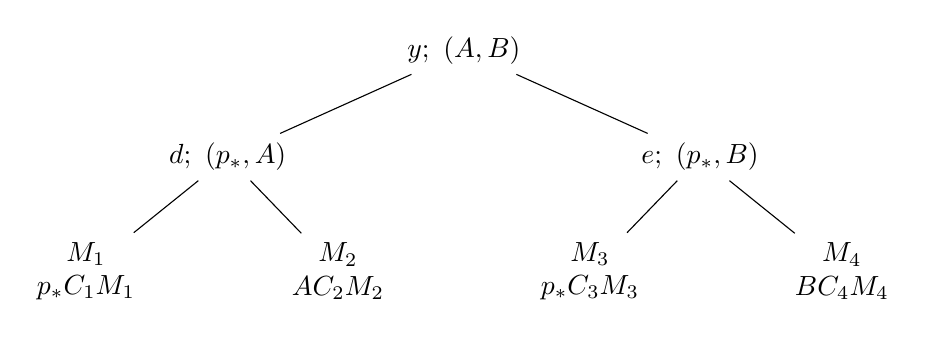
\begin{tikzpicture}
  \node (n) at (0,0) {$y;\ (A,B)$};
  \node (l) at (-3,-1.35) {$d;\ (p_*,A)$};
  \node (r) at (3,-1.35) {$e;\ (p_*,B)$};
  \node[align=center] (ll) at (-4.8,-2.8)
        {$M_1$\\$p_*C_1M_1$};
  \node[align=center] (lr) at (-1.6,-2.8)
        {$M_2$\\$AC_2M_2$};
  \node[align=center] (rl) at (1.6,-2.8)
        {$M_3$\\$p_*C_3M_3$};
  \node[align=center] (rr) at (4.8,-2.8)
        {$M_4$\\$BC_4M_4$};
  \draw (n)--(l) (n)--(r) (l)--(ll) (l)--(lr)
        (r)--(rl) (r)--(rr);
 \end{tikzpicture}
 \caption{A quartet with its ordered current entries.  Here $A,B$ are
 fixed local units, unrelated to the summand sets, and $d-e=y$.
 The shared entry $p_*$ is reconstructed and varies according to
 \eqref{eq:tree-p-square}.  Holding $M_2$
 or $M_4$ uses a residual entry $A$ or $B$; holding $M_1$ or $M_3$
 uses the reconstructed entry $p_*$.}
 \label{fig:tree-quartet}
\end{figure}

Orient the moving leaf as free in each pair.  Division of the formulas
in \eqref{eq:src36} gives
\begin{equation}\label{eq:tree-held-square}
 \frac{t_L}{d}=\text{a fixed unit}\times H_{\mathrm{held},L}^2,
 \qquad
 \frac{t_R}{e}=\text{a fixed unit}\times H_{\mathrm{held},R}^2.
\end{equation}
For example, if the free leaf is the first child of the left pair,
the constant in the first identity is
$D's_{\mathrm{free}}/(s_{\mathrm{held}}s_{\mathrm{pair}})$;
the opposite orientation gives the same form with the two bottom
frequencies interchanged.  At the quartet root, another direct
consequence of \eqref{eq:src36} is
\begin{equation}\label{eq:tree-p-square}
 p_*^2=\frac{s_+s_-}{s_nD'u_n^2}\frac{y}{de}.
\end{equation}
If the held entry in Figure~\ref{fig:tree-quartet} is the residual
$A$ or $B$, \eqref{eq:tree-held-square} therefore has the first of
the following forms; if it is $p_*$, use
\eqref{eq:tree-p-square} to obtain the second:
\begin{equation}\label{eq:tree-friendly-bad}
 t_L=\lambda_Ld\ \text{or}\ \lambda_L/e,
 \qquad
 t_R=\lambda_Re\ \text{or}\ \lambda_R/d.
\end{equation}
Call the first choice on either side friendly and the second bad.
The parameters $\lambda_L,\lambda_R$ are fixed unit multiples of the
squares of the two held leaf variables.  The multiples may depend on
the fixed parent data and on $y$, but not on the held variables.  Since
those variables are independent uniform units, the two parameters
are independent uniform square-coset variables.

For fixed held variables the parent ratio $d/e$ is a fixed unit times
the inverse square of the moving coordinate.  The local value depends
on this ratio, rather than on its square-root choice.  Indeed changing
the moving coordinate to its negative changes $p_*$ to its negative,
while \eqref{eq:tree-friendly-bad} only used its square; the arguments
within either pair are determined by their ratio and their difference.
Apply \eqref{eq:tree-square-pullback}, and then dominate the two
square-coset laws of the held parameters by full independent unit laws.
The latter domination is applied to a nonnegative squared coefficient
and costs at most four.  On changing from $d/e$ to $d-e=y$, the
normalization changes by the bounded factor $q/(q-1)$.  We obtain a
constant times
\begin{equation}\label{eq:src41}
 \sum_{\nu^2=\rho^{\pm1}}
 \E_{\lambda_L,\lambda_R\in U}
 \left|\frac1q\sum_{\substack{d,e\in U\\d-e=y}}
 h_L(d,t_L)h_R(e,t_R)\nu(d/e)\right|^2.
\end{equation}
The sign allows either Mellin convention.  All invalid ratios are
encoded by the zero definitions of the functions $h$; in particular,
the parent ratio $1$ has no valid $(d,e)$ with $d-e=y\ne0$.

To check the sum over $\rho$ in \eqref{eq:src39}, it suffices to sum
over all $\nu$.  For $y\ne0$, the map $t=d/e$ is a bijection from
$U\setminus\{1\}$ to the unit solutions of $d-e=y$, with
$d=yt/(t-1)$ and $e=y/(t-1)$.  Mellin Parseval, followed by the
independent $\lambda_L,\lambda_R$ averages, bounds this sum by a
constant times
\[
 \frac1{q-1}\sum_{\substack{d,e\in U\\d-e=y}}R_L(d)R_R(e).
\]
Its mean over $y\in U$ is bounded by \eqref{eq:tree-R-mean}.

For the small bound at a fixed $\nu$, extend the nonnegative $y$ average
to all of $\F_q$, paying at most $q/(q-1)$.  Expand both $h$ factors
in Mellin characters $\chi,\psi$.  Orthogonality in the independent
parameters separates their squared coefficients.  Additive convolution
Parseval then reduces the bound to
\begin{equation}\label{eq:tree-twisted-convolution}
 \sum_{a,\chi,\psi}
        |\widehat{P_\chi\alpha}(a)|^2
        |\widehat{P_\psi\beta}(-a)|^2.
\end{equation}
Each pair uses its own choice of $\sigma,g_*$ in its $P$.  The twists
are listed explicitly below; all are zero at zero:
\[
\begin{array}{c|cc}
 \text{choices}&\alpha&\beta\\ \hline
 \text{friendly, friendly}&\nu\chi&\overline\nu\psi\\
 \text{friendly, bad}&\nu\chi\overline\psi&\overline\nu\\
 \text{bad, friendly}&\nu&\overline\nu\psi\overline\chi\\
 \text{bad, bad}&\nu\overline\psi&\overline\nu\overline\chi
\end{array}
\]
For example, the left friendly term contributes $\chi(d)$ and the
left bad term contributes $\overline\chi(e)$, which explains all four
rows.  If the left choice is friendly, the second twist is independent
of $\chi$.  Apply \eqref{eq:src42} to the sum over $\chi$, uniformly
in the remaining index and $a$.  The remaining sum is bounded since
additive Parseval gives
\[
 \sum_{\psi,a}|\widehat{P_\psi\beta}(a)|^2
 \leq\sum_\psi\E_{d\in\F_q}|P_\psi(d)|^2\ll1;
\]
here $\beta$ may depend on $\psi$.  This bounds
\eqref{eq:tree-twisted-convolution} by
$O(\eps_q^4+q^{-1/2})$.  The right friendly case is symmetric.

\subsection{The case of two bad choices}

It remains to bound \eqref{eq:tree-twisted-convolution} when
$\alpha=\nu\overline\psi$ and
$\beta=\overline\nu\overline\chi$.  For a nonprincipal character
$\alpha$, the additive Fourier transform of $\alpha$ has constant
modulus $q^{-1/2}$ on nonzero frequencies, and equals zero at zero.
For clarity, the needed Gauss identity follows by substituting
$x\mapsto x/t$ in $\sum_x\alpha(x)e_q(tx)$ for $t\ne0$; its
modulus is $\sqrt q$, because
\[
 \left|\sum_x\alpha(x)e_q(x)\right|^2
 =\sum_{u\in U}\alpha(u)\sum_{z\in U}e_q((u-1)z)
 =(q-1)-\sum_{u\ne1}\alpha(u)=q.
\]
Consequently, with harmless unit factors and a possible reflection
of the frequency,
\begin{equation}\label{eq:tree-Gauss-convolution}
 |\widehat{P_\chi\alpha}(a)|
   =q^{-1/2}\left|\sum_b w_\chi(b)\overline\alpha(a-b)\right|.
\end{equation}

Let $w\geq0$ be any weights of mass $J$ and let $r_w=\sum_b w(b)^2$.
Multiplicative orthogonality yields
\begin{equation}\label{eq:tree-fourth-moment}
 \frac1{q-1}\sum_{\alpha\in\widehat U}\sum_a
       \left|\sum_b w(b)\alpha(a-b)\right|^4
 \leq 2q r_w^2+J^4.
\end{equation}
Indeed, after expansion, a nonzero term requires
\[
 (a-b_1)(a-b_2)=(a-b_3)(a-b_4)\ne0.
\]
When the two unordered pairs of $b$'s agree, their total weight is
at most $2r_w^2$ and there are at most $q$ values of $a$.  Otherwise,
subtracting the two monic quadratics gives a nonzero polynomial of
degree at most one, so there is at most one value of $a$.  The total
weight of all these latter quadruples is at most $J^4$.

The principal character alone contributes
\[
 \frac1{q-1}\sum_a(J-w(a))^4
 \geq\frac{qJ^4-4J^3\sum_aw(a)}{q-1}
 =J^4-\frac{3J^4}{q-1}.
\]
Subtract this contribution in \eqref{eq:tree-fourth-moment} before
applying \eqref{eq:tree-Gauss-convolution}.  Since the masses $J$ of
our $w_\chi$ are uniformly bounded, for each $\chi$ this gives
\[
 \sum_{\alpha\ne1,a}|\widehat{P_\chi\alpha}(a)|^4
 \leq2r_\chi^2+O(q^{-2}).
\]
Summing over $\chi$ and using \eqref{eq:src40}, we obtain
\begin{equation}\label{eq:tree-all-nonprincipal-fourth}
 \sum_{\chi,\alpha\ne1,a}|\widehat{P_\chi\alpha}(a)|^4
 \ll\eps_q^2+q^{-1}.
\end{equation}
When both twists in \eqref{eq:tree-twisted-convolution} are
nonprincipal, Cauchy--Schwarz bounds it by the geometric mean of two
sums of this form.  This is legitimate because at fixed $\nu$ the map
$(\chi,\psi)\mapsto(\chi,\nu\overline\psi)$ is bijective, and the
corresponding assertion holds for the other factor.

We also record the principal cases explicitly.  Because the principal
character is zero at zero, its additive transform is
\begin{equation}\label{eq:tree-principal-correction}
 \widehat{P_\chi\ind_U}(a)=w_\chi(a)-\frac{P_\chi(0)}q.
\end{equation}
Thus its Fourier maximum is $O(\eps_q^2+q^{-1})$, and its squared
Fourier norm is no greater than $r_\chi$ by Parseval on the original
functions.  If $\alpha$ is principal, then $\psi=\nu$ is fixed.
When $\beta$ is nonprincipal,
\eqref{eq:tree-Gauss-convolution} and the bounded mass of
$w_\psi$ bound the other Fourier factor by $O(q^{-1/2})$ uniformly.
Summing the first squared factor over $\chi,a$ costs $O(1)$ by
\eqref{eq:tree-total-r}; this part is $O(q^{-1})$.
The case with the two roles exchanged is identical.  If both twists
are principal, both indices are fixed.  Apply the small Fourier
maximum in \eqref{eq:tree-principal-correction} to one factor and
the bounded squared norm to the other.  This contributes
$O(\eps_q^4+q^{-2})$.

The two-bad case of \eqref{eq:tree-twisted-convolution} is therefore
$O(\eps_q^2+q^{-1})$.  Together with the friendly estimates this
proves the first assertion of \eqref{eq:src39} for
\eqref{eq:src41}.  Adding the finitely many orientation choices and
the same-pair majorants completes the construction of $B_\rho$ and
$B_0$.

\subsection{Completion of the cycle estimate}

Return to the projection in \eqref{eq:tree-projection-reduction},
conditioning again on the products in all bottom quartets.
Orthogonality in
the independent moving coordinates gives a sum of products of
$|a_{j,\rho_j}|^2$, with squared untouched-quartet values as the other
factors.  Average the held variables.  The bounds already proved
dominate this expression by
\[
 \sum_{\prod_j\rho_j^{\delta_j}=1}
             \prod_{j=1}^t B_{\rho_j}(y_j)
             \prod_{j\notin\mathrm{cycle}}B_0(y_j).
\]
The actual joint distribution of quartet arguments on valid ancestor
points is dominated by a constant depending only on $l$ times
independent uniform unit measure, by the horizontal-level density
bound proved above.  Since this last display is nonnegative, we may
use that domination without any pointwise control of $g$.

Put $b_\rho=\E_{y\in U}B_\rho(y)$ and
$b_0=\E_{y\in U}B_0(y)$.  One character in
\eqref{eq:tree-cycle-relation} is determined uniquely by the others.
Consequently
\[
 \|\mathcal PW_1\|_2^2
 \leq C_l\bigl(\sup_\rho b_\rho\bigr)
                 \left(\sum_\rho b_\rho\right)^{t-1}
                 b_0^{r/4-t}
 \ll_l\eps_q^2+q^{-1/2}.
\]
If the cycle consists of two parallel edges, $t=1$ and its sole
character is principal; the same inequality simply uses
$b_1\leq\sup_\rho b_\rho$.  Thus this degenerate cycle requires no
separate structural assumption.  Equation
\eqref{eq:tree-projection-reduction} proves the quantitative statement
of Lemma~\ref{lem:tree-comparison}, and hence \eqref{eq:src38}.

For the later application, the exact transforms $g_p$ in
\eqref{eq:src27} satisfy $g_p(0)=0$ and $\E|g_p|^2=1$ by centering
and additive Parseval.  On the chosen spectator subset their mixed
correlation parameters tend to zero uniformly.  Once independent
unit bulk residues have been obtained in Section~\ref{sec:arithmetic},
Lemma~\ref{lem:tree-comparison} may therefore be applied separately
at every spectator prime.  The zero convention in the diagram retains
the requirement that every reconstructed entry be a unit at that
prime.

\section{A positive statistic and its binary-tree transfers}
\label{sec:construction}

We combine the size and collision estimates with the Fourier supply
of Proposition~\ref{prop:supply} to construct a nonnegative statistic.
Poisson summation will turn it into an amplitude.  The transfers
propagate a quantitative lower bound once their diagonals are controlled;
Section~\ref{sec:conclusion} will bound the same amplitude from above
by averaging over arrangements of its prime variables.

The pivot extraction, extension to positive integers, and doubling of
the remaining template follow the architecture of
Section~\ref{sec:characters}.  The exact residue-mask transforms carry
no prescribed multiplicative-character phase, so the anchor cancellation
is replaced by a common outside list of spectator primes, where
Lemma~\ref{lem:tree-comparison} compares the paired histories.

All parameters introduced in this section are new; in particular, the
letters $L,k,m$ no longer denote parameters from the preceding character
arguments.

\subsection{Scales and prime priors}

Let $L\to\infty$.  The transfer depth $k$ will be a sufficiently large
fixed positive integer, chosen before $L$ tends to infinity.  Put
\[
 h=e^{.01L},\qquad z=k^4,\qquad
 m=2\lfloor zL/2\rfloor,\qquad r_j=2^{j-1}\quad(1\le j\le k).
\]
The notation $o_k(m)$ and $O_k(1)$ permits dependence on all parameters
that are fixed before $L$.  In bounds of the form $Cm$ or $C2^lm$,
however, $C$ will be independent of $k$ and of the large gap constants
introduced below, once $k$ and then $L$ are sufficiently large.  The
threshold on $L$ may depend on these fixed choices.

Choose fixed positive constants $B_s,B_D,B_z$, with their order of
choice specified in Section~\ref{sec:conclusion}, and define
\begin{align}
 \Delta_0&=(B_s+8\log z)m,\notag\\
 \Delta_j&=r_j(B_D+B_z\log z+.4\log r_j)m
       \qquad(1\le j\le k),\notag\\
 E_l&=\Delta_0+\sum_{j=1}^l\Delta_j+2^l\sqrt m,\notag\\
 V_l&=e^{E_l}\qquad(0\le l\le k).
 \label{eq:src43}
\end{align}
Thus $\log V_l=O_k(m)$.  In particular, all frequencies used below
are smaller than every sampled prime, since even the smallest prime
range has lower endpoint $\exp(\exp(.0005L))$.

Fix a nonnegative smooth function $\varphi$ supported on $[-1,1]$
such that
\[
 \sum_{n\in\Z}\varphi(t-n)=1\qquad(t\in\R).
\]
Then $0\le\varphi\le1$ and $\int_{\R}\varphi(t)\,dt=1$.
For a center $c$, the \emph{log-cell prior} is the probability measure
on primes proportional to
\[
                 \frac{\varphi(\log p-c)}p.
\]
Except for the giant-prime prior defined shortly, all prime priors
will omit a set $\mathcal E_L$ of at most two prime values.  This set
is fixed for each $L$; Section~\ref{sec:arithmetic} specifies its
choice from the two possible Page exceptional conductors.  Every
abundance assertion in this section holds uniformly after any such
deletion.  A nongiant cell is therefore normalized by
\[
 Z_c=\sum_{\substack{p\ \text{prime}\\p\notin\mathcal E_L}}
                 \frac{\varphi(\log p-c)}p.
\]
For all the cell centers used here, the prime number theorem and
partial summation give $Z_c\sim c^{-1}$.  The same statement holds
without the deletion.  They also give
\[
 \sum_p\frac{\log p}{p}\varphi(\log p-c)=1+o(1).
\]
The errors are uniform as the centers in our specified ranges tend
to infinity.  Deleting two prime values does not change these
asymptotics.

By \eqref{eq:src28}, there is a block $[G_0,G_0+h]$ in log-prime
coordinates, contained in the range of that estimate, such that the
primes satisfying its two conditions have total $(\log p)/p$ weight
at least $c_0h$, for a fixed $c_0>0$.  Here and below a prime satisfying
those conditions is called favorable.  To see the block assertion,
partition
$[e^{.05L},e^{.9L}]$ into intervals of length $h$, apart from the two
end pieces.  On each full block the log coordinate varies by a
relative $o(1)$, uniformly in the block.  If every block had favorable
$(\log p)/p$ weight at most $ch$, summing these bounds after division
by the left log coordinate would give favorable harmonic weight at
most $(.85c+o(1))L$.  A sufficiently small fixed $c$ contradicts
\eqref{eq:src28}.  Mertens' estimates make the two end pieces
negligible in this calculation.

Set
\[
                   \log X=2G_0+2^{k+1}h,
       \qquad A'=A\cap[X^{9/10},X].
\]
The whole chosen block lies below the prime cutoff in
\eqref{eq:src2} for the uniform measure on $A'$.  Indeed,
$\log\sqrt X=G_0+2^kh$, whereas the block ends at $G_0+h$, and the
loss from the logarithmic denominator in that cutoff is only
$O(\log\log X)=O(L)$.

Use the transforms $F_p,g_p$ from \eqref{eq:src27}, with the
normalization
\[
 g_p(b)=\sqrt p\,\E_{x\bmod p}F_p(x)e_p(-bx),\qquad
 F_p(x)=p^{-1/2}\sum_{b\bmod p}g_p(b)e_p(bx).
\]
For a favorable prime put
\[
 \widetilde g_p(b)=
 \begin{cases}
   g_p(b)/|g_p(b)|,&g_p(b)\ne0,\\
   0,&g_p(b)=0,
 \end{cases}
\]
and put $\widetilde g_p=0$ at every other prime.  Let
$\widetilde F_p$ be its inverse transform with the same
normalization.  Conjugate symmetry of $g_p$ implies that
$\widetilde F_p$ is real.  Also
\[
 \E_x\widetilde F_p(x)=0,
 \qquad \E_x|\widetilde F_p(x)|^2
      =\E_b|\widetilde g_p(b)|^2\le1.
\]
For a favorable prime, Parseval and the definition of $F_p$ give
\[
 \E_{x\in S_p}\widetilde F_p(x)
   =\sqrt{\frac{1-\sigma_p}{\sigma_p}}\,
        \E_b|g_p(b)|\ge\frac{\delta_0}{\sqrt2}.
\]

There is an integer center $G$, whose log-cell support is contained
in $[G_0,G_0+h]$, for which
\begin{equation}
 \E_{\substack{p\ \text{in the cell at}\ G\\a\in A'}}
                     \widetilde F_p(a)\ge c_1>0.
 \label{eq:src44}
\end{equation}
The giant prior in this display includes all primes in its cell.
Here is why the collision estimate applies to these possibly
unbounded inverse transforms.  If $\mu_p$ is the projection of the
uniform probability on $A'$, then Cauchy--Schwarz gives
\[
 \left|\sum_{x\bmod p}
    (\mu_p(x)-U_{S_p}(x))\widetilde F_p(x)\right|^2
       \le p\,\|\mu_p-U_{S_p}\|_2^2.
\]
Consequently \eqref{eq:src2} bounds the sum of these squared errors
with weight $(\log p)/p$ by $O(L)$.  The total such weight on the
block is $O(h)$, so its weighted sum of absolute errors is
$O(\sqrt{Lh})=o(h)$.  The favorable uniform means, on the other
hand, have a positive sum of order $h$.  Partitioning by the integer
translates of $\varphi$, and deleting the bounded-width end strips,
therefore supplies a cell with a positive average empirical mean.
Replacing $(\log p)/p$ by $1/p$ in this cell does not change this
conclusion: the log coordinate has relative variation $o(1)$, and
the same error bound applies.  This proves \eqref{eq:src44}.

Fix this $G$.  Write
\begin{equation}
 Z_G=\sum_{p\ \text{prime}}\frac{\varphi(\log p-G)}p,
 \qquad
 \mu_G(p)=\frac{\varphi(\log p-G)}{pZ_G},
 \qquad c_g=\log Z_G^{-1}.
 \label{eq:construction-giant-prior}
\end{equation}
We have $Z_G\sim G^{-1}$, and hence
$c_g=\log G+O(1)\le .91L$ for sufficiently large $L$.
The coefficient in this last bound is independent of the gap
constants and of $k$.

\subsection{The initial lists and positive statistic}

A \emph{half-list} consists of the following independent positions:
\begin{enumerate}[label=(\roman*)]
 \item one giant with prior $\mu_G$, using the test
       $\widetilde F_p$;
 \item $m/2$ bulk positions, with their common prior proportional to
       $1/p$ on
       $.004L\le\log\log p\le .006L$,
       omitting $\mathcal E_L$;
 \item $m/2$ spectator positions, with their common prior proportional
       to $1/p$ on a subset of
       $.0005L\le\log\log p\le .001L$
       of harmonic mass $\gg L$, omitting $\mathcal E_L$, on which
       \eqref{eq:src27} holds uniformly with a bound tending to zero;
 \item three top positions and two compensation positions of each
       type $j=1,\ldots,k$, with cell priors chosen below.
\end{enumerate}
Every nongiant position uses the exact test $F_p$.  The spectator
subset exists by Corollary~\ref{cor:mixed-flatness}; its exceptional
threshold can be chosen slowly enough that all the stated
conclusions hold uniformly on the retained subset.  The bulk and
spectator harmonic normalizing masses are both between fixed
positive multiples of $L$.

Let $S_b,S_d$ be the sums of the log primes at the bulk and spectator
positions of one half-list.  Include in its weight the two factors
\[
                   \varphi(S_b-t_b)\varphi(S_d-t_d).
\]
These are weights, not conditioning of any prior.  Choose integer
centers $t_b,t_d$ so that, for each of the two groups, the expectation
of its cutoff together with the restriction
$1/3\le\sigma_p\le2/3$ at all its positions is at least $e^{-Cm}$.
Such choices follow directly from the partition of unity.  Almost
all the probability of a single position is balanced, by
\eqref{eq:src27} or \eqref{eq:src2}; for sufficiently large $L$ the
probability that all positions in that group are balanced is at
least $2^{-m/2}$.  Each possible log sum lies in an interval admitting
at most $\exp(O(L)+O(\log m))$ relevant integer centers.  At least
one center thus has the required weighted mass.  In particular,
\[
                    t_b,t_d=o_k(h).
\]

Call the bulk and top positions \emph{protected}.  For the full list
of two half-lists, define the target log sum $J$ for the protected
positions and the target log sum $w_j$ for compensation type $j$ by
\begin{equation}
 J=\frac{\log X-2G-2t_d+\Delta_0+\sum_{j=1}^k\Delta_j}{2^k},
 \qquad
 w_j=J+\sum_{i>j}w_i-\frac{\Delta_j}{r_j}.
 \label{eq:src45}
\end{equation}
The second definition is made successively for $j=k,k-1,\ldots,1$.
It gives
\[
 J\asymp h,\qquad
 w_j=(2^{k-j}+o_k(1))J,
 \qquad
 J+\sum_{j=1}^kw_j=2^kJ-\sum_{j=1}^k\Delta_j.
\]
Choose the three top cell centers in a fixed small relative neighborhood of
$(J-2t_b)/6$, with their sum equal to $(J-2t_b)/2+O(1)$.
For the two positions of type $j$, choose centers in a corresponding
neighborhood of $w_j/4$, with sum $w_j/2+O(1)$.  Neighborhoods of
relative radius $.03$ suffice to keep different compensation types,
top positions, bulk positions, spectator positions, and giants in
pairwise disjoint prime ranges.

All these top and compensation centers can be chosen so that the
balanced primes have a fixed positive fraction of the cell prior.
Indeed, these primes also lie below the cutoff in
\eqref{eq:src2}.  A cell in which a fixed positive fraction is
unbalanced contributes a fixed positive amount to the nonnegative
imbalance term in that estimate.  Since the translates of
$\varphi$ sum to one, only $O(L)$ integer centers can fail the desired
balanced-fraction condition.  Each neighborhood available here has
length comparable to $h$, which is much larger than $L$.
For a prescribed rounded pair sum, exclude a bad center and its
reflection about that sum; this excludes only $O(L)$ choices.
For a triple, choose the first two centers in slightly smaller
neighborhoods.  Among the resulting pairs only an $O(L/h)$ fraction
have a bad third center determined by the rounded sum.  This gives
the required centers while respecting all ranges.  On the bulk
cutoff, the protected log sum of each half-list is now
$J/2+O(1)$.

Let $T(n)$ be the expectation over one half-list of the product of
all its tests at $n$, multiplied by the two log-sum cutoffs.  For
$a\in A'$, every exact local test is
\[
                     F_p(a)=\sqrt{\frac{1-\sigma_p}{\sigma_p}}>0.
\]
This value is independent of the choice of $a\in A'$: all these
primes are sufficiently small for the defining residue restriction
on $A$ to apply.  The expectation of the product of exact tests and
the cutoffs is therefore a positive scalar $c_L$, independent of
$a$, with $c_L\ge e^{-Cm}$.  This lower bound follows by restricting
every nongiant position to balanced primes; each local value is at
least $2^{-1/2}$, and the preceding bin and cell choices give the
required mass.  Thus
\[
                    T(a)=c_L\E_{p\sim\mu_G}\widetilde F_p(a).
\]
Take the nonnegative Schwartz function $\psi$ used in the quadratic
argument, with compactly supported smooth Fourier transform and a
positive lower bound on $[0,1]$.  The tests are real, so $T(n)^2$ is
nonnegative.  Equation~\eqref{eq:src44}, Jensen's inequality on $A'$,
and the lower bound in \eqref{eq:src1} give
\begin{equation}
              I:=\sum_{n\in\Z}\psi(n/X)T(n)^2
                   \ge \sqrt X\,e^{-Cm}.
 \label{eq:src46}
\end{equation}
The logarithmic loss in $|A'|$ is absorbed here because
$\log\log X=O(L)$ and $m\asymp k^4L$.  Notice that this argument
uses the mean of the giant test and its square; it does not require
the giant test to be pointwise nonnegative.

\subsection{Removing repeated primes and applying Poisson summation}

Expand $T(n)^2$ using two independent half-lists.  Let $M$ be the
product of all positions, counted with multiplicity.  On the cutoff
support,
\[
 \log M=2G+2t_d+J+\sum_{j=1}^kw_j+O_k(1)
        =\log X+\Delta_0+O_k(1).
\]
We may discard the tuples with repeated prime values, with a
negligible error relative to \eqref{eq:src46}.  We give the estimate
because no cancellation estimate for repeated local factors is
being assumed.

For a tuple containing a repetition, the product of its distinct
primes, denoted $Q$, satisfies
\[
 Q\ll_k X e^{\Delta_0}/\exp(\exp(.0005L))=o(X).
\]
The product of the local tests is periodic modulo $Q$.  Compact
Fourier support of $\widehat\psi$ implies that its smoothed sum is
exactly $X\widehat\psi(0)$ times its residue mean, for sufficiently
large $L$.  If any prime occurs once, that residue mean is zero by
the mean-zero property of its test and CRT.  If a prime occurs with
multiplicity $e\ge2$, its contribution to the absolute residue
mean is at most $p^{e/2-1}$.  Indeed every local test has probability
$L^2$ norm at most one, hence supremum at most $\sqrt p$; apply
Cauchy--Schwarz to two factors and use the supremum bound for the
others.  This argument also covers factors assigned different
roles at the same prime.

The probability of any prescribed ordered tuple is at most
\[
            M^{-1}L^{-2m}\exp(Cm+O_k(1)).
\]
There are $2m$ broad-band positions.  Each contributes a
normalization of size at most $C/L$.  The remaining $4k+8$ cell
positions have combined normalization at most $\exp(O(kL)+O_k(1))$,
which is $\exp(Cm+O_k(1))$ with $C$ independent of large $k$ because
$m\asymp k^4L$.  Since
$\prod_{p\mid Q}p^{e_p/2-1}=M^{1/2}/Q$, the absolute contribution
of tuples in which every prime occurs at least twice is at most
\[
 \sqrt X\exp(-\Delta_0/2+Cm+O_k(1))L^{-2m}
               \sum_{\rm tuples}\frac1{\prod_{p\ \text{distinct}}p}.
\]
Put $b=2m+4k+8$.  The harmonic mass of the union of all prime ranges
is $O(L)$.  Assigning the $b$ labeled positions to $i$ distinct
values, and then dropping restrictions for an upper bound, gives
\[
 \sum_{\rm tuples}\frac1{\prod_{p\ \text{distinct}}p}
    \le \sum_{i=1}^{b}\frac{i^b(CL)^i}{i!}
    \le b^b e^{CL}.
\]
Thus the repeated-prime contribution is bounded by
\[
 \sqrt X\exp\left(-\frac{\Delta_0}{2}
                +(2\log z+C)m+o_k(m)\right).
\]
Choosing $B_s$ sufficiently large makes this negligible in
\eqref{eq:src46}.  The constant required here is independent of the
later gap constants and of sufficiently large $k$.

Retain only tuples with all positions distinct, and let $\eta_0$ be
their Poisson expression divided by $\sqrt X$.  We have shown that
\begin{equation}
                        |\eta_0|\ge e^{-B_*m}
 \label{eq:src47}
\end{equation}
for a fixed $B_*$ independent of $B_D,B_z$ and $k$.  The same
$B_*$ may be used for all sufficiently large admissible $B_s$.

\subsection{Templates, coefficients, and support conventions}
\label{subsec:coefficient-support}

Keep the $m$ spectator positions of the two half-lists, with their
original half-list roles, as one outside list $\mathbf d$, and write
$d$ for their product.  This list will never be duplicated.  All
other positions form the ordered regular template $\mathcal I_0$;
its two giants are labeled $+$ and $-$ in a fixed order.

At step $j$, split $\mathcal I_{j-1}$ into the pivot positions and
the remaining template $H$.  The pivot product is $P=pu$, where
$p$ is the $+$ giant and $\mathbf u$ is the ordered list of all
current compensation positions of type $j$, with product $u$.
Unlike the whole-pivot extension in Section~\ref{sec:characters},
here only the giant $p$ will be extended to positive integers.
The entries of $\mathbf u$ retain their actual-prime priors.
Thus $H$ contains the other giant, all protected positions, and all
positions of types $i>j$.  Form
$\mathcal I_j=(H_+,H_-)$ from two copies of $H$, labeling their
giants $+$ and $-$, respectively.  Whenever a template or a part of
one is sampled, its positions have independent copies of their
specified priors.

Before step $j$, there are $r_j$ copies of the full protected list
of two half-lists, and $r_j$ copies of each compensation type not
yet removed.  In particular $\mathbf u$ has $4r_j$ positions.
On the inherited protected bins,
\begin{align}
 \log u&=r_jw_j+O_k(1),\notag\\
 \log H&=T_H+O_k(1),\qquad
 T_H=G+r_j\left(J+\sum_{i>j}w_i\right)
       =G+r_jw_j+\Delta_j.
 \label{eq:src48}
\end{align}
Here a template and its product are denoted by the same letter only
when no confusion can result.

If $R$ is the product of distinct actual regular prime values, put
\[
 G_R(b)=\prod_{\ell\mid R}
             g_\ell^{\rm reg}\bigl(b/(R/\ell)\bmod\ell\bigr),
\]
where $g_\ell^{\rm reg}=\widetilde g_\ell$ on a giant position and
$g_\ell^{\rm reg}=g_\ell$ on every small regular position.  Field
fractions always have unit denominators.  This expression is used
only on the pairwise coprime support, and is extended by zero when
that support fails.  The amplitudes will have the form
\begin{equation}
 \eta_l=\E_{\mathbf d,\mathcal I_l}
       \sum_{0<|s|\le V_l}G_R(s/d)A_l(s),
                  \qquad R=\prod\mathcal I_l.
 \label{eq:src49}
\end{equation}
The factor $G_R(s/d)$ depends on the actual regular prime values and
their product, so it is unchanged when the bulk values are reassigned
among their positions.  The coefficient $A_l$ will contain the
spectator factors and all arrangement-dependent history weights and
support conditions.  This separates the common factor from the
coefficient to be averaged over arrangements.
The outer positions in this expectation are actual primes.
The coefficient $A_l$, unlike $G_R$, will also be defined when its
two giant entries are positive integers.

We specify all its support conventions.  A history is a full binary
tree of depth $l$, with leaves at level zero.  Each node at level
$i$ has a nonzero signed integer frequency of magnitude at most
$V_i$.  At every state in a history require pairwise coprimality of
all its current slots and the outside list $\mathbf d$.  Its two
current giant values must also be units against \emph{every}
frequency at that node or below it.  These last restrictions may
always be added at an actual top, without changing an expression:
actual giant primes exceed every frequency in any of the finitely
many possible history levels.  Once added, they are kept when a
giant is extended to an integer.  These requirements are imposed
termwise on complete histories; they include cross-branch
frequency tests for either current giant.  A newly inserted pivot
is a current giant in its child states, so it is subject to their
subtree tests.  Failed support conditions give zero.

At level zero set
\begin{equation}
 \begin{split}
 A_0(s)={}&\left(\frac{X}{dR}\right)^{1/2}
             \widehat\psi\left(-\frac{sX}{dR}\right)\,
       \prod_{\rm halves}\varphi(S_b-t_b)\varphi(S_d-t_d)\\
 &\hspace{13mm}\cdot
       \prod_{q\mid d}
          g_q\bigl(s/((d/q)R)\bmod q\bigr),
 \end{split}
 \label{eq:src50}
\end{equation}
on this support, and zero otherwise.  The half-list spectator
weights use the original outside roles of $\mathbf d$.
Formula~\eqref{eq:src49} with $l=0$ is the distinct-tuple Poisson
formula.  Indeed the local inverse expansions contribute
$(dR)^{-1/2}$, and Poisson summation followed by division by
$\sqrt X$ gives the factor $\sqrt{X/(dR)}$ in
\eqref{eq:src50}.  The zero frequency vanishes since the local
transforms vanish at zero.  On the cutoffs,
$dR/X=\exp(\Delta_0+O_k(1))$; the additional $\sqrt m$ in
$E_0$ therefore accommodates the fixed compact support of
$\widehat\psi$.

For the recursive definition of $A_j$, a current state is
$\mathcal I_j=(H_+,H_-)$ with root frequency $s$.
Sum over $v,w$ with $0<|v|,|w|\le V_{j-1}$, and independently sample
the type-$j$ vector $\mathbf u$ by its priors.  Restore the pivot by
\begin{equation}
                       p=\frac{vH_- - wH_+}{su}.
 \label{eq:src51}
\end{equation}
Retain it only if it is a positive integer.  The two child states
are copies of $\mathcal I_{j-1}$ with entries $(p,\mathbf u,H_+)$
and $(p,\mathbf u,H_-)$ in their prescribed roles.  Their giant
pairs, in order, are the inserted $p$ and the giant of $H_+$ or
$H_-$, respectively.  Keep the same outside list $\mathbf d$.
Multiply the two child coefficients, conjugating the right one,
by
\begin{equation}
                         u\varphi(\log p-G).
 \label{eq:src52}
\end{equation}
Sum and average these terms, imposing all the history restrictions
above.  In a formula, with state arguments displayed only here,
\begin{align*}
 A_j(s;\mathbf d,H_+,H_-)
   =\sum_{\substack{0<|v|\le V_{j-1}\\0<|w|\le V_{j-1}}}
       \E_{\mathbf u}\bigl[{}
       &u\varphi(\log p-G)
          A_{j-1}(v;\mathbf d,p,\mathbf u,H_+)\\
       &\cdot\overline{A_{j-1}(w;\mathbf d,p,\mathbf u,H_-)}
                              \bigr].
\end{align*}
The bracket is interpreted termwise after expanding the two child
histories, and is zero unless \eqref{eq:src51} and all their support
conditions hold.  Internal samples in the two children are
independent; only $\mathbf u$ at the present node is shared.
This defines $A_l$ for actual or integer giant entries, and includes
no transform attached to an integer giant.

Figure~\ref{fig:transfer-recursion} records the dependencies in this recursion.

\begin{figure}[tbp]
  \centering
  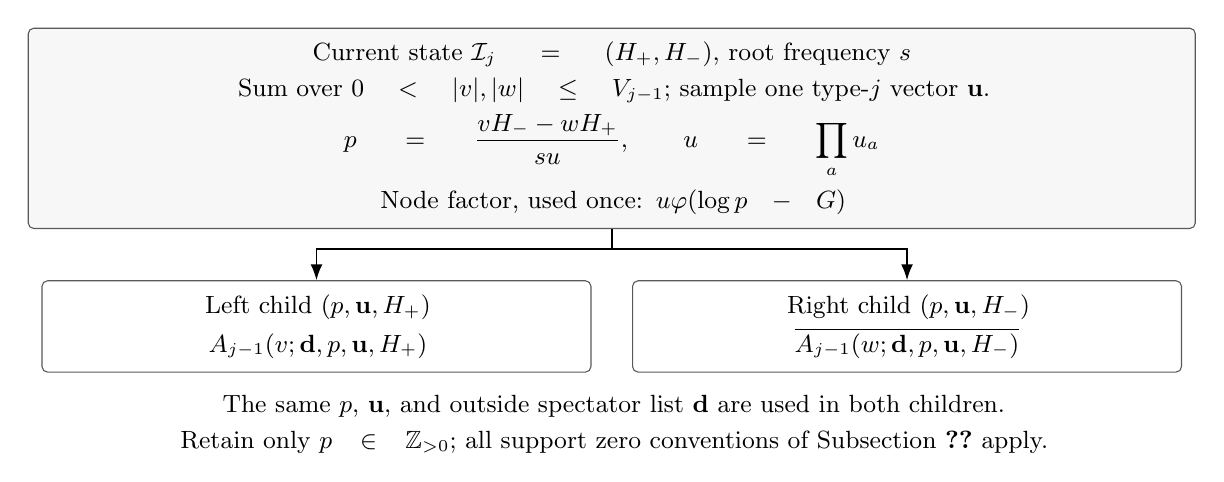
\begin{tikzpicture}[
    every node/.style={font=\small,align=center},
    transfer box/.style={
      draw=black!65,rounded corners=2pt,
      inner xsep=6pt,inner ysep=5pt
    },
    transfer arrow/.style={-{Latex[length=2mm]},line width=.6pt}
  ]
    \node[transfer box,fill=black!3,text width=14.4cm] (current) {
      Current state $\mathcal I_j=(H_+,H_-)$, root frequency $s$\\[2pt]
      Sum over $0<|v|,|w|\le V_{j-1}$;
      sample one type-$j$ vector $\mathbf u$.\\[3pt]
      $\displaystyle p=\frac{vH_- - wH_+}{su},
        \qquad u=\prod_a u_a$\\[3pt]
      Node factor, used once: $u\varphi(\log p-G)$
    };

    \node[transfer box,text width=6.55cm,anchor=north]
      (left) at ($(current.south)+(-3.75cm,-.65cm)$) {
      Left child $(p,\mathbf u,H_+)$\\[3pt]
      $A_{j-1}(v;\mathbf d,p,\mathbf u,H_+)$
    };
    \node[transfer box,text width=6.55cm,anchor=north]
      (right) at ($(current.south)+(3.75cm,-.65cm)$) {
      Right child $(p,\mathbf u,H_-)$\\[3pt]
      $\overline{A_{j-1}(w;\mathbf d,p,\mathbf u,H_-)}$
    };

    \coordinate (split) at ($(current.south)+(0,-.25cm)$);
    \draw[line width=.6pt] (current.south) -- (split);
    \draw[transfer arrow] (split) -| (left.north);
    \draw[transfer arrow] (split) -| (right.north);

    \node[anchor=north,text width=14.8cm,inner sep=0pt]
      at ($(left.south)!.5!(right.south)+(0,-.28cm)$) {
      The same $p$, $\mathbf u$, and outside spectator list $\mathbf d$
      are used in both children.\\[2pt]
      Retain only $p\in\mathbb Z_{>0}$;
      all support zero conventions of Subsection~\ref{subsec:coefficient-support} apply.
    };
  \end{tikzpicture}
  \caption{The coefficient recursion for $A_j(s)$:
    multiply the node factor by the two displayed child factors,
    with no prime-specific transform attached to the integer pivot $p$.
    Subsequent internal samples in the two descendants are independent
    in their underlying priors, before the complete-history support
    indicators are applied.}
  \label{fig:transfer-recursion}
\end{figure}

\subsection{The exact transfer and its diagonal}

We verify the relation between the successive expressions
\eqref{eq:src49}.  Fix $\mathbf d,p,\mathbf u$ at step $j$, put
$P=pu$, and group old terms according to
$t=v/H\pmod P$.  On the original prime support,
\[
 G_{PH}(v/d)=G_P(t/d)G_H(v/(Pd)).
\]
Let
\[
 B_t=\E_H
       \sum_{\substack{0<|v|\le V_{j-1}\\v/H\equiv t\ ({\rm mod}\ P)}}
                G_H(v/(Pd))A_{j-1}(v),
\]
with all inherited support conditions; invalid terms are zero.
The extracted row has counting squared norm at most $P$:
\[
                   \sum_{t\bmod P}|G_P(t/d)|^2\le P.
\]
This is CRT and the exact probability squared norm one at each
compensation prime, together with squared norm at most one at the
giant.  Cauchy--Schwarz in this row, followed by Jensen over the
outer probability measures, yields
\[
                  |\eta_{j-1}|^2
                    \le\E_{\mathbf d,p,\mathbf u}
                                  P\sum_{t\bmod P}|B_t|^2.
\]
Crucially, $B_t$ contains no prime-specific transform of the pivot
giant $p$.  It is defined for a positive integer $p$ by exactly the
same formulas, with the same coprimality and frequency filters.
Equation~\eqref{eq:construction-giant-prior} gives
$p\mu_G(p)=e^{c_g}\varphi(\log p-G)$ at primes.  Extending the
nonnegative sum to all positive integers gives
\begin{equation}
 |\eta_{j-1}|^2
   \le e^{c_g}\E_{\mathbf d,\mathbf u}
          \sum_{p\in\N}u\varphi(\log p-G)
                         \sum_{t\bmod pu}|B_t|^2.
 \label{eq:src53}
\end{equation}
Here the sum over $p\in\N$ means positive integers.

Expand the square using independent $H_+,H_-$ and child frequencies
$v,w$.  Separate the terms $vH_-=wH_+$ as the diagonal.
For every other term, the congruence of the two group indices
defines the nonzero signed integer
$s=(vH_--wH_+)/(pu)$, so the substitution is exactly
\eqref{eq:src51}.  It is one-to-one, with $p$ still any positive
integer in its cell.  Equations~\eqref{eq:src43} and
\eqref{eq:src48} show
\[
 \log|s|\le E_{j-1}+\Delta_j+O_k(1)<E_j.
\]
The margin is $2^{j-1}\sqrt m$, which tends to infinity.
All protected bins used in this size estimate are present in each
nonzero child history.

The actual lists $H_+,H_-$ cannot share a prime on such a term.
If $\ell$ divided both products, it would divide $s$, since it is
coprime to $pu$; but $\ell>|s|$.  At a prime of $H_+$ and a prime
of $H_-$, respectively, \eqref{eq:src51} gives
\[
                 v/P=s/H_-,\qquad -w/P=s/H_+.
\]
The inverse tests are real, so
$g_\ell^{\rm reg}(-b)=\overline{g_\ell^{\rm reg}(b)}$.
The two regular transforms therefore combine exactly into
$G_{H_+H_-}(s/d)$.  The remaining weights, histories, and inserted
pivot are precisely the recursive definition of $A_j$.
Additional giant-frequency tests at the new top are free because
its two giants are actual primes.  Consequently the off-diagonal
part of the extended expression in \eqref{eq:src53}, before
$e^{c_g}$, is exactly $\eta_j$.

Write $\mathcal D_j$ for its exact diagonal.  It is nonnegative, as
we now verify, and we have
\begin{equation}
                e^{-c_g}|\eta_{j-1}|^2
                         \le\mathcal D_j+\eta_j.
 \label{eq:construction-transfer-split}
\end{equation}
In particular the off-diagonal expression $\eta_j$ is real: the
extended square and its diagonal are real.

On the diagonal, all prime factors of $H_+$ and $H_-$ exceed the
frequencies, so $vH_-=wH_+$ forces $H_+=H_-$ as products and
$v=w$.  Grouping by this common product and frequency \emph{before}
expanding the square gives a common factor
$|G_H(v/(pud))|^2$ times the squared absolute value of the
prior-weighted sum of coefficients over its ordered arrangements.
This proves nonnegativity.  The common factor is independent of the
ordering: each prime uses the same local transform in every
arrangement, and the single giant in $H$ is fixed by its disjoint
range.  We may therefore drop its bounded giant factor in this
nonnegative expression.  The remaining multiplier is
\begin{equation}
 \mathcal G=\prod_{\ell\mid H_{\rm sm}}
       \left|g_\ell\bigl(v/(pud(H/\ell))\bmod\ell\bigr)\right|^2,
 \label{eq:src54}
\end{equation}
where $H_{\rm sm}$ consists of the small slots of $H$.

Now expand by bijections matching the slots in the two $H$ lists.
This counts every ordered counterpart once, since the prime values
within a valid $H$ are distinct.  Only matches within the same
prime band can occur.  In particular the giant matches itself and
bulk positions match bulk positions.

Fix a first ordered $H$.  For any prescribed counterpart ordering,
its point probability is $C_H/H$ times its smooth cell factors and
its role-membership indicators.  The normalizing constants satisfy
\begin{equation}
                 C_H\le L^{-r_jm}\exp(Cr_jm+O_k(1)).
 \label{eq:construction-counterpart-mass}
\end{equation}
Indeed there are $r_jm$ bulk positions, and $O(kr_j)$ cell positions.
The latter normalizations cost $\exp(O(kr_jL)+O_k(1))$, absorbed
uniformly by $\exp(Cr_jm)$ because $m\asymp k^4L$.
On simultaneous coefficient support, \eqref{eq:src48} allows us to
extract $C_He^{-T_H}$, leaving $e^{T_H}/H=O_k(1)$.
Normalize the external integer measure as
\begin{equation}
       \int f(p)\,d\mu_{\mathrm{ext}}(p)
          :=e^{-G}\sum_{p\ge1}\varphi(\log p-G)f(p).
 \label{eq:construction-external-measure}
\end{equation}
It has bounded total mass.  Extracting $e^G$ from its definition
and $e^{r_jw_j}$ from $u$ leaves the net scalar
$C_He^{-\Delta_j}$.  The remaining Archimedean factor is
\[
 K_{\rm ar}
   =\frac{e^{T_H}}H\frac{u}{e^{r_jw_j}}
        \prod_{\text{counterpart cell positions}}
                           \varphi(\log p_i-c_i).
\]
This factor is $O_k(1)$ on simultaneous coefficient support.
Counterpart role-membership indicators are retained as zero
conventions in addition to these displayed smooth factors.

\subsection{The two comparison estimates}

We state precisely the comparison estimates needed for the diagonal
and the final symmetrization.  Their proof occupies
Section~\ref{sec:arithmetic}.  At level $l$, put $r=2^l$.
Each coefficient $A_l$ has $r$ bottom leaves, each carrying the
$m$ bulk positions of the initial full list.  Its $m$ outside
spectator positions are shared by all leaves.

There are two outer environments, always using the priors, integer
extension, coefficients, and support conventions just defined.
\begin{enumerate}[label=(\alph*)]
 \item In the \emph{final environment}, $l=k$, the current list is
       $\mathcal I_k$ with its actual prime priors.  Set
       $\mathcal G=1$.  A pair of assignments may permute all $rm$
       bulk values among their labeled positions; the nonbulk
       positions and the outside spectator list are common.
       Set $K_{\rm ar}=1$.
 \item In the \emph{diagonal environment} for step $j$, $l=j-1$.
       The current $+$ giant $p$ has the external measure
       \eqref{eq:construction-external-measure}.  All other current
       slots, including the type-$j$ vector $\mathbf u$, have their
       original actual prime priors.  Set $\mathcal G$ equal to
       \eqref{eq:src54} with $v=s$, with the zero convention on
       invalid top support.  In a pair of assignments the first
       uses the ordered $H$ and the second uses a prescribed
       same-band matching of its slots, with $p,\mathbf u,
       \mathbf d$ unchanged.  Use the factor $K_{\rm ar}$ above,
       including the counterpart role indicators.  For the norm
       of a \emph{single} assignment this factor is omitted.
\end{enumerate}
The expectation in the second environment includes the
bounded-mass integer measure; it need not be a probability measure.
All root-frequency sums below are over $0<|s|\le V_l$.

For a pair of assignments, form the bipartite multigraph whose two
vertex sets are their respective $r$ bottom leaves.  Each actual
bulk variable is an edge joining the leaf that contains it in the
first assignment to the leaf that contains it in the second.
Every vertex has degree $m$.  The graph and its number of connected
components depend only on the slot assignments, not on the sampled
prime values or on internal histories.

\begin{proposition}[Comparison estimates]
\label{prop:comparisons}
In either of the two outer environments, the following estimates
hold uniformly over the indicated assignments.  For one
assignment,
\begin{equation}
       \E\sum_{0<|s|\le V_l}\mathcal G|A_l(s)|^2
           \le\exp\bigl(r(\Delta_0+Cm)+o_k(m)\bigr).
 \label{eq:src55}
\end{equation}
The constant $C$ is independent of sufficiently large $k$ and of
the fixed gap budgets.  For a pair of assignments, if $l\ge2$ and
its overlap graph has at most $3r/4$ connected components, then
\begin{equation}
 \left|\E\sum_{0<|s|\le V_l}\mathcal G K_{\rm ar}
            A_l^{(1)}(s)\overline{A_l^{(2)}(s)}\right|
                        \le\exp(-\omega_k(m)).
 \label{eq:src56}
\end{equation}
Here $\omega_k(m)/m\to\infty$ as $L\to\infty$ for every fixed
choice of the other parameters.  Equivalently, the right side of
\eqref{eq:src56} is smaller than $\exp(-C_km)$ for every fixed
$C_k$ once $L$ is sufficiently large.  The estimate is uniform in
the allowed slot matchings and permutations.
\end{proposition}

The assumptions about all current-state coprimalities and all
giant-frequency unit tests are part of this proposition.  They are
used in its arithmetic reduction, not additional conclusions of
the estimate.  The outside spectator list is not resampled within
either coefficient or between a paired comparison.  In contrast,
the two coefficients have independent internal prime samples;
within each coefficient, a sample at one node is shared by its
two children as specified in \eqref{eq:src52}.  The assigned actual
top values have the stated coupling between the coefficients.
Coincidences among independently sampled internal prime values
are allowed when the support permits them, and their equality
patterns will be summed explicitly in the proof.

\section{Arithmetic comparison of the histories}\label{sec:arithmetic}

We prove Proposition~\ref{prop:comparisons}. Throughout this section all the
constants in the construction and the depth $k$ are fixed, and then $L$ tends
to infinity. The notation, priors, templates, and support conventions are
those of Section~\ref{sec:construction}. At comparison level $l$ put $r=2^l$.
We treat both the final environment and the diagonal environment of
Proposition~\ref{prop:comparisons}; in the latter the positive giant is the
external integer variable. All estimates below are uniform in the assignments
being compared and in the permitted frequency histories.

The arithmetic reduction first integrates the top giants at the regular
and internal small primes. After resolving the resulting internal-prime
conditions, we replace the bulk primes by real log coordinates and independent
unit residues, keeping the real weights and frequency tests. The paired
estimate \eqref{eq:src56} then uses signed spectator correlations. For the
norm estimate \eqref{eq:src55}, we may take absolute values termwise, but
must retain frequency divisibility to control the sum over histories.

\subsection{Histories, supports, and real-variable weights}

Expand the two amplitudes in a comparison into their frequency histories.
For the norm estimate \eqref{eq:src55}, use the same assignment in the two
histories. At level $t\geq1$ there are $2^{l-t}$ nodes in a history, and its
sampled compensation vector has $4\cdot2^{t-1}$ entries. Thus the total
number of internal prime samples in the two histories is $O(kr)$. This counts
each sample when it is made, rather than each subsequent occurrence of that
sample in a descendant list.

Partition these samples according to their equality pattern. There are
$O_k(1)$ patterns. Entries in a single compensation vector must be distinct,
and the disjoint size ranges imply that equality is possible only between
samples of the same compensation type. For each distinct internal sampled
prime $b$, let $n_b$ be its multiplicity in the pattern. The product of the
weights in \eqref{eq:src52} is then
\[
                         \prod_b b^{n_b}.
\]
We retain all the other support restrictions for the moment.

Write $x_+,x_-$ for the top giant entries. The negative giant $x_-$ is an
actual prime in both environments; $x_+$ is a prime in the final environment
and an external positive integer in the diagonal environment. Let $d$ be the
product of the $m$ distinct spectator primes, and let $c_{\rm sm}$ be the
product of the distinct actual regular small primes at the top. The internal
samples are disjoint from these primes by their types. Define
\begin{equation}\label{eq:arith-frequency-modulus}
 R_f=\prod_{\nu}|\nu|,\qquad Q_f=R_f^{k+2},
 \qquad \log Q_f=O_k(m),
\end{equation}
where the product includes every frequency in the two histories. Repetitions
in this product are allowed. A modulus equal to one has its usual trivial
interpretation. Every small prime in the construction is larger than every
frequency and hence is coprime to $Q_f$.

At a reversing node write the two current giant entries as $X_+,X_-$ and
factor its child products as
\begin{equation}\label{eq:arith-child-products}
 H_+=X_+C_+M_+,\qquad H_-=X_-C_-M_-.
\end{equation}
Here $M_\pm$ are the products of the bulk slots in the respective child
subtrees, and $C_\pm$ contain their other regular small factors. The latter
may include compensation samples from preceding reversals on the path.
Both current giants are rational linear functions of $x_+,x_-$, by
\eqref{eq:src51}.

We first justify an exhaustive residue description of the support. Assume
temporarily that the top giants are coprime and that both are units modulo
$c_{\rm sm}d$. Suppose that a current state is pairwise coprime. At its
reversal the numerator is
\begin{equation}\label{eq:arith-numerator}
             N=vH_--wH_+,\qquad p=\frac{N}{su}.
\end{equation}
Every prime divisor of $H_+$ is coprime to $H_-$ and to $v$: for an actual
small prime this follows by size, and for a giant factor it is one of the
giant--frequency unit conditions. Hence $N$ is a unit at every prime factor
of $H_+$. The same argument, interchanging the two sides, applies to $H_-$.
If $p$ is integral, it follows from $N=sup$ that both $p$ and $u$ are
automatically coprime to every inherited slot in $H_+H_-$. In particular, a
new compensation sample cannot divide an inherited giant. To obtain a
pairwise-coprime child state, it remains only to require that $p$ be a unit
against its own $u$ and against $d$.

The following tests therefore describe all the remaining arithmetic support:
\begin{enumerate}
\item Modulo frequency factors, impose $s\mid N$ at every node and impose
all giant--frequency unit conditions. These tests are determined by the top
and small coordinates modulo $Q_f$. Division by a node frequency loses at
most one factor $R_f$ of precision; the $u$'s are units modulo $Q_f$. At most
$k$ successive divisions occur, so \eqref{eq:arith-frequency-modulus} leaves
enough precision for every subsequent test.
\item For each $b\mid u$ at a node, require
\begin{equation}\label{eq:arith-internal-tests}
                        N\equiv0\pmod b,
             \qquad N\not\equiv0\pmod{b^2}.
\end{equation}
The entries of the current $u$ are distinct and are coprime to $s$, so these
are exactly its remaining integrality and own-$u$ unit requirements.
Ancestor denominators involve other compensation types and frequencies;
they are units even modulo $b^2$. Thus the tests can also be computed directly
from the rational expressions in the top giants.
\item Require the top giant units modulo $c_{\rm sm}d$. At each spectator
$q\mid d$, use the zero convention in \eqref{eq:src36} whenever an inserted
giant vanishes modulo $q$.
\end{enumerate}
These tests, together with positivity and the real cutoffs, agree with
ordinary recursive evaluation over the integers. Indeed, assuming the
ancestors have already been evaluated integrally, the first two tests give
divisibility by the relatively prime factors $s$ and $u$. The preceding
coprimality argument then passes the required support to the children. This
proves the assertion by induction down the tree.

At a spectator $q$, put $D'=d/q$. Formula
\eqref{eq:arith-child-products}, the order of the child giants, and
\eqref{eq:src51} identify the spectator factors from a history with the tree
value in \eqref{eq:src36}. In particular, if the bulk product at leaf $i$ is
$M_i$, the constants at a child have the product consistency required in that
formula. Denote the two tree values by $W_{1,q},W_{2,q}$. Their combined
spectator factor is
\begin{equation}\label{eq:arith-spectator-product}
                         \prod_{q\mid d}W_{1,q}\overline{W_{2,q}}.
\end{equation}
The zero convention incorporates precisely the inserted-giant unit tests at
$q$.

Let $\Xi$ denote the product of all smooth real factors in the two histories,
including $K_{\rm ar}$ when it is present, but excluding
$\prod_b b^{n_b}$. Define it for real positive top and small variables by
using \eqref{eq:src51} over $\R$. Set the contribution to zero if an inserted
$p$ is nonpositive. This is a smooth extension: the factor
$\varphi(\log p-G)$ already vanishes for $p<e^{G-1}$.
Counterpart role indicators involving nonbulk slots are retained as
restrictions on those variables; all bulk priors and their role ranges are
identical, so no such indicator cuts a bulk log coordinate.

There are $r$ leaf factors in each history. On their common support, the
modulus in each instance of \eqref{eq:src50} has logarithm
$\log X+\Delta_0+O_k(1)$. This follows from the giant cutoffs, all the
specified small-prime ranges, and both sum bins at that leaf. Consequently
\begin{equation}\label{eq:arith-xi-bound}
                         |\Xi|\leq e^{-r\Delta_0+O_k(1)}.
\end{equation}
Its first derivatives in the log coordinates of the top giants and bulk
slots are bounded by $\exp(O_k(m))$. To check the possible cancellation in
\eqref{eq:arith-numerator}, use \eqref{eq:src48} at each subtree. Each of
$|vH_-|$ and $|wH_+|$, divided by $|s|up$, is at most
\[
                         \exp(\Delta_j+E_{j-1}+O_k(1))
\]
at a node of level $j$. The depth is bounded by $k$, so repeated logarithmic
differentiation along a path costs $\exp(O_k(m))$. The remaining cutoffs,
the bounded Fourier arguments in the leaf factors, and $K_{\rm ar}$ satisfy
the same bound. The bounds extend over support boundaries: any problematic
nonpositive inserted value lies outside the giant cutoff, where the smooth
extension is zero. We use the actual prior ranges as integration domains,
so no extra discontinuous real indicator is needed.

\subsection{A progression estimate retaining the exceptional term}

We record the precise approximation needed for the two successive
idealizations. In the following table, either row may be used:
\begin{equation}\label{eq:arith-progression-scales}
\begin{array}{c|rrrrrr}
 &a_0&a_1&\mu&\delta&\delta'&\theta\\ \hline
 \mathrm{giant}&.049&.95&.012&.015&.018&.022\\
 \mathrm{bulk}&.0039&.007&.0012&.0014&.0016&.0018
\end{array}
\end{equation}

\begin{lemma}\label{lem:arith-progression}
Fix a row of \eqref{eq:arith-progression-scales}. There is at most one
primitive real character $\chi_*$, with conductor at most
$\exp(\exp(\mu L))$, and one associated real zero $\beta_*<1$ which must
be retained in the following formula. If
\[
 \log M_*\leq e^{\mu L},\qquad (a,M_*)=1,
\]
and $I$ is an interval of length at most one in
$[e^{a_0L},e^{a_1L}]$, then
\begin{equation}\label{eq:src57}
 \sum_{\substack{p\ \text{prime}\,,\ \log p\in I\\p\equiv a\pmod{M_*}}}
       \frac1p
 =\frac1{\phi(M_*)}\int_I
       \bigl(1-\chi_*(a)e^{(\beta_*-1)t}\bigr)\frac{dt}{t}
   +O\bigl(\exp(-c e^{\delta'L})\bigr).
\end{equation}
The exceptional term is omitted if no such character exists or its conductor
does not divide $M_*$. The implied constant is absolute for the fixed row.
The multiplier inside the integral lies in $[0,2]$.
\end{lemma}

\begin{proof}
Put $Q=\exp(e^{\mu L})$ and $S=\exp(e^{\theta L})$. The classical
zero-free region and Page's theorem give, simultaneously for primitive
conductors up to $Q$ and ordinates of absolute value at most $S$,
\begin{equation}\label{eq:arith-zero-free}
                     1-\Re\rho\geq c_0e^{-\theta L},
\end{equation}
apart from at most one simple real zero of a primitive real character.
One may take for $\chi_*$ the character of a zero in this latter narrow
region, if there is one. This follows from
\cite[Theorem~11.3 and Corollary~11.10]{MontgomeryVaughan2007}; the analogous
zero-free statement for $\zeta$ has no exception. We also use the standard
zero count $N(T,\chi)\ll T\log(q(T+2))$ for primitive conductor $q$;
see \cite[Section~3.7.3]{Helfgott}.

Here are details giving the required short-interval precision. Let $t_0$ be
the left endpoint of $I$, put $y=e^{t_0}$, and set
$\epsilon=\exp(-e^{\delta'L})$. Sandwich the indicator of the corresponding
interval in the variable $u=n/y$ between smooth nonnegative functions
$f_-,f_+$ supported in $[1/2,4]$. They may be chosen with
\[
 \int(f_+-f_-)\,du=O(\epsilon),\qquad
 \|f_\pm^{(j)}\|_\infty\ll_j\epsilon^{-j}.
\]
This remains possible when the interval is shorter than $\epsilon$, by
taking the lower function zero. For either smooth function let
\[
 F(u)=\frac{f(u)}{u\log(yu)},\qquad
 \mathcal M F(s)=\int_0^\infty F(u)u^{s-1}\,du.
\]
For a primitive character $\chi$, Mellin inversion and a contour shift give
\begin{equation}\label{eq:arith-smoothed-explicit}
 \frac1y\sum_{n\geq1}\Lambda(n)\chi(n)F(n/y)
 =\ind_{\chi=1}\int_0^\infty F(u)\,du
   -\sum_\rho y^{\rho-1}\mathcal M F(\rho)
   +O\bigl(y^{-1+o(1)}\bigr).
\end{equation}
The sum is over nontrivial zeros. For completeness, shift the Mellin integral
of $-L'/L$ to real part $-1/2$, taking limits through heights avoiding zeros.
The functional equation bounds the logarithmic derivative on that line by
$O(\log(q(|t|+2)))$. Mellin decay makes the shifted integral convergent and
bounded by a fixed power of $\epsilon^{-1}$ times
$y^{-3/2}\log(q+2)$; a possible residue at zero costs
$y^{-1}$ times such a factor. Because $a_0>\delta'$, these bounds have the
stated size. The pole and zero residues are exactly those displayed in
\eqref{eq:arith-smoothed-explicit}. This is the usual explicit-formula
argument underlying \cite[Theorem~11.16]{MontgomeryVaughan2007}.

On $0\leq\Re s\leq1$, integration by parts gives, for fixed $j$,
\begin{equation}\label{eq:arith-mellin-decay}
 |\mathcal M F(s)|\ll1,\qquad
 |\mathcal M F(s)|\ll_j
       \epsilon^{-O(j)}(1+|\Im s|)^{-j}.
\end{equation}
The nonexceptional zeros of height at most $S$ therefore contribute at most
\begin{equation}\label{eq:arith-low-zero-error}
 \exp\bigl(-c e^{(a_0-\theta)L}+e^{\theta L}+O(L)\bigr).
\end{equation}
For the giant row $a_0-\theta=.027>.022=\theta>\delta'$, and for the bulk
row $a_0-\theta=.0021>.0018=\theta>\delta'$. Thus
\eqref{eq:arith-low-zero-error} is smaller than the required error. For
zeros above $S$, dyadic summation of the zero count and
\eqref{eq:arith-mellin-decay} gives
\[
 \exp\bigl(C_j e^{\delta'L}-(j-1)e^{\theta L}+O(L)\bigr),
\]
which is also sufficient, since $\delta'<\theta$.

For a prime $n=p$, the summand $\Lambda(p)F(p/y)/y$ is $f(p/y)/p$.
Prime powers of higher exponent give $y^{-1/2+o(1)}$. Passing from an
induced character modulo $M_*$ to its primitive character changes only the
prime powers at prime divisors of $M_*$ and gives a negligible error as
well. Orthogonality of the characters modulo $M_*$ now selects the residue
class $a$; its factor $1/\phi(M_*)$ cancels the number of character errors.
The possible exceptional primitive character occurs among these induced
characters precisely when its conductor divides $M_*$.

Under $u=e^{t-t_0}$, the principal integral becomes $f(e^{t-t_0})\,dt/t$.
The exceptional zero term becomes
\[
              f(e^{t-t_0})e^{(\beta_*-1)t}\frac{dt}{t}.
\]
In particular no factor $\beta_*$ is left over. Equivalently, this follows
by differentiating the exceptional Chebyshev term
$-\chi_*(a)y^{\beta_*}/(\beta_*\phi(M_*))$; see
\cite[Corollaries~11.17 and~11.20]{MontgomeryVaughan2007}.
The resulting density is nonnegative and at most $2\,dt/(\phi(M_*)t)$.
The upper and lower smooth tests therefore differ in their main integrals
by $O(\epsilon)$, and their pointwise sandwich on the positive prime measure
proves \eqref{eq:src57}.
\end{proof}

For each row, choose the possible exceptional character in
Lemma~\ref{lem:arith-progression} before fixing the nongiant priors. If its
conductor has a prime factor at least
\begin{equation}\label{eq:arith-deletion-threshold}
                         T_*=\exp(e^{.0004L}),
\end{equation}
delete one such prime value from every nongiant prior. This prescribes at
most two deletions, as allowed in the construction. Every prime factor of
the moduli below outside $Q_f$ exceeds $T_*$, whereas every prime factor of
$Q_f$ is smaller than $T_*$ by \eqref{eq:arith-frequency-modulus}. Hence if
an exceptional conductor still divides one of these moduli, its full
conductor divides $Q_f$. Indeed, a selected large prime factor has been
excluded, and otherwise all conductor prime factors must lie in the $Q_f$
part; coprimality with the other parts also accounts for their exponents.
Thus every surviving Page correction depends only on the real coordinate
and the $Q_f$ residue. It does not couple any of the other CRT coordinates.

\subsection{Idealization of the top giants}

Condition on all actual small primes, including the internal samples in
both histories. At fixed frequencies, the logarithm of the product of their
large weights and all pointwise transform bounds is at most $e^{.012L}$ for
large $L$. More explicitly, the regular and internal small-prime products
have logarithms
\begin{equation}\label{eq:arith-small-size-budget}
 O_k(e^{.01L})+O_k(m e^{.006L}),
\end{equation}
and the spectator products have still smaller logarithms. Use
$|g_\ell|\leq\sqrt\ell$ and $|\widetilde g_\ell|\leq1$ for their local
pointwise bounds. All the factors $\prod b^{n_b}$ are included in this
estimate.

We may now remove the temporary assumption that the two top giants are
coprime, using the residue description just obtained as the extension.
In the prime environment the discrepancy is equality of the two primes;
its probability is at most $e^{-G+O(L)}$. In the external-integer
environment, a fixed prime $x_-$ has only $O(1)$ positive multiples in the
log cell for $x_+$, and their normalized total mass is $O(e^{-G})$.
Multiplying by the preceding pointwise bound is harmless, because
$G\geq e^{.049L}$.

Use the modulus
\begin{equation}\label{eq:arith-giant-modulus}
                         M_*=c_{\rm sm}dQ_f\prod_b b^2.
\end{equation}
Its factors are pairwise coprime, and
\eqref{eq:arith-small-size-budget} gives $\log M_*\leq e^{.012L}$.
The giant log cells lie in $[e^{.049L},e^{.95L}]$, by their selection from
\eqref{eq:src28}. Lemma~\ref{lem:arith-progression}, with the original
cell cutoff and normalization, replaces each top prime by a real log
coordinate and a Haar-unit residue modulo $M_*$. Its density is the
principal harmonic density times the correction in \eqref{eq:src57}.
For an external integer the analogous replacement uses
\begin{equation}\label{eq:arith-external-density}
                         e^{t-G}\varphi(t-G)\,dt
\end{equation}
and uniform residues on all classes modulo $M_*$. Elementary counting of
integers in a progression gives this replacement with error
$e^{-G+O(L)}$ per interval and residue. The total ideal measure of each
coordinate is bounded. A prime cell's normalizing reciprocal costs only
$\exp(O(L))$.

We give a joint error estimate so that no conditional equidistribution is
implicit. Partition both log cells using mesh
$\eta_g=\exp(-e^{.015L})$ and freeze the smooth factor $\Xi$ in each box.
All other tests at fixed small variables and frequencies are residue tests.
The variation error, including the pointwise costs above, is bounded by
\[
 \exp\bigl(-e^{.015L}+O(e^{.012L})+O_k(m)\bigr).
\]
The logarithm of the total number of boxes and pairs of residue classes is
$O(e^{.015L}+e^{.012L})$. Thus the absolute interval errors from the giant
row of \eqref{eq:src57}, even summed over all these boxes and classes and
multiplied by the pointwise bound, contribute at most
\[
 \exp\bigl(-c e^{.018L}+O(e^{.015L})+O(e^{.012L})+O_k(m)\bigr).
\]
The integer-coordinate errors have the still stronger negative term $-G$.
It follows that the whole giant replacement has uniform error
\begin{equation}\label{eq:arith-giant-error}
                         O\bigl(\exp(-e^{.013L})\bigr).
\end{equation}
The Page factors are part of the measures in this argument; they need not
be frozen or differentiated.

\subsection{Integration of the actual and internal small-prime coordinates}

In the ideal giant distribution, CRT separates its coordinates, and a
surviving Page factor uses only $Q_f$. First integrate the giant coordinates
modulo $c_{\rm sm}$. In the diagonal environment, $x_-$ is already a unit
there, and $x_+$ must be restricted from all classes to units. At
$\ell\mid H_{\rm sm}$ the argument of $g_\ell$ in \eqref{eq:src54} is a
fixed unit divided by $x_+x_-$. It is therefore uniform on the unit group
once both giants are units. Since $g_\ell(0)=0$ and
$\E_{a\bmod\ell}|g_\ell(a)|^2=1$, the average of its squared modulus on
units is $\ell/(\ell-1)$. Independence over $\ell$ gives
\begin{equation}\label{eq:src58}
 \frac{\phi(c_{\rm sm})}{c_{\rm sm}}
    \prod_{\ell\mid H_{\rm sm}}\frac{\ell}{\ell-1}
       =\prod_{\ell\mid u_{\rm out}}\left(1-\frac1\ell\right),
\end{equation}
where $u_{\rm out}$ is the actual outer compensation product of type $j$ in
the diagonal environment. This factor is bounded by one and is independent
of the bulk values. In the final environment the analogous integral equals
one. The support descent proved above shows that no remaining test uses
these giant coordinates modulo the actual regular small primes.

Fix now a distinct internal sampled prime $b$. Each of its occurrences
requires a numerator in \eqref{eq:arith-numerator} to vanish modulo $b$.
This numerator is a nonzero linear form in $(x_+,x_-)$ modulo $b$.
To see nonvanishing, along its ancestor path each substitution retains one
giant entry and replaces the other by a linear combination with two unit
coefficients. Its matrix is invertible modulo $b$, and the current numerator
is itself a nonzero row applied to this pair. All coefficients are rational
expressions in other small regular or internal primes and in the fixed
frequencies. No variable of the same compensation type as $b$ is needed:
that type has not yet appeared at any ancestor, and the current numerator
does not contain the current $u$. This also holds across the two histories,
and the ancestor transformations are invertible modulo $b^2$.

If the forms for all occurrences of $b$ have rank two, they have no solution
under the sampled giant residues, because $x_-$ is a unit. In rank one, their
common line has probability
\begin{equation}\label{eq:arith-line-probabilities}
 \begin{cases}
 (b-1)^{-1},&\text{both giants prime and both line coefficients nonzero},\\
 b^{-1},&\text{$x_+$ external and its coefficient nonzero},\\
 0,&\text{otherwise}.
 \end{cases}
\end{equation}
For example, in the second case each of the $b-1$ unit choices of $x_-$
determines one of the $b$ choices of $x_+$. These probabilities multiply over
distinct $b$ by CRT.

Conditional on a rank-one solution modulo $b$, a forbidden zero modulo
$b^2$ from \eqref{eq:arith-internal-tests} removes at most $1/b$ of the
uniform lifts: at least one coefficient of the form is a unit. A union bound
over its occurrences gives a relative loss $O_k(1/b)$. To justify dropping
these exclusions in the weighted expression, we first bound those weights.
For a prime in a compensation log cell, every occurrence prior $\mu_i$
satisfies $b\mu_i(b)\leq e^{CL}$, with $C$ independent of $k$ once $L$
is sufficiently large. Thus, selecting any occurrence as representative,
\[
 \left(\prod_{i=1}^{n_b}\mu_i(b)\right)
       \frac{b^{n_b}}{b-1}
 \leq 2\mu_1(b)e^{C(n_b-1)L}.
\]
Summing over the $O(kr)$ occurrences shows that the joint measure after
integrating these line conditions is dominated by independent
representative priors times
\begin{equation}\label{eq:src59}
                              \exp(CkrL).
\end{equation}
Restrictions that representatives be distinct can be discarded for this
upper bound. The same domination holds in the external-integer case since
$1/b\leq1/(b-1)$.

After \eqref{eq:src58}, the remaining large pointwise factor is the
spectator product. Since there are $2r$ leaf transforms at each spectator,
its logarithm is at most
\begin{equation}\label{eq:arith-spectator-cost}
                              O_k(m e^{.001L}).
\end{equation}
Every internal $b$ satisfies $\log b\asymp_k e^{.01L}$. The relative
$O_k(1/b)$ losses, multiplied by \eqref{eq:src59},
\eqref{eq:arith-spectator-cost}, and all $\exp(O_k(m))$ costs, are therefore
negligible. We drop all the nonvanishing-modulo-$b^2$ exclusions henceforth.

\subsection{Removing arithmetic coincidences in the line conditions}

For the signed comparison \eqref{eq:src56} we need to remove dependence of
the line probabilities on accidental bulk congruences. Fix the equality
pattern among internal samples. Regard the remaining small-prime
representatives and actual small primes as independent formal variables.
For each $b$, clear the denominators in the coefficient-zero and
two-by-two minor-zero tests for its forms. Those denominators are units
modulo $b$. We obtain integer polynomials in the fixed frequencies and the
formal variables, with no spectator variable and no variable of $b$'s
compensation type.

The degree is $O_k(m)$. This follows inductively because each coefficient in
a reversal is a product of a subtree's small slots times a frequency, and
there are only $k$ substitutions on any path. Clearing the products of
ancestor denominators and forming a two-by-two minor preserves this bound.
The same induction gives, whenever an evaluation is nonzero,
\begin{equation}\label{eq:arith-polynomial-size}
                               \log|P|\leq e^{.012L}
\end{equation}
for large $L$: the total degrees are $O_k(m)$, all small-prime logarithms
are $O_k(e^{.01L})$, and the logarithms of the frequency coefficients are
$O_k(m)$.

Replace each test by the question whether its polynomial is identically
zero over $\Q$. We quantify the error in this replacement under
\eqref{eq:src59}. If a polynomial of total degree $D$ in independent
variables is not identically zero and each variable has maximal atom at
most $\alpha$, then
\begin{equation}\label{eq:arith-polynomial-root-bound}
                             \Prob(P=0)\leq D\alpha.
\end{equation}
This is a maximal-atom variant of the Schwartz--Zippel argument.
Schwartz \cite[Lemma~1, p.~702]{Schwartz1980} gives the sharp total-degree
estimate for uniform finite sets; Zippel
\cite[\S 3.1, Theorem~1]{Zippel1979} gives related coordinate-degree
zero estimates in sparse interpolation.  Earlier random-evaluation
identity testing appears in DeMillo and Lipton \cite{DeMilloLipton1978}.
The proof below extends the uniform-finite-set argument to independent
nonuniform laws; that extension is supplied here, not imported from these
references.
Indeed, write it as a polynomial of degree $d$ in its last variable, with
nonzero leading coefficient of degree at most $D-d$. Induction bounds the
probability that this coefficient vanishes by $(D-d)\alpha$; otherwise
there are at most $d$ roots in the last variable. This proves
\eqref{eq:arith-polynomial-root-bound}.

All variables occurring here are at least bulk size. Their maximal atoms
are at most $\exp(-c e^{.004L})$, so an accidental exact zero has probability
at most $O_k(m)\exp(-c e^{.004L})$. If the evaluation is nonzero,
\eqref{eq:arith-polynomial-size} implies that it has at most $e^{O(L)}$
distinct prime divisors. The representative $b$ is independent of this
evaluation, because its whole compensation type is absent from the
polynomial. Its maximal atom is at most
$\exp(-c_k e^{.01L}+O(L))$, so the probability that it divides this
nonzero evaluation is again negligible. A polynomial which is an identity
vanishes modulo $b$ identically, because the cleared denominators are units.

The error bounds remain valid with the other support restrictions: for this
purpose discard those restrictions and use the representative-prior
domination. Both the original and the replaced line factors are bounded by
$1/(b-1)$, so the same domination applies to their difference. There are only
$O_k(1)$ tests, and multiplying by the spectator bound
\eqref{eq:arith-spectator-cost} and all $\exp(O_k(m))$ factors still gives
an error
\begin{equation}\label{eq:arith-symbolic-error}
                              O\bigl(\exp(-e^{.002L})\bigr).
\end{equation}

We now integrate out the giant coordinates modulo each internal $b$.
For \eqref{eq:src56} their contribution is its symbolic rank and feasibility
flag times the appropriate scalar in \eqref{eq:arith-line-probabilities}.
The flags depend on the formal pattern and frequencies, not on the sampled
bulk values. The line itself leaves no further condition, since no other
factor uses the giant coordinates at $b$ after its $b^2$ exclusions have
been removed. Thus replacing the flags and integrating the line conditions
removes all dependence on bulk residues modulo internal primes.

For \eqref{eq:src55} there is a simpler nonnegative upper bound. Take
absolute values in the two-history expansion and replace every line
probability by its upper bound $1/(b-1)$ before using
\eqref{eq:src59}. In this estimate rank and feasibility flags are discarded;
they do not remain as restrictions on the bulk variables. The symbolic
replacement is needed for the signed comparison, but not for this upper
bound.

We may also remove distinctness among the actual bulk samples in the
simplified expressions. There are $rm=O_k(m)$ such samples, and their
collision probability under independent priors is at most their number of
pairs times their maximal point mass. Equations~\eqref{eq:src59} and
\eqref{eq:arith-spectator-cost} show that the resulting error is bounded by
\eqref{eq:arith-symbolic-error}. This step extends the already simplified
formula; it does not attempt to use \eqref{eq:src58} with a nonsquarefree
$c_{\rm sm}$. Keep spectator distinctness and any restrictions involving
only nonbulk variables.

\subsection{Joint idealization of the bulk variables}

The remaining dependence on actual bulk values is smooth in their log
coordinates or occurs modulo $dQ_f$. No condition involving their residues
at internal sampled primes or at actual regular small primes remains.
Furthermore
\begin{equation}\label{eq:arith-bulk-modulus}
              \log(dQ_f)=O_k(m e^{.001L})<e^{.0012L}.
\end{equation}
Use the bulk row of Lemma~\ref{lem:arith-progression} to replace the $rm$
bulk priors by their real harmonic densities and Haar-unit residues modulo
$dQ_f$, retaining the possible Page corrections. The actual range
$e^{.004L}\leq\log p\leq e^{.006L}$ is strictly inside the row's permitted
range. Its harmonic normalization is of order $L$. If a deleted prime lies
in the bulk range, removing its single atom has negligible cost by the same
maximal-atom estimate just used. Thus the approximation may use the all-prime
formula, while keeping the given normalization constants.

Here too the approximation is joint. Let $N_b=rm$ and partition every bulk
log range using mesh $\eta_b=\exp(-e^{.0014L})$. The logarithm of the number
of joint boxes and joint residue classes is at most
\begin{equation}\label{eq:arith-bulk-box-count}
 O_k\bigl(m(e^{.0014L}+L+\log(dQ_f))\bigr).
\end{equation}
Freeze the smooth weight in each box. Equations~\eqref{eq:src59} and
\eqref{eq:arith-spectator-cost} bound its remaining total or pointwise
cost by $\exp(O_k(m e^{.001L}))$. The derivative bound gives variation
error at most
\[
 \exp\bigl(-e^{.0014L}+O_k(m e^{.001L})+O_k(m)\bigr).
\]
For the interval errors, even summing over all the boxes and residues in
\eqref{eq:arith-bulk-box-count} gives the upper bound
\[
 \exp\bigl(-c e^{.0016L}
       +O_k(m(e^{.0014L}+L+e^{.0012L}))
       +O_k(m e^{.001L})\bigr).
\]
Both are
\begin{equation}\label{eq:arith-bulk-error}
                              O\bigl(\exp(-e^{.00125L})\bigr).
\end{equation}
The bounded masses of the other coordinates add only $\exp(O_k(m))$.
In the main term their real distributions are integrated as measures; the
box count is charged only to the approximation errors. There is therefore
no box-count factor multiplying a main term.

For fixed $k$ the number of frequency histories is $\exp(O_k(m))$, because
each frequency has bound $\exp(O_k(m))$ and there are $O_k(1)$ nodes. The
number of equality patterns is $O_k(1)$. Thus
\eqref{eq:arith-giant-error}, \eqref{eq:arith-symbolic-error}, and
\eqref{eq:arith-bulk-error} remain negligible after the frequency and pattern
sums. These errors are uniform for each comparison of assignments. All
surviving Page multipliers are functions only of the real and $Q_f$
coordinates and are bounded by two per sampled prime.

\subsection{The signed comparison}

We prove \eqref{eq:src56}. Condition in the resulting main expression on
the real coordinates, the $Q_f$ coordinates, the nonbulk prime values, and
the top-giant residues. The bulk residues on $d$ are then independent
Haar units. The only remaining factor using them is
\eqref{eq:arith-spectator-product}. In particular the support descent,
\eqref{eq:src58}, and the integrated symbolic line factors have left no
additional bulk condition at the other small primes.

At a fixed $q\mid d$, each bulk slot is an independent Haar unit. In either
diagram its leaf products are marginally independent Haar units, because
the leaves use disjoint nonempty sets of slots. Jointly, their law is exactly
uniform on the subgroup specified by equality of the products in
corresponding overlap components. To verify this, regard each bulk slot as
an edge of the bipartite overlap multigraph. Its value contributes to the
product at both endpoints. In each connected component the product of the
left vertex products must equal the product of the right vertex products.
Conversely, prescribe vertex products satisfying this relation, set the
non-tree edges to one, and choose a spanning tree. Successively eliminate a
terminal vertex by assigning its incident tree edge the value needed for
that vertex. The last vertex is satisfied by the product relation. This
proves surjectivity onto exactly the asserted subgroup. A homomorphism of
finite groups sends the uniform distribution to the uniform distribution
on its image, proving the claimed joint law.

All frequencies and nonbulk constants needed for
Lemma~\ref{lem:tree-comparison} are units at $q$, and the ancestor and child
relations are those of \eqref{eq:src36}. The selected spectator primes
satisfy \eqref{eq:src35} uniformly, with a bound tending to zero; their
sizes tend to infinity uniformly as well. Therefore \eqref{eq:src38}
provides a bound $\epsilon_k(L)$, where $\epsilon_k(L)\to0$, for the
absolute correlation at every spectator, uniformly in the conditioned
data. By CRT the bulk coordinates at distinct spectators are independent,
so their combined bound is $\epsilon_k(L)^m$.

The remaining total costs, including the representative domination,
bounded masses, and all frequency sums, are $\exp(O_k(m))$. Consequently
\[
 \left|\E\sum_s\mathcal G K_{\rm ar}
                   A_l^{(1)}(s)\overline{A_l^{(2)}(s)}\right|
 \leq \epsilon_k(L)^m\exp(O_k(m))
       +O\bigl(\exp(-e^{.00125L})\bigr)
 =\exp(-\omega_k(m)),
\]
as required in \eqref{eq:src56}.

\subsection{The norm comparison and the frequency sums}

We finally prove \eqref{eq:src55}. Use the nonnegative upper bound described
above. At the $d$ coordinates, \eqref{eq:src37} and Cauchy--Schwarz bound the
expectation of the absolute product of two tree values by $3^r$ for each
spectator, hence by $3^{rm}$ in total. Retain the frequency divisibility
conditions, and discard the Page multipliers at cost $2^{rm+O(1)}$. The
bulk coordinates modulo $Q_f$ are now independent Haar units for the
upper bound.

Because the assignments agree, the bulk slots split into exactly the same
subtrees in the two histories. Fix the other necessary residues. Expose the
product of all bulk slots and then expose the products on successive subtree
splits, proceeding from the root downwards. Conditional on a parent product,
the product $M_+$ in one child is uniform on the unit group modulo $Q_f$,
and $M_-$ is determined by $M_+M_-$. This follows directly from the product
map on two disjoint collections of independent Haar units. Ancestor pivots
in both histories depend only on previously exposed splits and are known
with the precision supplied by \eqref{eq:arith-frequency-modulus}.

We evaluate support indicators under this original Haar measure, without
first conditioning on the validity of the complete histories. All frequencies
are fixed at the outset. A current giant's unit tests against descendant
frequencies therefore depend only on already exposed data. Tests on a newly
created pivot are evaluated after the split that creates it; tests on later
pivots are deferred to their own splits, or discarded for this nonnegative
upper bound. Thus the retained earlier tests do not select an unexposed split.

At a node, the support requires $X_\pm C_\pm$ to be units modulo its
frequency. If that unit test fails we stop that branch, whose contribution
is zero. Otherwise the condition
\begin{equation}\label{eq:arith-square-congruence}
 vX_-C_-M_-\equiv wX_+C_+M_+\pmod{|s|}
\end{equation}
requires $(v,s)=(w,s)$, since all the other factors are units. Put
$g=(v,w,s)$. In a soluble case, division by $g$ makes both frequency
coefficients units modulo
\begin{equation}\label{eq:arith-reduced-modulus}
                                a=\frac{|s|}{(v,w,s)}.
\end{equation}
Substituting the fixed parent product $M_+M_-$ into
\eqref{eq:arith-square-congruence} then fixes $M_+^2$ to a specified unit
modulo $a$. The other history at the same node fixes a square modulo
$a'=|s'|/(v',w',s')$.

For each odd prime power, a unit has at most two square roots, and for a
power of two it has at most four. Thus the simultaneous square equations
have at most $2^{\omega([a,a'])+1}$ solutions modulo $[a,a']$, where brackets
denote the least common multiple. If they are inconsistent, their
probability is zero. The ordinary divisor bound and
$n/\phi(n)\leq\tau(n)$ give, uniformly for the moduli at hand,
\[
 2^{\omega(n)+1}\frac{n}{\phi(n)}=\exp(o_k(m)),
             \qquad n\leq\exp(O_k(m)).
\]
It follows that the conditional probability at this split is at most
\begin{equation}\label{eq:arith-split-probability}
                          \frac{\exp(o_k(m))}{[a,a']}.
\end{equation}
Reduction of Haar units modulo $Q_f$ to this modulus is uniform. All
earlier tests are measurable with respect to the earlier exposed products,
so these conditional upper bounds multiply along the tree. Failed tests
contribute zero and do not alter the upper bound.

It remains to sum \eqref{eq:arith-split-probability} over internal
frequencies. The requisite numerical estimate is
\begin{equation}\label{eq:arith-lcm-sum}
                  \sum_{a,a'\leq V}\frac1{[a,a']}
                           \ll(1+\log V)^3.
\end{equation}
Indeed, write $a=du$, $a'=dv$ with $(u,v)=1$, and then discard the
coprimality condition. The left side is at most
\[
                  \sum_{d\leq V}\frac1d
                       \left(\sum_{u\leq V/d}\frac1u\right)^2,
\]
which proves \eqref{eq:arith-lcm-sum}.
With child frequencies $v,w$ fixed, every $s$ giving a specified
$a=|s|/(v,w,s)$ is of the form $s=\pm ad$ with $d\mid(v,w)$.
Its multiplicity is therefore at most $2\tau((v,w))$. The analogous bound
holds in the other history. Since these gcds and all the frequency bounds
are at most $\exp(O_k(m))$, \eqref{eq:arith-lcm-sum} shows that each pair of
internal frequencies sums to $\exp(o_k(m))$, uniformly in the fixed child
frequencies.

Drop the equality of the two root frequencies if necessary for this
nonnegative numerical bound. Sum the root pair first while holding the
children fixed, then proceed down the tree. Only the $2r$ leaf frequencies
remain, giving at most $(2V_0)^{2r}$ choices. Combining this with
\eqref{eq:arith-xi-bound} and $E_0=\Delta_0+\sqrt m$ yields
\begin{equation}\label{eq:arith-leaf-budget}
 (2V_0)^{2r}e^{-r\Delta_0+O_k(1)}
                         =\exp(r\Delta_0+o_k(m)).
\end{equation}
All the other losses fit $Crm+o_k(m)$ in the exponent. These are the
$3^{rm}$ spectator bound, bounded per-coordinate masses and Page factors,
the domination \eqref{eq:src59}, and $O_k(1)$ equality patterns. The
constant can be absolute: the internal-sample count is $O(kr)$, and
$kL/m\asymp k^{-3}$; fixed-$k$ constants not proportional to $m$ are
absorbed by $o_k(m)$. Inserting the negligible approximation errors gives
\[
                  \E\sum_s\mathcal G|A_l(s)|^2
                    \leq\exp\bigl(r(\Delta_0+Cm)+o_k(m)\bigr).
\]
This is \eqref{eq:src55}, and completes the proof of
Proposition~\ref{prop:comparisons}.

\section{Completion of the proof}\label{sec:conclusion}

We now use Proposition~\ref{prop:comparisons} to control the diagonals in
the transfers and then symmetrize the final amplitude.  All parameters,
priors, and zero conventions are those of Section~\ref{sec:construction}.
In particular, the constants denoted by $C$ in costs $Crm$ are independent
of the depth $k$ and of the large gap constants.  The limits are taken with
all these constants and $k$ fixed, and then $L\to\infty$.

\subsection{Counting bad arrangements}

At level $l$ put $r=2^l$.  Call a pair of arrangements of the $rm$ bulk
variables \emph{bad} if it is not covered by \eqref{eq:src56}.  Thus every
pair is called bad when $l=0,1$; when $l\ge2$, a bad pair has more than
$3r/4$ connected components in its bipartite overlap graph.  For each
fixed first arrangement, the number of bad second arrangements satisfies
\begin{equation}\label{eq:src60}
 N_{\mathrm{bad}}(r,m)
 \le (m!)^r
       \exp\bigl((\tfrac14\log r+C)rm+O_k(1)\bigr).
\end{equation}
Here arrangements distinguish all bulk positions and all sampled bulk
variables, so they are indexed by permutations even before any
distinctness restrictions are imposed.

To prove \eqref{eq:src60} for $l\ge2$, write $a_i$ for the number of leaves
on either side of the $i$th connected component.  The numbers on the two
sides agree: every vertex has degree $m$, and counting the component's
edges on either side gives the equality.  If there are $t$ components,
then
\[
 \sum_{i=1}^t a_i=r,
 \qquad
 \sum_{i=1}^t(a_i-1)=r-t<\frac r4.
\]
There are only $\exp(O_k(1))$ ways to choose and pair the two partitions
of the leaf sets into these components.  Once they are chosen, the
variables incident to a component can be assigned to its second set of
slots in at most $(a_i m)!$ ways.  For $1\le a\le r$,
\[
 a\log a
  =(a-1)\log a+\log a
  \le(a-1)(\log r+1),
 \qquad
 (am)!\le(m!)^a a^{am}.
\]
The factorial inequality follows by bounding one multinomial
coefficient by the sum of all multinomial coefficients with $a$ parts.
Consequently
\[
 \prod_i(a_i m)!
 \le(m!)^r\exp\left(m\sum_i a_i\log a_i\right)
 \le(m!)^r\exp\left(\frac14(\log r+1)rm\right),
\]
which proves the claim.  For $r=1,2$, the upper bound
$(rm)!\le(m!)^r r^{rm}$ proves the same assertion after enlarging the
absolute constant $C$.  Nonbulk matchings in a diagonal have only
$\exp(O_k(1))$ possibilities, since their number of slots is fixed once
$k$ is fixed.

We shall also use the corresponding bound for the fraction of bad
arrangements.  Since $m!\le m^m$ and $(rm)!\ge(rm/e)^{rm}$,
\begin{equation}\label{eq:conclusion-bad-fraction}
 \frac{N_{\mathrm{bad}}(r,m)}{(rm)!}
 \le\exp\bigl((-\tfrac34\log r+C)rm+O_k(1)\bigr).
\end{equation}

\subsection{Diagonal bounds and the order of parameter choices}

Let $\mathcal D_j$ be the nonnegative diagonal contribution in the
extended square at step $j$, before the factor $e^{c_g}$ in
\eqref{eq:src53}.  At this step the two compared amplitudes have level
$j-1$ and $r_j=2^{j-1}$ leaves.  We first estimate the bad matchings.

For each such matching, apply
$|A^{(1)}\overline{A^{(2)}}|\le
(|A^{(1)}|^2+|A^{(2)}|^2)/2$ on their simultaneous support, after the
nonnegative-square reduction that gives \eqref{eq:src54}.  For either
retained square, extract the point probability of the \emph{other}
ordered tuple.  On this support it is at most
\[
 C_H\exp(-T_H+O_k(1)),
 \qquad
 C_H\le L^{-r_jm}\exp(Cr_jm+O_k(1)).
\]
The retained tuple is then summed with its own priors.  This order of
extraction is valid for both squares, including when a matching exchanges
positions with different log-cell priors.  The external integer measure
and the $u$ weight contribute $\exp(G+r_jw_j)$; by
\eqref{eq:src48}, their combination with $\exp(-T_H)$ is
$\exp(-\Delta_j)$.  All remaining Archimedean factors are bounded by
$\exp(O_k(1))$ on the simultaneous support.  Thus the one-assignment
estimate \eqref{eq:src55}, followed by \eqref{eq:src60}, bounds the bad
part by
\[
 \exp(-\Delta_j) L^{-r_jm}(m!)^{r_j}
 \exp\bigl(r_j\Delta_0+
       (\tfrac14\log r_j+C)r_jm+o_k(m)\bigr).
\]
Since $m/L\le z$, we have
$L^{-r_jm}(m!)^{r_j}\le\exp(r_jm\log z)$.  We obtain
\begin{equation}\label{eq:src61}
 \mathcal D_{j,\mathrm{bad}}
 \le \exp\left(
 -\Delta_j+r_j\bigl\{\Delta_0+
       (\log z+\tfrac14\log r_j+C)m\bigr\}+o_k(m)
 \right).
\end{equation}
For every other matching, \eqref{eq:src56} applies with its stated
Archimedean multiplier.  After the probability extraction, the number
and size of these terms cost at most $\exp(O_k(m))$: in particular,
\[
 (r_jm)!L^{-r_jm}
 \le\exp\bigl(r_jm\log(r_jm/L)\bigr)
 =\exp(O_k(m)).
\]
Their total is therefore $\exp(-\omega_k(m))$.  In this notation,
$\omega_k(m)/m\to\infty$ at every fixed $k$.  Combining the two parts,
\begin{equation}\label{eq:conclusion-diagonal-total}
 \mathcal D_j\le
 \exp\left(
 -\Delta_j+r_j\bigl\{\Delta_0+
       (\log z+\tfrac14\log r_j+C)m\bigr\}+o_k(m)
 \right)+\exp(-\omega_k(m)).
\end{equation}

We specify the parameter order and the reserve in the iteration.  The
constant $B_s$ has already been chosen sufficiently large for
\eqref{eq:src47}, whose constant $B_*$ is independent of the later gaps
and of $k$.  Write
\[
 Z_G=\sum_{p\ \mathrm{prime}}
             \frac{\varphi(\log p-G)}p,
 \qquad c_g=\log Z_G^{-1}.
\]
The giant range and the prime-cell normalization give
$Z_G\sim G^{-1}$ and $c_g\le .91L$ for all sufficiently large $L$,
with the coefficient $.91$ independent of all the gap choices and $k$.
Fix, now,
\begin{equation}\label{eq:conclusion-budget}
 B=B_*+3.
\end{equation}
Choose $B_z\ge9$ and then choose $B_D$ so large that
\begin{equation}\label{eq:conclusion-gap-choice}
 B_D\ge B_s+2B+C+6,
\end{equation}
where $C$ dominates the uniform constant in
\eqref{eq:conclusion-diagonal-total}.  These are fixed constants, chosen
before $k$.

Indeed, substitution from \eqref{eq:src43} shows that the exponent of
the first term in \eqref{eq:conclusion-diagonal-total}, divided by
$r_jm$, is
\begin{equation}\label{eq:conclusion-diagonal-rate}
 B_s-B_D+(9-B_z)\log z
       -\frac3{20}\log r_j+C+o_k(1).
\end{equation}
Hence, for every sufficiently large fixed $k$ and then sufficiently
large $L$, uniformly for $1\le j\le k$,
\begin{equation}\label{eq:conclusion-diagonal-reserve}
 \mathcal D_j\le\exp\bigl(-(2B+3)r_jm\bigr).
\end{equation}
The precise choice of $k$ will be made below.  We require already that
it be large enough that, using $m=k^4L+O(1)$,
\begin{equation}\label{eq:conclusion-cg-reserve}
 \frac{c_g+\log2}{m}\le\frac2{k^4}<1
\end{equation}
for all sufficiently large $L$.

The transfer identity underlying \eqref{eq:src53} gives
\[
 e^{-c_g}|\eta_{j-1}|^2
 \le\mathcal D_j+\eta_j
 \le\mathcal D_j+|\eta_j|.
\]
If $|\eta_{j-1}|\ge\exp(-Br_jm)$, then
\eqref{eq:conclusion-diagonal-reserve} and
\eqref{eq:conclusion-cg-reserve} imply
$\mathcal D_j\le\tfrac12 e^{-c_g}|\eta_{j-1}|^2$.  Therefore
\begin{equation}\label{eq:conclusion-transfer-lower}
 |\eta_j|\ge\frac12e^{-c_g}|\eta_{j-1}|^2.
\end{equation}
Starting with \eqref{eq:src47}, induction proves simultaneously this
estimate and the sharper bound
\begin{equation}\label{eq:conclusion-exact-recurrence}
 -\log|\eta_j|
 \le 2^jB_*m+(2^j-1)(c_g+\log2)
 <B2^jm,
 \qquad 0\le j\le k.
\end{equation}
For the induction, the sharper bound at $j-1$ supplies the coarse
hypothesis needed for \eqref{eq:conclusion-transfer-lower}; that
inequality then gives the displayed sharper bound at $j$.  Its final
inequality follows from \eqref{eq:conclusion-budget} and
\eqref{eq:conclusion-cg-reserve}.  In particular the reserve is inherited
from the initial estimate rather than spent afresh at each step.

The transfers have now retained an exponential lower bound for
$|\eta_k|$.  We will obtain the opposite bound by averaging $A_k$ over
the bulk arrangements.  Since $G_R(s/d)$ depends only on their prime
values, not their positions, it is common to these arrangements.
The Cauchy--Schwarz step therefore also requires a norm estimate for
this regular-transform factor.

\subsection{The norm of the common regular transform}

At the final level put $r=2^k$.  The sum over $s$ in this subsection is
over the nonzero signed integers with $|s|\le V_k$.  We claim
\begin{equation}\label{eq:conclusion-regular-norm}
 \E_{\mathbf d,\mathcal I_k}
       \sum_{0<|s|\le V_k}|G_R(s/d)|^2\ll V_k,
\end{equation}
with an absolute implied constant for sufficiently large $L$ at the
fixed parameters.  Only the pairwise-distinctness and coprimality zero
conventions of $G_R$ are needed here; bins and all history restrictions
belong to the amplitudes.

Fix $s$, the spectator list $\mathbf d$, the actual regular small
primes, and one of the two giant primes, denoted by $q$.  Configurations
with a repeated regular small prime or with a regular small prime
dividing $d$ already give zero and can be discarded.  Let $C$ be the
squarefree product of the remaining regular small primes, and call the
other giant $p$.  Both giant transforms have absolute value at most
one.  After dropping their squared absolute values, the remaining
factor is
\begin{equation}\label{eq:conclusion-residue-test}
 F(p\bmod C),\qquad
 F(a)=\prod_{\ell\mid C}
       \left|g_\ell(a_\ell a^{-1}\bmod\ell)\right|^2,
 \qquad
 a_\ell=\frac{s}{dq(C/\ell)}\pmod\ell .
\end{equation}
All $a_\ell$ are units: the retained primes are distinct and coprime to
$d$, and $0<|s|\le V_k$ is smaller than every actual slot prime.  The
restriction $p\ne q$ may now be dropped, since the remaining
nonnegative expression is still defined when $p=q$.  The giant range
is disjoint from all the small-prime ranges, so every prime $p$ in its
cell is a unit modulo $C$.

Write $U_C=(\Z/C\Z)^\times$.  By the Chinese remainder theorem, as $a$
varies uniformly over $U_C$, the arguments
$a_\ell a^{-1}\pmod\ell$ are independent uniform nonzero residues.
The exact local normalizations $g_\ell(0)=0$ and
$\ell^{-1}\sum_x|g_\ell(x)|^2=1$ therefore give the identities
\begin{equation}\label{eq:conclusion-crt-norm}
 \sum_{a\in U_C}F(a)=C,
 \qquad
 \frac1{\phi(C)}\sum_{a\in U_C}F(a)
   =\frac C{\phi(C)}
   =\prod_{\ell\mid C}\frac\ell{\ell-1}.
\end{equation}
Here $\phi$ is Euler's totient.  There are $O_k(m)$ factors, and every
such prime is at least $\exp(\exp(.004L))$.  Consequently
$C/\phi(C)=1+o_k(1)$ uniformly in the fixed lists.  This calculation
uses no uniform pointwise bound on the small-prime transforms.

We next justify the averaging over the actual prime $p$, including the
possible exceptional term.  The size bounds for the final list give
\[
 \log C=O_k(h+m\exp(.006L))\le\exp(.012L)
\]
for sufficiently large $L$, so the giant row of \eqref{eq:src57}
applies with modulus $C$.  With the positive constant $c$ from that
estimate, put
\[
 \varepsilon_L=\exp(-c\exp(.018L)).
\]
Splitting the support of $\varphi(t-G)$ into
intervals of length at most one and applying partial summation gives,
uniformly for $a\in U_C$,
\begin{align}
 \sum_{\substack{p\ \mathrm{prime}\\p\equiv a\pmod C}}
       \frac{\varphi(\log p-G)}p
 &=\frac1{\phi(C)}\int
       \frac{\varphi(t-G)}t
       \bigl(1-\chi_*(a)e^{(\beta_*-1)t}\bigr)\,dt
       +O(\varepsilon_L).
       \label{eq:conclusion-progression-average}
\end{align}
As in \eqref{eq:src57}, the exceptional term is omitted if it is
absent or its conductor does not divide $C$.  When it is present,
\[
 0\le1-\chi_*(a)e^{(\beta_*-1)t}\le2.
\]
This pointwise inequality suffices even if the exceptional character
correlates with $F$.

Multiply \eqref{eq:conclusion-progression-average} by $F(a)$, sum over
$a\in U_C$, and divide by $Z_G$.  Since $F\ge0$, the exact sum in
\eqref{eq:conclusion-crt-norm} both bounds the main term and sums the
absolute progression errors.  It follows that
\begin{equation}\label{eq:conclusion-prime-norm}
 \E_p F(p\bmod C)
 \le
 2\frac C{\phi(C)}
       \frac{\displaystyle\int\varphi(t-G)\,dt/t}{Z_G}
       +O(Z_G^{-1}C\varepsilon_L)
 =2+o_k(1).
\end{equation}
Indeed the integral divided by $Z_G$ is $1+o(1)$ by ordinary prime-cell
normalization.  Moreover $Z_G^{-1}=\exp(O(L))$ and
$\log C\le\exp(.012L)$, whereas
$\varepsilon_L=\exp(-c\exp(.018L))$, so the summed error is $o(1)$.
All estimates are uniform in $s$, $\mathbf d$, $q$, and the retained
small-prime list.  Averaging those variables and summing over the at
most $2V_k$ frequencies proves \eqref{eq:conclusion-regular-norm}.

\subsection{Symmetrization and contradiction}

Let $\mathfrak S_{rm}$ permute the values in all $rm$ bulk positions,
keeping every other position fixed.  The bulk priors are identical,
including their allowed prime deletions, so their joint law is
invariant under this action.  Also $G_R(s/d)$ is unchanged: the product
$R$, the set of its prime factors, the exact transform attached to each
bulk prime value, and every argument $s/(d(R/\ell))$ are unchanged.
Its distinctness and coprimality zero conventions are invariant as
well.  Define
\begin{equation}\label{eq:conclusion-symmetrization}
 A_{\mathrm{sym}}(s)
   =\frac1{(rm)!}\sum_{\pi\in\mathfrak S_{rm}}A_k^\pi(s),
\end{equation}
where $A_k^\pi$ has its bulk values placed according to $\pi$.
Changing variables separately for each permutation in
\eqref{eq:src49} yields
\[
 \eta_k=\E\sum_{0<|s|\le V_k}G_R(s/d)A_{\mathrm{sym}}(s).
\]
In this operation all bins and history-dependent support conditions
remain inside their respective $A_k^\pi$; they need not be invariant.
Cauchy--Schwarz and \eqref{eq:conclusion-regular-norm} give
\begin{equation}\label{eq:conclusion-cauchy-schwarz}
 |\eta_k|^2
 \le\left(\E\sum_s|G_R(s/d)|^2\right)
        \left(\E\sum_s|A_{\mathrm{sym}}(s)|^2\right)
 \ll V_k\E\sum_s|A_{\mathrm{sym}}(s)|^2.
\end{equation}

Expand the second factor into ordered pairs of permutations.  Each
bad pair is at most
$\exp(r(\Delta_0+Cm)+o_k(m))$ in absolute value by Cauchy--Schwarz and
the two one-assignment bounds \eqref{eq:src55}.  Its fraction among all
pairs is bounded by \eqref{eq:conclusion-bad-fraction}.  Each remaining
pair satisfies \eqref{eq:src56}; that estimate is uniform, so averaging
these pairs preserves its bound.  Consequently
\begin{equation}\label{eq:conclusion-final-upper}
 |\eta_k|^2\ll e^{E_k}
 \left[
 \exp\bigl(r\{\Delta_0+(-\tfrac34\log r+C)m\}+o_k(m)\bigr)
       +\exp(-\omega_k(m))
 \right].
\end{equation}

For completeness, the sums in \eqref{eq:src43} satisfy
\[
 \sum_{j=1}^k r_j=r-1,
 \qquad
 \sum_{j=1}^k r_j\log r_j
   =r\log r-2r\log2+2\log2.
\]
They give, in particular, the convenient upper bound
\begin{equation}\label{eq:conclusion-frequency-budget}
 \frac{E_k}{rm}
 \le\frac25\log r+B_D+B_s+(B_z+8)\log z+o_k(1).
\end{equation}
Since $\Delta_0/m=B_s+8\log z$, the logarithm of the first term on the
right of \eqref{eq:conclusion-final-upper}, divided by $rm$, is at most
\begin{equation}\label{eq:conclusion-final-rate}
 -\frac7{20}\log r+B_D+2B_s+(B_z+16)\log z+C+o_k(1).
\end{equation}
All constants here have already been fixed.  Now choose $k$ sufficiently
large, retaining \eqref{eq:conclusion-cg-reserve}, that the expression
in \eqref{eq:conclusion-final-rate} without its $o_k(1)$ term is less
than $-2B-4$.  This is possible because $\log r=k\log2$ while
$\log z=4\log k$.  Finally take $L$ sufficiently large.  The first
term of \eqref{eq:conclusion-final-upper} is then at most
$\exp(-(2B+3)rm)$, after absorbing its absolute implied constant.
The second term remains $\exp(-\omega_k(m))$, since $E_k=O_k(m)$.
Thus, for sufficiently large $L$,
\[
 |\eta_k|^2\le\exp(-(2B+1)rm).
\]
This contradicts \eqref{eq:conclusion-exact-recurrence}, which gives
$|\eta_k|^2\ge\exp(-2Brm)$.  The assumed decomposition is therefore
impossible: no two infinite subsets of $\N_0$ have a sumset whose
symmetric difference with the positive primes is finite.  This proves
Theorem~\ref{thm:main}.

\begingroup
\small
\raggedright
\phantomsection
\addcontentsline{toc}{section}{References}
\bibliographystyle{plain}
\bibliography{references}
\endgroup
\end{document}
